% Generated fragments require trusted human review before compilation.
% This binder never requests shell escape or runs external tools.
\documentclass[11pt]{article}
% Trusted shared apparatus. Requires LuaLaTeX; never use shell escape.
\usepackage{fontspec}
\defaultfontfeatures{Ligatures=TeX}
\IfFontExistsTF{Noto Serif}{\setmainfont{Noto Serif}}{%
  \IfFontExistsTF{DejaVu Serif}{\setmainfont{DejaVu Serif}}{%
    \IfFontExistsTF{Times New Roman}{\setmainfont{Times New Roman}}{%
      \PackageError{gelfand-binder}{No configured Cyrillic serif font installed}{Install Noto Serif or DejaVu Serif, or select an installed Cyrillic font.}%
    }%
  }%
}
\IfFontExistsTF{Noto Sans}{\setsansfont{Noto Sans}}{%
  \IfFontExistsTF{DejaVu Sans}{\setsansfont{DejaVu Sans}}{\setsansfont{Arial}}%
}
\IfFontExistsTF{Noto Sans Mono}{\setmonofont{Noto Sans Mono}}{%
  \IfFontExistsTF{DejaVu Sans Mono}{\setmonofont{DejaVu Sans Mono}}{\setmonofont{Courier New}}%
}
\usepackage[a4paper,margin=22mm]{geometry}
\usepackage{amsmath,amssymb,amsthm,mathtools}
\usepackage{xcolor}
\usepackage{tikz}
\usepackage{tikz-cd}
\usetikzlibrary{arrows.meta,positioning,calc}
\usepackage{hyperref}
\hypersetup{unicode=true,colorlinks=true,linkcolor=blue,pdftitle={Gelfand transcription binder}}
\newtheorem{theorem}{Theorem}
\newtheorem{lemma}{Lemma}
\newtheorem{proposition}{Proposition}
\newtheorem{corollary}{Corollary}
\theoremstyle{definition}
\newtheorem{definition}{Definition}
\newtheorem{example}{Example}
\theoremstyle{remark}
\newtheorem{remark}{Remark}
\setlength{\parindent}{0pt}
\setlength{\parskip}{0.55em}
\setlength{\emergencystretch}{3em}
\newcommand{\SourcePage}[2]{%
  \clearpage\phantomsection\label{#1:source-page}%
  \addcontentsline{toc}{subsection}{#1}%
  {\small\sffamily\color{blue!60!black}Source scan frame: #1; visible page/leaf label: #2}\par\medskip%
}
\newcommand{\Unclear}[3]{%
  \begingroup\color{orange!70!black}%
  [Unresolved reading #1/#2: #3]\endgroup%
}
\newcommand{\Incomplete}[3]{%
  \par\begingroup\color{red!65!black}\textbf{Incomplete #1/#2:} #3\endgroup\par%
}
\newcommand{\SourceFigure}[3]{%
  \par\begingroup\color{blue!60!black}\textbf{\hyperref[#1:source-page]{Source figure #1/#2}:} #3%
  \par\textit{Consult the authoritative scan at this locator.}\endgroup\par%
}



% Reader layout only. Original diplomatic text is retained verbatim.
\setlength{\parskip}{0.35em}
\setlength{\emergencystretch}{4em}
\renewcommand{\SourcePage}[2]{%
  \par\addvspace{1em}\phantomsection\label{#1:source-page}%
  \addcontentsline{toc}{subsection}{#1}%
  {\footnotesize\sffamily\color{blue!55!black}#1%
    \def\givenlabel{#2}\def\nolabel{unlabelled}%
    \ifx\givenlabel\nolabel\else\quad[номер в источнике: #2]\fi
  }\par\nobreak\smallskip%
}
\renewcommand{\Unclear}[3]{%
  \begingroup\color{orange!65!black}%
  \ifmmode\text{[неясно: #3]}\else[неясно: #3]\fi\endgroup%
}
\renewcommand{\Incomplete}[3]{%
  \par\begingroup\color{red!60!black}\textbf{Неразобранный фрагмент:} #3%
  \endgroup\par%
}
\renewcommand{\SourceFigure}[3]{%
  \par\begingroup\color{blue!55!black}\textbf{Рисунок:} #3%
  \par{\small\textit{Исходный рисунок: \hyperref[#1:source-page]{#1}, #2.}}%
  \endgroup\par%
}
\hypersetup{pdftitle={Семинар И. М. Гельфанда. Дипломатическая транскрипция},pdfauthor={},pdfsubject={Русское рабочее издание с отмеченными сомнительными чтениями}}

\usepackage[normalem]{ulem}
\usepackage{newunicodechar}
\usepackage{adjustbox}
\newfontfamily\SourceSymbolFont{Segoe UI Symbol}
\newfontfamily\SourceCJKFont{MS Gothic}
\let\DiplomaticMathUnderline\underline
\renewcommand{\underline}[1]{\ifmmode\DiplomaticMathUnderline{#1}\else\uline{#1}\fi}
\newunicodechar{→}{\ifmmode\text{{\SourceSymbolFont\char"2192}}\else{\SourceSymbolFont\char"2192}\fi}
\newunicodechar{⇒}{\ifmmode\text{{\SourceSymbolFont\char"21D2}}\else{\SourceSymbolFont\char"21D2}\fi}
\newunicodechar{∀}{\ifmmode\text{{\SourceSymbolFont\char"2200}}\else{\SourceSymbolFont\char"2200}\fi}
\newunicodechar{∂}{\ifmmode\text{{\SourceSymbolFont\char"2202}}\else{\SourceSymbolFont\char"2202}\fi}
\newunicodechar{∈}{\ifmmode\text{{\SourceSymbolFont\char"2208}}\else{\SourceSymbolFont\char"2208}\fi}
\newunicodechar{∌}{\ifmmode\text{{\SourceSymbolFont\char"220C}}\else{\SourceSymbolFont\char"220C}\fi}
\newunicodechar{√}{\ifmmode\text{{\SourceSymbolFont\char"221A}}\else{\SourceSymbolFont\char"221A}\fi}
\newunicodechar{∞}{\ifmmode\text{{\SourceSymbolFont\char"221E}}\else{\SourceSymbolFont\char"221E}\fi}
\newunicodechar{∧}{\ifmmode\text{{\SourceSymbolFont\char"2227}}\else{\SourceSymbolFont\char"2227}\fi}
\newunicodechar{∩}{\ifmmode\text{{\SourceSymbolFont\char"2229}}\else{\SourceSymbolFont\char"2229}\fi}
\newunicodechar{∪}{\ifmmode\text{{\SourceSymbolFont\char"222A}}\else{\SourceSymbolFont\char"222A}\fi}
\newunicodechar{∫}{\ifmmode\text{{\SourceSymbolFont\char"222B}}\else{\SourceSymbolFont\char"222B}\fi}
\newunicodechar{∴}{\ifmmode\text{{\SourceSymbolFont\char"2234}}\else{\SourceSymbolFont\char"2234}\fi}
\newunicodechar{∼}{\ifmmode\text{{\SourceSymbolFont\char"223C}}\else{\SourceSymbolFont\char"223C}\fi}
\newunicodechar{≈}{\ifmmode\text{{\SourceSymbolFont\char"2248}}\else{\SourceSymbolFont\char"2248}\fi}
\newunicodechar{≠}{\ifmmode\text{{\SourceSymbolFont\char"2260}}\else{\SourceSymbolFont\char"2260}\fi}
\newunicodechar{≤}{\ifmmode\text{{\SourceSymbolFont\char"2264}}\else{\SourceSymbolFont\char"2264}\fi}
\newunicodechar{≥}{\ifmmode\text{{\SourceSymbolFont\char"2265}}\else{\SourceSymbolFont\char"2265}\fi}
\newunicodechar{⊕}{\ifmmode\text{{\SourceSymbolFont\char"2295}}\else{\SourceSymbolFont\char"2295}\fi}
\newunicodechar{⊗}{\ifmmode\text{{\SourceSymbolFont\char"2297}}\else{\SourceSymbolFont\char"2297}\fi}
\newunicodechar{①}{\ifmmode\text{{\SourceSymbolFont\char"2460}}\else{\SourceSymbolFont\char"2460}\fi}
\newunicodechar{②}{\ifmmode\text{{\SourceSymbolFont\char"2461}}\else{\SourceSymbolFont\char"2461}\fi}
\newunicodechar{③}{\ifmmode\text{{\SourceSymbolFont\char"2462}}\else{\SourceSymbolFont\char"2462}\fi}
\newunicodechar{④}{\ifmmode\text{{\SourceSymbolFont\char"2463}}\else{\SourceSymbolFont\char"2463}\fi}
\newunicodechar{Ⓗ}{\ifmmode\text{{\SourceSymbolFont\char"24BD}}\else{\SourceSymbolFont\char"24BD}\fi}
\newunicodechar{〃}{\ifmmode\text{{\SourceCJKFont\char"3003}}\else{\SourceCJKFont\char"3003}\fi}


% Reader revision 3. Annotation wording and candidates remain unchanged.
\setmainfont{NotoSerif-Regular.ttf}[Path=C:/Windows/Fonts/,ItalicFont=NotoSerif-Italic.ttf,BoldFont=NotoSerif-Bold.ttf,BoldItalicFont=NotoSerif-BoldItalic.ttf]
\usetikzlibrary{shapes.geometric,decorations.pathreplacing,decorations.markings,patterns,fit}
\newsavebox{\ReaderAnnotationBox}
\newcommand{\ReaderAnnotation}[1]{%
  \sbox{\ReaderAnnotationBox}{[неясно: #1]}%
  \ifdim\wd\ReaderAnnotationBox>.70\linewidth
    \parbox[t]{.70\linewidth}{\raggedright[неясно: #1]}%
  \else\usebox{\ReaderAnnotationBox}\fi%
}
\ExplSyntaxOn
\cs_new_protected:Npn \reader_unclear_candidate:n #1
 {
  \tl_set:Nx \l_tmpa_tl { \tl_to_str:n {#1} }
  % Text explicitly guarded inside a mathematical candidate remains math-safe.
  \regex_replace_all:nnN { \\(?:text|textrm|textnormal|textbf|operatorname)\s*\{[^{}]*\} } { } \l_tmpa_tl
  \regex_match:nVTF { [\x{0400}-\x{052F}] | \$ } \l_tmpa_tl
   { \ifmmode \text{\ReaderAnnotation{#1}} \else \ReaderAnnotation{#1} \fi }
   {
    \ifmmode
      [\text{неясно:~}#1]
    \else
      \regex_match:nVTF { [_^] | \\ } \l_tmpa_tl
       { \ensuremath{[\text{неясно:~}#1]} }
       { \ReaderAnnotation{#1} }
    \fi
   }
 }
\RenewDocumentCommand \Unclear { m m m }
 { \begingroup\color{orange!65!black}\reader_unclear_candidate:n{#3}\endgroup }
\ExplSyntaxOff
\newsavebox{\ReaderIncompleteBox}
\newcommand{\ReaderIncompleteNote}[1]{%
 \sbox{\ReaderIncompleteBox}{\textbf{Неразобранный фрагмент:} #1}%
 \ifdim\wd\ReaderIncompleteBox>.70\linewidth
  \parbox[t]{.70\linewidth}{\raggedright\textbf{Неразобранный фрагмент:} #1}%
 \else\usebox{\ReaderIncompleteBox}\fi%
}
\renewcommand{\Incomplete}[3]{%
 \ifmmode\text{\color{red!60!black}\ReaderIncompleteNote{#3}}%
 \else\leavevmode\begingroup\color{red!60!black}\ReaderIncompleteNote{#3}\endgroup\fi%
}
% Ragged right avoids stretching long untranslated abbreviations into margins.
\AtBeginDocument{\raggedright}
\newunicodechar{А}{\ifmmode\text{\char"410\relax}\else\char"410\relax\fi}
\newunicodechar{Б}{\ifmmode\text{\char"411\relax}\else\char"411\relax\fi}
\newunicodechar{В}{\ifmmode\text{\char"412\relax}\else\char"412\relax\fi}
\newunicodechar{Г}{\ifmmode\text{\char"413\relax}\else\char"413\relax\fi}
\newunicodechar{Д}{\ifmmode\text{\char"414\relax}\else\char"414\relax\fi}
\newunicodechar{Е}{\ifmmode\text{\char"415\relax}\else\char"415\relax\fi}
\newunicodechar{Ж}{\ifmmode\text{\char"416\relax}\else\char"416\relax\fi}
\newunicodechar{З}{\ifmmode\text{\char"417\relax}\else\char"417\relax\fi}
\newunicodechar{И}{\ifmmode\text{\char"418\relax}\else\char"418\relax\fi}
\newunicodechar{Й}{\ifmmode\text{\char"419\relax}\else\char"419\relax\fi}
\newunicodechar{К}{\ifmmode\text{\char"41A\relax}\else\char"41A\relax\fi}
\newunicodechar{Л}{\ifmmode\text{\char"41B\relax}\else\char"41B\relax\fi}
\newunicodechar{М}{\ifmmode\text{\char"41C\relax}\else\char"41C\relax\fi}
\newunicodechar{Н}{\ifmmode\text{\char"41D\relax}\else\char"41D\relax\fi}
\newunicodechar{О}{\ifmmode\text{\char"41E\relax}\else\char"41E\relax\fi}
\newunicodechar{П}{\ifmmode\text{\char"41F\relax}\else\char"41F\relax\fi}
\newunicodechar{Р}{\ifmmode\text{\char"420\relax}\else\char"420\relax\fi}
\newunicodechar{С}{\ifmmode\text{\char"421\relax}\else\char"421\relax\fi}
\newunicodechar{Т}{\ifmmode\text{\char"422\relax}\else\char"422\relax\fi}
\newunicodechar{У}{\ifmmode\text{\char"423\relax}\else\char"423\relax\fi}
\newunicodechar{Ф}{\ifmmode\text{\char"424\relax}\else\char"424\relax\fi}
\newunicodechar{Х}{\ifmmode\text{\char"425\relax}\else\char"425\relax\fi}
\newunicodechar{Ц}{\ifmmode\text{\char"426\relax}\else\char"426\relax\fi}
\newunicodechar{Ч}{\ifmmode\text{\char"427\relax}\else\char"427\relax\fi}
\newunicodechar{Ш}{\ifmmode\text{\char"428\relax}\else\char"428\relax\fi}
\newunicodechar{Щ}{\ifmmode\text{\char"429\relax}\else\char"429\relax\fi}
\newunicodechar{Ъ}{\ifmmode\text{\char"42A\relax}\else\char"42A\relax\fi}
\newunicodechar{Ы}{\ifmmode\text{\char"42B\relax}\else\char"42B\relax\fi}
\newunicodechar{Ь}{\ifmmode\text{\char"42C\relax}\else\char"42C\relax\fi}
\newunicodechar{Э}{\ifmmode\text{\char"42D\relax}\else\char"42D\relax\fi}
\newunicodechar{Ю}{\ifmmode\text{\char"42E\relax}\else\char"42E\relax\fi}
\newunicodechar{Я}{\ifmmode\text{\char"42F\relax}\else\char"42F\relax\fi}
\newunicodechar{а}{\ifmmode\text{\char"430\relax}\else\char"430\relax\fi}
\newunicodechar{б}{\ifmmode\text{\char"431\relax}\else\char"431\relax\fi}
\newunicodechar{в}{\ifmmode\text{\char"432\relax}\else\char"432\relax\fi}
\newunicodechar{г}{\ifmmode\text{\char"433\relax}\else\char"433\relax\fi}
\newunicodechar{д}{\ifmmode\text{\char"434\relax}\else\char"434\relax\fi}
\newunicodechar{е}{\ifmmode\text{\char"435\relax}\else\char"435\relax\fi}
\newunicodechar{ж}{\ifmmode\text{\char"436\relax}\else\char"436\relax\fi}
\newunicodechar{з}{\ifmmode\text{\char"437\relax}\else\char"437\relax\fi}
\newunicodechar{и}{\ifmmode\text{\char"438\relax}\else\char"438\relax\fi}
\newunicodechar{й}{\ifmmode\text{\char"439\relax}\else\char"439\relax\fi}
\newunicodechar{к}{\ifmmode\text{\char"43A\relax}\else\char"43A\relax\fi}
\newunicodechar{л}{\ifmmode\text{\char"43B\relax}\else\char"43B\relax\fi}
\newunicodechar{м}{\ifmmode\text{\char"43C\relax}\else\char"43C\relax\fi}
\newunicodechar{н}{\ifmmode\text{\char"43D\relax}\else\char"43D\relax\fi}
\newunicodechar{о}{\ifmmode\text{\char"43E\relax}\else\char"43E\relax\fi}
\newunicodechar{п}{\ifmmode\text{\char"43F\relax}\else\char"43F\relax\fi}
\newunicodechar{р}{\ifmmode\text{\char"440\relax}\else\char"440\relax\fi}
\newunicodechar{с}{\ifmmode\text{\char"441\relax}\else\char"441\relax\fi}
\newunicodechar{т}{\ifmmode\text{\char"442\relax}\else\char"442\relax\fi}
\newunicodechar{у}{\ifmmode\text{\char"443\relax}\else\char"443\relax\fi}
\newunicodechar{ф}{\ifmmode\text{\char"444\relax}\else\char"444\relax\fi}
\newunicodechar{х}{\ifmmode\text{\char"445\relax}\else\char"445\relax\fi}
\newunicodechar{ц}{\ifmmode\text{\char"446\relax}\else\char"446\relax\fi}
\newunicodechar{ч}{\ifmmode\text{\char"447\relax}\else\char"447\relax\fi}
\newunicodechar{ш}{\ifmmode\text{\char"448\relax}\else\char"448\relax\fi}
\newunicodechar{щ}{\ifmmode\text{\char"449\relax}\else\char"449\relax\fi}
\newunicodechar{ъ}{\ifmmode\text{\char"44A\relax}\else\char"44A\relax\fi}
\newunicodechar{ы}{\ifmmode\text{\char"44B\relax}\else\char"44B\relax\fi}
\newunicodechar{ь}{\ifmmode\text{\char"44C\relax}\else\char"44C\relax\fi}
\newunicodechar{э}{\ifmmode\text{\char"44D\relax}\else\char"44D\relax\fi}
\newunicodechar{ю}{\ifmmode\text{\char"44E\relax}\else\char"44E\relax\fi}
\newunicodechar{я}{\ifmmode\text{\char"44F\relax}\else\char"44F\relax\fi}
\newunicodechar{Ё}{\ifmmode\text{\char"401\relax}\else\char"401\relax\fi}
\newunicodechar{ё}{\ifmmode\text{\char"451\relax}\else\char"451\relax\fi}

\newunicodechar{æ}{\ifmmode\text{\char"E6\relax}\else\char"E6\relax\fi}
\newunicodechar{−}{\ifmmode\mathbin{\text{\SourceSymbolFont\char"2212\relax}}\else{\SourceSymbolFont\char"2212\relax}\fi}


% Complete-corpus apparatus support; older per-volume style is retained above.
\providecommand{\ReaderApparatusRef}[2]{%
 \begingroup\ifnum#2=1\color{orange!65!black}\else\color{red!60!black}\fi%
 \ifmmode\text{\scriptsize[прим.\,#1]}\else{\scriptsize[прим.\,#1]}\fi\endgroup%
}
\providecommand{\ReaderNotesStart}[1]{%
 \par\addvspace{.4em}\begingroup\small%
 \textbf{Примечания к кадру #1.}\par%
}
\providecommand{\ReaderNote}[2]{\par\noindent[#1]\quad#2\par}
\providecommand{\ReaderNotesEnd}{\endgroup\par\addvspace{.4em}}

% Reader-only pairing support; accepted raw bodies remain unchanged.
\RequirePackage{graphicx}
\RequirePackage{adjustbox}
\newcommand{\ReaderOriginalPanel}[2]{%
  \begin{minipage}[t]{.48\linewidth}\vspace{0pt}\centering
    \includegraphics[width=\linewidth,keepaspectratio]{#1}\par\smallskip
    {\scriptsize Оригинал рукописного рисунка: #2}\par
  \end{minipage}%
}
\newcommand{\ReaderDiagramPair}[3]{%
  \par\noindent\begingroup
  \ReaderOriginalPanel{#1}{#2}\hfill
  \begin{minipage}[t]{.48\linewidth}\vspace{0pt}\centering
    {\scriptsize Типографское воссоздание}\par\smallskip
    \begin{adjustbox}{max width=\linewidth}#3\end{adjustbox}\par
  \end{minipage}%
  \endgroup\par\smallskip
}
\newcommand{\ReaderDescriptionPair}[3]{%
  \par\noindent\begingroup
  \ReaderOriginalPanel{#1}{#2}\hfill
  \begin{minipage}[t]{.48\linewidth}\vspace{0pt}\raggedright
    {\scriptsize Типографское описание}\par\smallskip
    #3\par
  \end{minipage}%
  \endgroup\par\smallskip
}


\begin{document}
\begin{center}
{\Large Семинар И. М. Гельфанда}\par\medskip
{\LARGE Дипломатическая транскрипция}\par\bigskip
{\large Рабочее русское издание}\par\medskip
{\large Том 29 из 34. Архивная глава 029}\par\bigskip
Кадры GELFAND-P001297 -- GELFAND-P001358\par
\end{center}
\medskip
Сокращения, отменённые записи и сомнительные чтения сохранены.
Неразобранные фрагменты отмечены в тексте. Математические утверждения
источника переданы без молчаливых исправлений.

В текущем комплекте приняты 165 из 165 возвратов; учтены 1527 из 1527 кадров. Кадров без принятого возврата: 0.
Статусы кадров в отчётах о полноте: транскрибированы 1168, неразборчивы 357, частично прочитаны 1, недоступны 1.
Нерешённых записей журнала чтений: 6820.
Статус «неразборчивый» может отмечать локальную утрату зачёркнутой записи;
он не означает отсутствия всего кадра.
Сверка с рукописью продолжается. Рабочие журналы чтений и происхождения
данных сохранены отдельно.

Ограничения исходного комплекта: повреждённый исходный скан GELFAND-P000722; каталожные записи 603, 694 без сканов; в архивной главе 029 не перечислена часть 25.

Границы кадров показаны небольшими синими указателями; печатный текст
продолжается без обязательного разрыва страницы после каждого кадра.
\bigskip\hrule\bigskip
\SourcePage{GELFAND-P001297}{unlabelled}
\underline{29/IX-86 г.}\qquad \underline{Сем. Гельфанда}

\underline{\underline{В. Гинзбург}}
[Справа зачёркнуто: \Unclear{GELFAND-P001297}{speaker-cancellation}{неразборчиво}.]

[Ниже зачёркнуто: \Unclear{GELFAND-P001297}{citation-cancellation}{Springer}.]
Procesi, De Concini, Springer

Progress in Math., $N=60$ (1985), birkhäuser

[Справа, в обводке:] ("Geometry today")

Компактификация квадр. форм

\underline{кв. форма} (Пр-во $\to$ сопр. пр-во)

— мн-во лин. подпр-в

$$\bar M\supset M=G/H$$
[Снизу к $\bar M$:] компактификация (min)

$G$ — гр., $K$ — комп. подгр.

$H$ — нормализатор $K$

$$H/K=\oplus Z/2Z$$

$\mathfrak g$ — алг. Ли

\Unclear{GELFAND-P001297}{lie-subalgebra-symbol}{$h_g$} — подалг., отв. $H$

Св-ва $\bar M$ — ?

1) $\bar M$ гладкое

2) $\bar M$ сост. из конечного числа $G$-орбит

3) $\bar M\setminus M$ — дивизор с нормальными пересечениями

(общее реш. $k$ уравнений, где $k=\operatorname{Codim}(\bar M\setminus M)$)

(как система коорд. плоскостей)

4) $\forall$ компонента $D$ = замыкание одной орбиты.

5) Есть ровно 1 замкнутая орбита, она $\simeq G/P$, где $P$ — нек-рая
параб. подгр., конструируемая по $K$

6) Линейные расслоения на $\bar M\overset{\sim}{\longrightarrow}$ лин. расслоения на $G/P$

\medskip
— $\cdot$ — $\cdot$ — $\cdot$ —
\medskip

$$G=GL_n$$

\underline{Алгебра Гекке, связ. с симм. группой}

$H\qquad T_1,\ldots,T_{n-1}$ — образ.

[Слева:] \underline{$q$-аналог.}

1) $(T_i+1)(T_i-q)=0\Rightarrow T_i^2=1$ (при $q=1$)
\qquad ($q$-аналог)

2) $T_iT_{i+1}T_i=T_{i+1}T_iT_{i+1}$

($T_i$ — перест. $i$-го и $(i+1)$-го элементов)

3) \Unclear{GELFAND-P001297}{hecke-commutation-condition}{$T_iT_j=T_jT_i,\quad j\ne i,i+1$}

Чередник придумал вложение $H\subset\widetilde H$

[Под $\widetilde H$:] обр. $T_1,\ldots,T_{n-1},x_1,\ldots,x_n$

и соотн.
$$
\begin{aligned}
x_iT_i&=T_ix_{i+1}-(q-1)x_{i+1}\\
x_{i+1}T_i&=T_ix_i+(q-1)x_{i+1}
\end{aligned}
\qquad\bigg|\qquad
x_ix_j=x_jx_i
$$

\SourcePage{GELFAND-P001298}{8}
Это связано со скрещенным произв.

$$S_n\ \tikz[baseline=-0.2ex,x=1em,y=1em]{\draw (0,0)--(0.8,0.5) (0,0.5)--(0.8,0) (0,0)--(0,0.5);}\ Z^n$$

[Зачёркнуто: \Unclear{GELFAND-P001298}{crossed-product-cancellation}{неразборчиво}.]

($x_j$ — базис в $Z^n$).

Отобр. гр. в алгебру

$$ (g,z)\mapsto g $$
$$ x_n\to1 $$
\Unclear{GELFAND-P001298}{homomorphism-powers}{$x_{n-1}\to qT_{n-1}^{2}$}
$$ x_{n-2}\to q^2T_{n-2}T_{n-1}T_{n-1}T_{n-2} $$
$$\ldots\ldots\ldots$$

Это гомоморфизм!

При $q=1$ получим 1

\underline{Задача (Чередник)}

(нереш.)

Найти гомоморфизм, начин. с $x_n^2\to1$

и куда это гомоморфизм?

Или: произв. полином от $x_n$.

\medskip
29.9.86\qquad \underline{\underline{В. Овсиенко}}

\underline{О связи ур-я КдФ с алг. Вирасоро}
[Зачёркнуто: \Unclear{GELFAND-P001298}{ovsienko-title-cancellation}{КдФ}.]
\underline{и супер КдФ с алгебрами Шварца и Рамона.}

(геом. смысл)

КдФ = ур-е Эйлера, соотв. алг. Вирасоро, точнее, группе
Вирасоро

Супер КдФ = — " — Шварца и Рамона

$\operatorname{Vect}S^1$ — алг. вект. полей на $S^1$; её центр. расширение

[Слева зачёркнуто: \Unclear{GELFAND-P001298}{ovsienko-line-cancellation}{неразборчиво}.]
КдФ — ур-е на двойств. пр-ве; оно кас. орбит и явл. гамильтоновым

\medskip
— — — — —
\medskip

29.9.86\qquad \underline{\underline{Казаков}}

\underline{Дискретизация и точное решение 2-мерной гравитации}

(продолжение)

$g(\xi_1,\xi_2)\to$
\SourceFigure{GELFAND-P001298}{triangulation-diagram}{Справа от стрелки нарисован треугольник; внутренняя точка соединена с тремя вершинами. У отдельных концов линий видны утолщения, направление возможных стрелок не устанавливается уверенно.}

\begin{equation*}
Z=\int Dg(\xi)\exp\left\{-\int d^2\xi\sqrt g\right\}
\Rightarrow Z=\sum_n^\infty\sum_{\{G^{(n)}\}}e^{-\beta n}
\tag{1}
\end{equation*}

[Под первым интегралом:] (поверхности с топ. сферы)

[Под стрелкой:] \underline{дискретизация}

$G^{(n)}$ — граф с $n$ вершинами, сумма по всем графам

\SourcePage{GELFAND-P001299}{unlabelled}
$\{G^{(n)}\}$ — мн-во комбинаторных триангуляций сферы (симплиц. комплексов
с топ. сферы с точн. до перестановок)

\begin{adjustbox}{max width=\linewidth}
\begin{tikzpicture}[x=0.65cm,y=0.65cm]
\draw (0,0)--(1.8,0)--(0.9,2.4)--cycle;
\draw (0.17,1.2)--(0.7,1.2) (1.1,1.2)--(1.6,1.2);
\node[below] at (0.9,0) {(склейка)};
\end{tikzpicture}
\end{adjustbox}
\SourceFigure{GELFAND-P001299}{triangulation-sketches}{Справа от треугольника нарисован криволинейный контур с внутренними отрезками и петлеобразными утолщениями у концов. Точная трактовка и направление отдельных штрихов неуверенны.}

[Справа от рисунков:] можно это и запретить

(пока не будем)

это не \Unclear{GELFAND-P001299}{effect-abbreviation}{сказ.} на ответе

$\Delta^0,\Delta^1,\Delta^2$

[Снизу:] мн-ва

и отобр.
\begin{center}
\begin{adjustbox}{max width=\linewidth}
\begin{tikzcd}[column sep=large]
\Delta^0 & \Delta^1 \arrow[l,shift left=1.2ex] \arrow[l,shift right=1.2ex] & \Delta^2 \arrow[l,shift left=2.2ex] \arrow[l] \arrow[l,shift right=2.2ex]
\end{tikzcd}
\end{adjustbox}
\end{center}
[Диаграмма снизу охвачена скобкой.]

всюду действует группа перестановок; по ней факторизуем.

Особенность дискр. суммы и непр. интеграла одна и та же (вблизи расходимости)

\begin{equation*}
Z(\beta)\underset{\beta\to\beta_c}{\approx}(\beta-\beta_c)^{5/2}
\tag{2}
\end{equation*}

($\beta$ наз. космологической постоянной)

\Unclear{GELFAND-P001299}{coefficient-abbreviation}{Ко-фф.} и младшие члены зависят от типа триангуляций.

\begin{equation*}
I(g)=\int d^{N^2}u\exp\left[-\operatorname{tr}\left(u^2+\frac g{\sqrt N}u^3\right)\right]
\tag{3}
\end{equation*}

($u$ — [над словом «матрица» вставлено: эрмитова] матрица $N\times N$)

\underline{Утвержд.}
\begin{equation*}
Z\underset{N\to\infty}{=}\frac1{N^2}\ln I(e^{-\beta/2})
\tag{4}
\end{equation*}

Д-во с пом. разложения по $g$; возникающие
[зачёркнуто: \Unclear{GELFAND-P001299}{proof-cancellation}{неразборчиво}]
графики Фейнмана
суть триангуляции сферы.

Интеграл (3) при $N\to\infty$ считается точно. Имеем:

\begin{equation*}
I(g)=\sum_n\frac{(-g)^n}{n!N^{n/2}}\int d^{N^2}u\,e^{-\operatorname{tr}u^2}(\operatorname{tr}u^3)^n
\tag{5}
\end{equation*}

$\langle\quad\rangle$ — усредн. с гауссовым весом

\underline{Теор. Вика:}

\begin{equation*}
\langle\operatorname{tr}(uuu)\operatorname{tr}(uuu)\rangle
=\langle u_{i_1i_2}u_{i_2i_3}u_{i_3i_1}u_{j_1j_2}u_{j_2j_3}u_{j_3j_1}\rangle=
\tag{6}
\end{equation*}

\Unclear{GELFAND-P001299}{wick-third-index}{$u_{i_3i_1}$}

\Unclear{GELFAND-P001299}{wick-pairing-expression}{$=\langle u_{i_1i_2}u_{i_2i_3}\rangle\langle u_{i_3i_1}u_{j_1j_2}\rangle\langle u_{j_2j_3}u_{j_3j_1}\rangle$}

(Гаусс. интеграл выраж. всегда через парные!)

Среднее $\langle u_{i_1i_2}u_{j_1j_2}\rangle$ будем обозначать

\begin{adjustbox}{max width=\linewidth}
\begin{tikzpicture}[baseline=0cm,x=1cm,y=1cm]
\draw (0,0.4)--(2.2,0.4) (0,-0.4)--(2.2,-0.4);
\node[above left] at (0,0.4) {$i_1$};
\node[above right] at (2.2,0.4) {$j_1$};
\node[below left] at (0,-0.4) {$i_2$};
\node[below right] at (2.2,-0.4) {$j_2$};
\end{tikzpicture}
\end{adjustbox}
\Unclear{GELFAND-P001299}{pair-mean-indices}{$=\delta_{i_1j_1}\delta_{i_2j_2}$}

[Под средним:] (нормировка подразумевается)

[Ниже, со стрелкой:] в const связи

\SourcePage{GELFAND-P001300}{9}
\begin{adjustbox}{max width=\linewidth}
\begin{tikzpicture}[x=0.012cm,y=-0.012cm]
\draw (260,53)--(256,132);
\draw (286,55)--(284,135);
\draw (246,138)--(157,226);
\draw (203,230)--(263,168)--(330,262);
\draw (285,137)--(371,228);
\node at (218,58) {$j_1$};
\node at (323,65) {$j_2$};
\node at (145,188) {$i_1$};
\node at (177,279) {$i_2$};
\node at (414,240) {$k_1$};
\node at (361,297) {$k_2$};
\node at (99,319) {$u_{i_1i_2}$};
\node at (532,327) {$u_{k_1k_2}$};
\end{tikzpicture}
\end{adjustbox}
$=\dfrac{g}{\sqrt N}\delta_{i_1j_1}\delta_{k_1j_2}\delta_{i_2k_2}$

\Unclear{GELFAND-P001300}{vertex-cancelled-label}{Зачёркнутый знак слева от $i_1,i_2$: неразборчиво.}

\Unclear{GELFAND-P001300}{trace-cancelled-signs}{Зачёркнутые знаки слева и справа от $\operatorname{tr}u^3$: неразборчиво.}
$\operatorname{tr}u^3$

След — замык. линий
\SourceFigure{GELFAND-P001300}{trace-closed-vertex}{Трёхлучевой ленточный рисунок: верхняя вертикальная ветвь имеет закруглённый конец, нижние ветви направлены влево и вправо и закруглены на концах. Между отдельными штрихами у шейки и слева внизу видны небольшие разрывы; точное соединение в этих местах не установлено. Подписей нет.}

\begin{adjustbox}{max width=\linewidth}
\begin{tikzpicture}[x=0.008cm,y=-0.008cm]
\draw (318,768)--(472,762);
\draw (317,807)--(384,802)--(380,844);
\draw (473,803)--(410,808)--(402,849);
\draw (374,890)--(362,970)--(314,1014);
\draw (401,890)--(395,965)--(434,1029);
\draw (332,1031)--(374,995)--(400,1054);
\draw (203,1036)--(232,1080)--(281,1042);
\draw (295,1062)--(258,1104)--(288,1144);
\draw (172,1058)--(259,1170);
\draw (438,1075)--(455,1115)--(391,1158);
\draw (466,1059)--(485,1101)--(539,1074);
\draw (412,1188)--(544,1109);
\node at (855,935) {$(\operatorname{tr}u^3)^4$};
\end{tikzpicture}
\end{adjustbox}

Выделение планарных графиков
\Unclear{GELFAND-P001300}{planar-cancelled-sign}{зачёркнутый знак: неразборчиво}
и т.п. — придумал 't
\Unclear{GELFAND-P001300}{hooft-correction}{зачёркнутый надстрочный знак: неразборчиво}
Hooft

Соединяем, а суммы по всевозможным способам соединения

\begin{adjustbox}{max width=\linewidth}
\begin{tikzpicture}[x=0.008cm,y=-0.008cm]
\draw (415,1490) .. controls (501,1485) and (606,1476) .. (635,1539)
.. controls (680,1616) and (591,1749) .. (531,1788)
.. controls (467,1830) and (347,1833) .. (275,1814)
.. controls (188,1775) and (178,1727) .. (178,1642)
.. controls (171,1553) and (300,1483) .. (415,1490);
\draw (399,1518) .. controls (327,1504) and (229,1555) .. (215,1623)
.. controls (201,1679) and (217,1702) .. (244,1723)--(277,1762);
\draw (285,1762)--(394,1634)--(399,1518);
\draw (430,1518) .. controls (484,1500) and (553,1503) .. (575,1540)
.. controls (608,1602) and (593,1664) .. (549,1710)
.. controls (525,1734) and (500,1748) .. (475,1757)
--(423,1636)--(430,1518);
\draw (332,1753)--(397,1674)--(435,1777)
.. controls (390,1800) and (362,1794) .. (326,1776);
\node at (1060,1644) {— \underline{тетраэдр.}};
\end{tikzpicture}
\end{adjustbox}

$\forall$ индексная петля $=$ множитель $N$; их число $F$ — число граней

\Unclear{GELFAND-P001300}{euler-symbol}{$N^{F-\frac V2}=N^{2-2\chi}$, $\chi$ — число Эйлера}

(вершине — $\dfrac1{\sqrt N}$)

\Incomplete{GELFAND-P001300}{cancelled-line-above-seven}{Строка густо зачёркнута несколькими горизонтальными и наклонными линиями; исходный текст не прочитан.}

\begin{equation*}
I(g)=\int d^{N^2}u\,\exp\left\{-\operatorname{tr}\left(u^2+\frac g{\sqrt N}u^3\right)\right\}
\tag{7}
\end{equation*}
($u$ — эрмитова матрица)

Вычислен в раб. Parisi, Ициксона и т.д.

(в пред. при $N\to\infty$)

Пол. коорд. (обобщ.)
\begin{equation*}
u_{ij}=\sum_k\Omega_{ik}^{+}\lambda_k\Omega_{kj},
\tag{8}
\end{equation*}
$\Omega$ — унит. матрица

(выделим соб. значения)

\begin{equation*}
I(g)=\int\,
\exp\left\{-\sum_{i=1}^{N}\left(\lambda_i^2+\frac g{\sqrt N}\lambda_i^3\right)\right\}
 d(\Omega)\prod d\lambda_j\prod_{i>j}(\lambda_i-\lambda_j)^2
\tag{9}
\end{equation*}
\Unclear{GELFAND-P001300}{integral-nine-cancelled-sign}{Между знаком интеграла и $\exp$ зачёркнутый знак: неразборчиво.}
$$
\left(du=d(\Omega)\prod_{i>j}(\lambda_i-\lambda_j)^2\prod_jd\lambda_j\right)
\quad\text{— мера Дайсона}
$$

\SourcePage{GELFAND-P001301}{unlabelled}
\underline{Дайсон:} наиболее вероятное
\Unclear{GELFAND-P001301}{dyson-abbreviation}{располож.}
соб. знач. унит. матрицы высокого порядка — равномерно на окружности.

Перепишем
\begin{equation*}
I(g)=\int d(\Omega)\prod d\lambda_j\,
\underbrace{\exp\left\{-\sum_{i=1}^{N}\left(\lambda_i^2+\frac g{\sqrt N}\lambda_i^3\right)+2\sum_{i>j}\ln|\lambda_i-\lambda_j|\right\}}_{\sim N^2\text{ членов}}
\tag{10}
\end{equation*}
переопределим $\lambda_i\leadsto$
$$
I(g)=\int d(\Omega)\prod d\lambda_j\,
\exp\left\{-N\sum_{i=1}^{N}(\lambda_i^2+g\lambda_i^3)+2\sum_{i>j}\ln|\lambda_i-\lambda_j|\right\}
$$
и по правилам метода перевала считается. Получается ур-е
\begin{equation*}
2\lambda_i+3g\lambda_i^2=2\sum_{j\ne i}\frac1{\lambda_i-\lambda_j}
\tag{11}
\end{equation*}
\Unclear{GELFAND-P001301}{saddle-normalization}{Запись (11): множителя $N$ или $1/N$ не видно.}

В пределе $N\to\infty$ ур-е свод. к интегральному!

Введём
$$
x=\frac iN,\qquad\nu(\lambda(x))=2\frac{dx}{d\lambda(x)}
\qquad\text{— плотность соб. значений}
$$
(в $\forall$ интервале)

\Unclear{GELFAND-P001301}{density-symbol}{Знак плотности: $\nu$.}
$$
2\lambda+3g\lambda^2=\int\hspace{-0.6em}-\hspace{0.2em}\frac{d\mu\,\nu(\mu)}{\lambda-\mu}
\qquad
\int d\lambda\,\nu(\lambda)=2\quad\text{— нормировка.}
$$
(гл. значение)

(Дисперс. соотношение; предст. $\Re f(z)$ через $\Im f(z)$)
$$
F(\lambda)=2\lambda+3g\lambda^2-
\underbrace{[\alpha+\beta\lambda]\sqrt{(\lambda-2a)(2b-\lambda)}}_{\pi\nu(\lambda)}
$$
\Incomplete{GELFAND-P001301}{cancelled-range}{Справа от подписи $\pi\nu(\lambda)$ зачёркнута короткая приписка; уверенно читается только «до», остальное не прочитано.}

$a,b,\alpha,\beta$ — ф-и от $g$; они подбираются.
$$
F(\lambda\pm i\varepsilon)=2\lambda+3g\lambda^2\pm i\pi\nu(\lambda)
$$
\Unclear{GELFAND-P001301}{boundary-signs}{В исходной записи два знака $\pm$; в предшествующей формуле перед корнем множитель $i$ не виден.}

(Непр. спектр! — аналит. в обл. с разрезом)
$$
F(\lambda)=\int d\lambda\frac{\nu(\mu)}{\lambda-\mu}
$$
\Unclear{GELFAND-P001301}{resolvent-integration-variable}{Дифференциал написан как $d\lambda$, переменная под дробью — $\mu$.}

\begin{adjustbox}{max width=\linewidth}
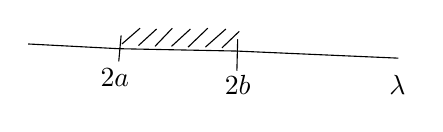
\begin{tikzpicture}[x=1cm,y=1cm]
\draw (-1.15,0.06)--(0,0)--(1.50,-0.03)--(3.55,-0.12);
\draw (0,-0.16)--(0.03,0.17);
\draw (1.50,-0.28)--(1.51,0.12);
\draw (0.04,0.06)--(0.27,0.26);
\draw (0.25,0.04)--(0.48,0.25);
\draw (0.46,0.03)--(0.68,0.26);
\draw (0.67,0.03)--(0.91,0.25);
\draw (0.88,0.02)--(1.13,0.26);
\draw (1.10,0.02)--(1.36,0.25);
\draw (1.31,0.01)--(1.53,0.22);
\node[below] at (-0.05,-0.13) {$2a$};
\node[below] at (1.51,-0.21) {$2b$};
\node[below] at (3.54,-0.21) {$\lambda$};
\end{tikzpicture}
\end{adjustbox}

$$
F(\lambda)\underset{\lambda\to\infty}{\longrightarrow}\frac2\lambda
$$

$\alpha,\beta,a,b$ нах. для компенсации полинома 2-й степени.

\underline{Ответ}
\begin{equation*}
F(g)=Z=-\frac12\sum_{k=1}^{\infty}
\frac{(72g^2)^k\Gamma\left(\frac{3k}{2}\right)}{\Gamma\left(\frac k2+1\right)(k+2)!}
\tag{12}
\end{equation*}

Крит. константа
\Unclear{GELFAND-P001301}{critical-value}{$g_c=\dfrac1{208\sqrt3}$},
особ. $F(g)\approx(g-g_c)^{5/2}$

\Incomplete{GELFAND-P001301}{right-edge-fragments}{На узкой полосе за правой границей листа видны три открывающие скобки «(» и обрезанные следующие штрихи; продолжения надписей находятся за краем кадра и не прочитаны.}

\SourcePage{GELFAND-P001302}{10}
Число триангуляций $F_n$ с $n$ верш. отсюда асимпт. находим
$$
F_n\sim n^{-7/2}g_c^{-2n}
$$
\underline{Возможное обобщение:} спиновые пер. в $\forall$ вершине триангуляции

\SourcePage{GELFAND-P001303}{unlabelled}
\underline{13.10.86 г.}\qquad \underline{Сем. Гельфанда}

\underline{\underline{Д. Гуревич.}}\qquad
\underline{Обобщенные алгебры и группы Ли.}

Постоянные реш. ур-й Янга-Бакстера
$$\Downarrow$$
обобщение теории Ли

аналогичное включению $(\text{супермат.})\supset(\text{матем.})$

\SourceFigure{GELFAND-P001303}{upper-right-marks}{Справа от записей о решениях уравнений и обобщении теории Ли — две почти вертикальные параллельные черты; правее вверху небольшой густо зачёркнутый знак.}

$$L,\quad \dim L=n$$
$$L^{\otimes2}\overset{S}{\longrightarrow}L^{\otimes2}
\qquad (\text{линейные отобр.})$$
$$L^{\otimes3}
\underset{\mathrm{id}\otimes S=S^{(2)}}{\overset{S\otimes\mathrm{id}=S^{(1)}}{\longrightarrow}}
L^{\otimes3}$$

(1) \underline{Ур-е Я.-Б.:}
$$1)\quad S^{(1)}S^{(2)}S^{(1)}=S^{(2)}S^{(1)}S^{(2)}$$
$$2)\quad S^2=\mathrm{id}\qquad
\overset{\mathrm{def}}{\Longleftrightarrow}\quad S\text{ — симметрия}$$

\underline{Обобщ. понятия алгебры Ли.}

$L$ — конечномерное вект. пр-во

Структ. обобщенной [окончание «ной» написано ниже строки] алгебры Ли (или $S$-алгебры) — это отображение

[Перед формулой зачёркнут знак:
\Unclear{GELFAND-P001303}{bracket-map-left-cancel}{неразборчиво}.]
$$L^{\otimes2}\overset{[\cdot,\cdot]}{\longrightarrow}L
\qquad\begin{gathered}(\text{линейное})\\\text{отображ.}\end{gathered}$$
[У конечного $L$ зачёркнут верхний показатель:
\Unclear{GELFAND-P001303}{bracket-map-superscript-cancel}{неразборчиво}.]

и вып. аксиомы
$$1)\quad [\cdot,\cdot]=-S[\cdot,\cdot]$$
($S$ — опер. симметрии, удовл. аксиомам $(1)_{1,2}$ и фиксир.)

(операторы пишутся справа)

$$2)\quad
\bigl(\mathrm{id}+S^{(1)}S^{(2)}+S^{(2)}S^{(1)}\bigr)
([\cdot,\cdot]\otimes\mathrm{id})[\cdot,\cdot]=0$$
[После первого знака $+$ зачёркнут знак перед $S^{(1)}$:
\Unclear{GELFAND-P001303}{axiom-two-cancel}{неразборчиво}.]

Здесь $\mathrm{id}=\mathrm{id}_{L^{\otimes3}}$

$$3)\quad S^{(1)}S^{(2)}([\cdot,\cdot]\otimes\mathrm{id})
=(\mathrm{id}\otimes[\cdot,\cdot])S$$

Лучше писать: $S^{(1)}=S^{(12)},\quad S^{(2)}=S^{(23)}$.

\SourceFigure{GELFAND-P001303}{lower-right-margin-stroke}{У самого правого края внизу видна часть тонкой изогнутой линии; оба конца дуги уходят за правую границу кадра.}

\SourcePage{GELFAND-P001304}{unlabelled}
$S$ — перестановка множителей $\Rightarrow$ что означают аксиомы?

Аксиомы (1) означают, что $S$ задает предс. группы подстановок
из 3-х элементов.

2) \underline{превр. в тождество Якоби} для $S$-перест., $[\ ,\ ]$ — коммут

3) тавтология в обычн. ситуации.

\underline{Супермат.}

\Unclear{GELFAND-P001304}{super-basis-initial-mark}{неразборчиво}
$t_1,\ldots,t_n$ — однор. базис
$$t_i\otimes t_j\overset{S}{\longrightarrow}
(-1)^{\operatorname{dt}t_i\cdot\operatorname{deg}t_j}\,t_j\otimes t_i$$
$$\operatorname{dt}[X,Y]=\operatorname{deg}X+\operatorname{deg}Y.$$
[Начертание оператора слева в двух местах:
\Unclear{GELFAND-P001304}{super-grading-notation}{dt}.]

\underline{Ещё пример:} цветные симметрии;
[Зачёркнуто: \Unclear{GELFAND-P001304}{colour-attribution-cancel}{неразборчиво}.]
\Unclear{GELFAND-P001304}{colour-attribution}{задан. у Мосолова}
(гр. Маслова)

\underline{Цветная математика}

$$S:\quad t_i\otimes t_j\longmapsto a(i,j)t_j\otimes t_i$$
(Посл. раб. \underline{Trostel}, 1984, J. Math. Phys., \underline{25}, $N=11$)

$a(i,j)$ должны \underline{удовл.} \underline{нек-рым} условиям
(выписывается из аксиом)

\Unclear{GELFAND-P001304}{drinfeld-first-word}{Косички}
в \Unclear{GELFAND-P001304}{drinfeld-abbreviation}{оконч.}
\underline{виде} \underline{придумал} Дринфельд.

Ассоциат. алгебры будут те же.

По асс. алгебре $S$-алгебра строится так:
$$[A,B]=AB-(AB)S$$
Точнее, есть опер. умн. $A^{\otimes2}\overset{\circ}{\longrightarrow}A$
$$[f,g]=(f\otimes g)\circ-((f\otimes g)S)\circ$$
Она будет удовл. всем аксиомам.

\underline{\underline{В. Казаков.}}\qquad
\underline{Ещё одна модель дискретн. 2-мерн. гравит.}

(Вася)

Рассм. триангул.
[Зачёркнут знак: \Unclear{GELFAND-P001304}{triangulation-cancel}{неразборчиво}.]
$S^2$, в вершинах расставим доп. перем. $\sigma_i=\pm1$
и возьмем статистику Изинга

$$(1)\quad Z_n=\sum_{\substack{\text{триан.}\\\text{сферы}}}
\sum_{\{\sigma_i\}}\exp[\beta G_{ij}\sigma_i\sigma_j]$$

\SourceFigure{GELFAND-P001304}{triangular-sketch}{Справа от формулы — треугольный контур с несколькими внутренними отрезками и повторно проведёнными наклонными линиями; буквенных подписей нет. Точное соединение линий в средней части не установлено.}

$G_{ij}$ — матр. смежности триангуляции,
$$G_{ij}=\begin{cases}
1,\ \text{если }i,j\text{ соседи}\\
0\quad\text{в прот. случае}
\end{cases}$$

\SourcePage{GELFAND-P001305}{14}
\Unclear{GELFAND-P001305}{top-cancellation}{[Перед первой строкой зачёркнута короткая группа букв; чтение не установлено.]}
Почему же модель КГ (квант. грав.)?
и какой КГ?

Рассм. непр. теорию
\begin{equation*}
Z=\int\mathcal{D}g\int\mathcal{D}\Psi\,
\exp\left(-\int d^2\xi\left[\mu\sqrt{g}
+\bar\Psi\sigma_\mu\partial_\mu\Psi
+g^{1/4}m\bar\Psi\Psi\right]\right)
\tag{2}
\end{equation*}
$\Psi$ — 2-мер. Майорановский фермион в кривом пр-ве/времени

$(2)\sim(1)$ \qquad Д-во сложное, \qquad $\sigma_\mu$ — матр. Паули

Реш. (2): \underline{Мигдал и Бершадский}

\begin{equation*}
\bar\Psi=i\Psi^T\sigma_2
\quad\text{— соотн. на майорановский фермион}
\end{equation*}
[Формула слева выделена нижней прямоугольной скобкой.]

($\Psi,\bar\Psi$ не независ., как у дираковских фермионов)

Вместо (1) далее описана более общ. (с магн. полем)
\begin{equation*}
Z_n=\sum_{\{G^{(n)}\}}\sum_{\{\sigma_i\}}
\exp\left[\beta\sum_{i,j=1}^{n}G_{ij}\sigma_i\sigma_j
+H\sum_i\sigma_i\right]
\tag{3}
\end{equation*}
[Справа, с охватывающей подпись скобкой:]
$G^{(n)}$ — граф с $n$ вершинами

Введем модель
\begin{equation*}
\begin{aligned}
Z(g)&=\sum_n g^n Z_n(\beta)
\overset{N\to\infty}{=}\frac{1}{N^2}\log
\int d^{N^2}u\int d^{N^2}v\,
\exp\bigl[-\operatorname{tr}(u^2+v^2-2cuv+\\
&\qquad\text{[зачёркнутый член]}\\
&\qquad+\frac{g(e^H u^3+e^{-H}v^3)}{\sqrt{N}}\bigr]
\end{aligned}
\tag{4}
\end{equation*}
\Incomplete{GELFAND-P001305}{matrix-cancelled-term}{[В зачёркнутом члене читаются $g e^H$, $u^3$, $N$, $e^{-H}$, $v^3$. Под левой группой видна дробная черта с $N$ ниже; слева от $v^3$ виден плюс. Остальные знаки и расположение множителей не удалось прочесть полностью.]}
\Unclear{GELFAND-P001305}{matrix-delimiters}{[После $\sqrt{N}$ видна закрывающая квадратная скобка; закрывающая круглая скобка для $\operatorname{tr}($ не читается. Оба видимых плюса, до зачёркнутой строки и в начале исправленной строки, сохранены.]}

[Под левым $Z(g)$ вписано $Z(g,c,H)$; между записями два коротких вертикальных штриха.]

$u,v$ — эрмитовы матрицы $N\times N$

Здесь $c=e^{-2\beta}$

Реш. в раб. Жюбера, Ициксона и $\ldots$

Конст. связи $g$ можно считать комплексной

\underline{И.М.Г.} Есть кн. \underline{Дайсона} (по русски): все разумные задачи в симм. пр-вах
при $N\to\infty$ имеют ответ.

\underline{Док-во ф-лы (4):} разложим $\exp$ $\Rightarrow$ диагр. техника;
верш. 2-х типов: $u$-верш. и $v$-вершины.

[Слева:]
\begin{center}
\begin{adjustbox}{max width=\linewidth}
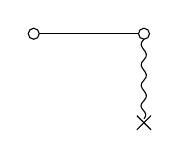
\begin{tikzpicture}[x=1cm,y=1cm]
\draw (0,0) circle (0.07);
\draw (1.4,0) circle (0.07);
\draw (0.07,0)--(1.33,0);
\draw (1.4,-0.07) .. controls (1.28,-0.18) and (1.51,-0.22) .. (1.4,-0.33)
 .. controls (1.28,-0.44) and (1.51,-0.48) .. (1.4,-0.59)
 .. controls (1.28,-0.70) and (1.51,-0.74) .. (1.4,-0.85)
 .. controls (1.28,-0.96) and (1.49,-0.98) .. (1.4,-1.08);
\draw (1.31,-1.04)--(1.49,-1.22);
\draw (1.31,-1.22)--(1.49,-1.04);
\end{tikzpicture}
\end{adjustbox}
\end{center}
[Справа:]
\begin{equation*}
\begin{adjustbox}{max width=\linewidth}
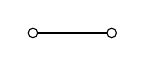
\begin{tikzpicture}[baseline=-0.1cm,x=1cm,y=1cm]
\draw (0,0) circle (0.06);
\draw (1,0) circle (0.06);
\draw (0.06,0)--(0.94,0);
\end{tikzpicture}
\end{adjustbox}
=\langle u^2\rangle=\frac{1}{1-c^2}=\langle v^2\rangle
\end{equation*}
[Под $\langle u^2\rangle$, с коротким вертикальным штрихом:]
ср. по гаус. распр.

\begin{equation*}
\begin{adjustbox}{max width=\linewidth}
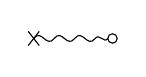
\begin{tikzpicture}[baseline=-0.1cm,x=1cm,y=1cm]
\draw (-0.07,-0.09)--(0.07,0.09);
\draw (-0.07,0.09)--(0.07,-0.09);
\draw (0,0) .. controls (0.10,0.13) and (0.16,-0.13) .. (0.26,0)
 .. controls (0.36,0.13) and (0.42,-0.13) .. (0.52,0)
 .. controls (0.62,0.13) and (0.68,-0.13) .. (0.78,0)
 .. controls (0.83,0.07) and (0.90,-0.07) .. (0.94,0);
\draw (1,0) circle (0.06);
\end{tikzpicture}
\end{adjustbox}
=\langle uv\rangle=\frac{c}{1-c^2}
\end{equation*}

\SourcePage{GELFAND-P001306}{unlabelled}
Что есть в модели (1)?

Фаз. переход (спонт. упорядочение спинов) при значении
\begin{equation*}
\beta_t^*=\frac12\ln(2\sqrt7+1).
\end{equation*}
[В слове «Фаз.» есть исправленные штрихи.]

\underline{Варченко}

\underline{Теор. Вика}
\begin{equation*}
\frac{1}{(2\pi)^{n/2}}\int e^{-\frac{x_1^2+\cdots+x_n^2}{2}}
\xi_1\cdots\xi_N\,dx
\overset{\mathrm{def}}{=}\langle\xi_1\cdots\xi_N\rangle
\end{equation*}
\Unclear{GELFAND-P001306}{gaussian-first-variable}{[Первый $x$ в показателе экспоненты исправлен поверх прежнего знака; видимая запись передана как $x_1^2$. Прежний знак не разобран.]}
Тогда
\begin{equation*}
\langle\xi_1\cdots\xi_N\rangle=
\sum_{\substack{\text{расст.}\\\text{скобок}}}
\langle\xi_{i_1}\xi_{i_2}\rangle\cdots
\langle\xi_{i_{N-1}}\xi_{i_N}\rangle
\end{equation*}
$\xi_j$ — лин. ф-и от $x_k$

\Unclear{GELFAND-P001306}{proof-cancelled-word}{[Перед «Д-во.» зачёркнуто слово; возможно «Решение».]}
\underline{Д-во.} сначала $\xi_i=x_{k_i}$ $\Rightarrow$ интеграл = произведению
и ост. воспольз. полилинейностью

\begin{equation*}
\int e^{-\operatorname{tr}u^2}u_{ij}u_{k\ell}\,du
=\delta_{i\ell}\delta_{jk}
\end{equation*}
\Unclear{GELFAND-P001306}{matrix-covariance-convention}{[Равенство переписано с видимой мерой $du$; нормирующий множитель здесь не записан.]}
\begin{equation*}
\int du\,e^{-\operatorname{tr}(u^2+\frac{g}{\sqrt N}u^3)}
=\sum\left(\frac{g}{\sqrt N}\right)^n
\int e^{-\operatorname{tr}u^2}(\operatorname{tr}u^3)^n\,du
\end{equation*}
\Unclear{GELFAND-P001306}{expansion-coefficient}{[У суммы не видно нижнего индекса; в написанном коэффициенте нет отдельного знака минус или факториала.]}

\begin{equation*}
\int e^{-\operatorname{tr}u^2}
\begin{adjustbox}{max width=\linewidth}
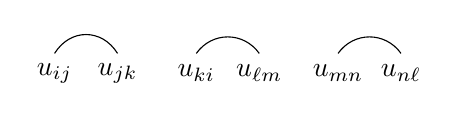
\begin{tikzpicture}[baseline=-0.1cm,x=1cm,y=1cm]
\node (a) at (0,0) {$u_{ij}$};
\node (b) at (0.8,0) {$u_{jk}$};
\node (c) at (1.8,0) {$u_{ki}$};
\node (d) at (2.6,0) {$u_{\ell m}$};
\node (e) at (3.6,0) {$u_{mn}$};
\node (f) at (4.4,0) {$u_{n\ell}$};
\draw (0,0.25) .. controls (0.2,0.57) and (0.6,0.57) .. (0.8,0.25);
\draw (1.8,0.25) .. controls (2,0.53) and (2.4,0.53) .. (2.6,0.25);
\draw (3.6,0.25) .. controls (3.8,0.53) and (4.2,0.53) .. (4.4,0.25);
\end{tikzpicture}
\end{adjustbox}
\,du
\end{equation*}
\Unclear{GELFAND-P001306}{paired-subscript-corrections}{[Под индексами $ki$ и $\ell m$ третьего и четвёртого множителей видны зачёркнутые индексы; их первоначальное чтение не установлено.]}

Расст. скобок $\Rightarrow$ [зачёркнуто: тройное произведение] граф.

\begin{center}
\begin{adjustbox}{max width=\linewidth}
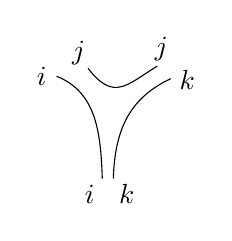
\begin{tikzpicture}[x=1cm,y=1cm]
\draw (0,1.4) .. controls (0.5,1.2) and (0.56,0.7) .. (0.58,0.1);
\draw (0.4,1.5) .. controls (0.73,1.07) and (0.90,1.3) .. (1.28,1.53);
\draw (1.45,1.37) .. controls (0.92,1.12) and (0.74,0.72) .. (0.72,0.1);
\node at (-0.19,1.4) {$i$};
\node at (0.28,1.7) {$j$};
\node at (1.33,1.75) {$j$};
\node at (1.66,1.36) {$k$};
\node at (0.42,-0.1) {$i$};
\node at (0.89,-0.1) {$k$};
\end{tikzpicture}
\end{adjustbox}
\qquad
$\delta_{ik}\delta_{kj}\delta_{km}\delta_{i\ell}\delta_{m\ell}\delta_{nn}$
\end{center}
\Unclear{GELFAND-P001306}{delta-second-factor}{[Второй множитель передан по видимым индексам: $\delta_{kj}$.]}

[Ниже слева:]
\begin{center}
\begin{adjustbox}{max width=\linewidth}
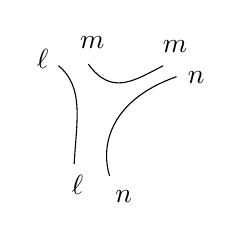
\begin{tikzpicture}[x=1cm,y=1cm]
\draw (0,1.4) .. controls (0.33,1.13) and (0.23,0.7) .. (0.2,0.15);
\draw (0.38,1.42) .. controls (0.67,1.02) and (0.95,1.2) .. (1.33,1.4);
\draw (1.5,1.26) .. controls (0.7,0.98) and (0.52,0.43) .. (0.65,0);
\node at (-0.2,1.49) {$\ell$};
\node at (0.43,1.69) {$m$};
\node at (1.48,1.64) {$m$};
\node at (1.75,1.25) {$n$};
\node at (0.24,-0.12) {$\ell$};
\node at (0.83,-0.26) {$n$};
\end{tikzpicture}
\end{adjustbox}
\end{center}
\SourceFigure{GELFAND-P001306}{lower-left-mark}{[В нижнем левом поле короткая тонкая волнистая черта, без подписи или видимой связи с диаграммами.]}
\SourcePage{GELFAND-P001307}{unlabelled}
\underline{20.10.86 г.}

\underline{\underline{Сем. Гельфанда.}}

\underline{В. Гинзбург.}

\underline{О раб. А. Гивенталя.}
\qquad (и потом о работе P. Deligne — L. Illusie)

\underline{Явный пример представления алгебры Гекке}

(возникающий из теории особенностей)

\begin{equation*}
\begin{aligned}
(1)\quad &\mathbb C^n\to\mathbb C^n\\
&(z_1,\ldots,z_n)\to\sigma_1(z),\ldots,\sigma_n(z)
\qquad\text{(элем. симм. многочлены)}
\end{aligned}
\end{equation*}

$n!$-листное накрытие над окрестн. общей точки.

Монодромия переставляет их.

(2)
\begin{equation*}
\begin{adjustbox}{max width=\linewidth}
\begin{tikzcd}[row sep=small, column sep=large]
\mathbb C^{n+1}\arrow[dd] & =\mathbb C^n\times\mathbb C\\
{} & \mathbb C\setminus\{z_1,\ldots,z_n\}\ \text{над }\sigma(z_1,\ldots,z_n)\arrow[d]\\
\mathbb C^n & \sigma(z)
\end{tikzcd}
\end{adjustbox}
\end{equation*}

В $\mathbb C^n\times\mathbb C$ удалим $\{z_1,\ldots,z_n\}$ над
\Unclear{GELFAND-P001307}{base-sigma-arguments}{$\sigma(z_1),\ldots,\sigma(z_n)$}.

\SourcePage{GELFAND-P001308}{20}
Из базы выкинем те $\sigma$, к-рые отвечают слившимся корням.

\begin{equation*}
\begin{adjustbox}{max width=\linewidth}
\begin{tikzcd}[row sep=large, column sep=small]
\mathbb C^{n+1}\arrow[d] & =\{(\sigma_1,\ldots,\sigma_n,z)\}\supset X=\{z^n+\sigma_1z^{n-1}+\ldots+\sigma_n=0\}\quad\text{(гиперпов.)}\\
\mathbb C^n\supset\Sigma & {}
\end{tikzcd}
\end{adjustbox}
\end{equation*}

$\Sigma$ — дискриминант (в $\mathbb C^n$).

\begin{equation*}
\begin{adjustbox}{max width=\linewidth}
\begin{tikzcd}[row sep=large]
\mathbb C^{n+1}\setminus X\arrow[d,"{\mathbb C\setminus\{z_1,\ldots,z_n\}}"]\\
\mathbb C^n\setminus\Sigma
\end{tikzcd}
\end{adjustbox}
\end{equation*}

Перейдем к 1-мерн. гомол. с коэффициентами

$f^\alpha$ — $\alpha$ — фикс. компл. число;
[Зачёркнуто: \Incomplete{GELFAND-P001308}{cancelled-function}{Два зачёркнутых слова не прочитаны.}]
многозн. ф-я

\begin{equation*}
f=z^n+\sigma_1z^{n-1}+\ldots+\sigma_n
\end{equation*}

$f^\alpha$ опред. накрытие; рассм. когомологии с коэфф. в нём

\Unclear{GELFAND-P001308}{cohomology-delimiter}{$H^1(\mathbb C\setminus\{\ast,\ast,\ldots,\ast\},f^\alpha\}$}

Есть предст. гр. кос $\Rightarrow$ фунд. группа (кос) $B(n)$,
зависит от пар. $\alpha$.

[Под $B(n)$: из $n$ нитей.]

фунд. группа $\mathbb C^n\setminus\Sigma=B(n)$.

\SourceFigure{GELFAND-P001308}{representation-links}{От правого края формулы $H^1$ загнутая стрелка направлена вниз к началу слов «фунд. группа (кос)». Внутри изгиба — небольшая подпись «(пр.)». Под словами «гр. кос» стоит повёрнутый вертикально знак равенства, ниже него — строка «фунд. группа $\mathbb C^n\setminus\Sigma=B(n)$». Точное присоединение верхней стрелки к строкам остаётся неуверенным.}

У гр. кос образующие $T_1,\ldots,T_{n-1}$ с соотн.
$T_1T_2T_1=T_2T_1T_2$.

($T_j$ отвеч. элем. обходу)

При этом предст. есть доп. соотнош.
$(T_i+1)(T_i-\alpha)=0\Rightarrow$

$\Rightarrow$ предст. пропуск. через предст. алг. Гекке

\SourceFigure{GELFAND-P001308}{braid-loops}{Слева нарисованы две чёрные точки на одной горизонтали. Их охватывает большой замкнутый вытянутый контур; на его верхней части стрелка направлена влево, на нижней — вправо. Внутри видны две пересекающиеся петли, похожие на восьмёрку вокруг этих точек; на верхнем диагональном участке стрелка направлена вправо, на нижнем — влево. Соединение линий в пересечениях не устанавливается уверенно.}

\begin{equation*}
\pi_1(\mathbb C^n\setminus\Sigma)=B(n)
\end{equation*}

образующие

\begin{center}
\begin{adjustbox}{max width=\linewidth}
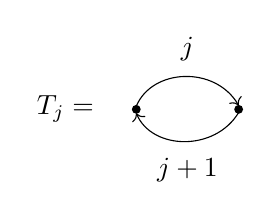
\begin{tikzpicture}
\node at (-1.55,0) {$T_j=$};
\fill (-0.65,0) circle (1.6pt);
\fill (0.65,0) circle (1.6pt);
\draw[->] (-0.65,0.04) .. controls (-0.45,0.52) and (0.35,0.56) .. (0.65,0.05);
\draw[->] (0.65,-0.04) .. controls (0.35,-0.54) and (-0.45,-0.52) .. (-0.65,-0.05);
\node at (0,0.77) {$j$};
\node at (0,-0.77) {$j+1$};
\end{tikzpicture}
\end{adjustbox}
\end{center}

(лин. преобр., отвечающее перестановке 2-х корней)

$\downarrow$

соединяем с $Id$.

\begin{equation*}
\begin{aligned}
1)\quad &T_iT_j=T_jT_i\quad\text{при }|i-j|\ge2\\
2)\quad &T_iT_{i+1}T_i=T_{i+1}T_iT_{i+1}\\
3)\quad &(T_i+1)(T_i-\alpha)=0
\end{aligned}
\end{equation*}

Цель была: доказать точность представл. фунд. группы в гр. матриц,
элементы к-рых — многочлены Лорана.

Для [зачёркнуто: \Unclear{GELFAND-P001308}{cancelled-n}{$n$}]
$n=3$ это известно.
[Справа слабая метка: \Unclear{GELFAND-P001308}{known-line-mark}{неразборчиво}.]

Спец. по теории группы Кос называют это представлением
\Unclear{GELFAND-P001308}{burau-name}{Бурао}.

$\alpha=-1\Rightarrow$ гр. монодромии эллипт. интегралов
(гиперэлл. кривой)

[Вписано над скобкой, с изогнутым соединительным штрихом:
\underline{монодр.}]

\SourcePage{GELFAND-P001309}{unlabelled}
\underline{Бейлинсон}

\underline{о раб. P. Deligne и L. Illusie.}\qquad Preprint Orsay

Алгебраические док-ва фактов, к-рые раньше док. только трансценд. методами

(опер. Лапласа и т.п.)

$X$ — гладкое компактное алг.
\Unclear{GELFAND-P001309}{variety-abbreviation}{м-ие} над $\mathbb C$

\underline{Комп. де Рама:}

\Unclear{GELFAND-P001309}{de-rham-coefficient}{$H^\bullet_{DR}(X)=H^\bullet(X,O\to\Omega^1\to\Omega^2\to\ldots)$}

[Под левой частью формулы:] в топ. Зарисского

[Под $\Omega^1$, $\Omega^2$, с соединительными штрихами:]
алгебр. дифф. формы

\underline{\underline{Теор.}}
\begin{equation*}
E_1^{p,q}=H^p(X,\Omega^q)
\end{equation*}

(спектр. посл. вырождается уже в 1-м члене)

1-е [Вписано над строкой, с указателем вставки: алг.] док-во —
Фалтингс — неэлем.

\underline{Deligne} и \underline{Illusie} — элементарн. алгебраич.

\underline{Идея док-ва:} вместо $\Delta$ использ. редукция в хар-ку $p$!!

$X/k$ над конечн. полем $k$ или
[Зачёркнуто: \Incomplete{GELFAND-P001309}{cancelled-field}{Зачёркнутое слово перед «полем» не прочитано.}]
[Вписано сверху, с указателем вставки: \underline{совершенным}]
полем конечн. хар-ки

Есть когомологии.

\underline{Казаков В.} (продолжение).

\underline{Ф-ла, на к-рой основано вычисление $2^{\text{х}}$-матричного интеграла}

\begin{equation*}
(1)\quad
\int d(\Omega)_{U(N)}e^{\operatorname{tr}(\lambda\Omega^+\mu\Omega)}
=\left(\prod_{k=1}^{N-1}k!\right)
\frac{\det_{i,j}e^{\lambda_i\mu_j}}{\Delta(\lambda)\Delta(\mu)}
\end{equation*}

$\lambda,\mu$ — диагональные матрицы

\begin{equation*}
\Delta(\lambda)=\prod_{i>j}(\lambda_i-\lambda_j)
\end{equation*}

\begin{equation*}
\lambda=\begin{pmatrix}
\lambda_1 & & \\
&\ddots&\\
&&\lambda_N
\end{pmatrix},\qquad
\mu=\begin{pmatrix}
\mu_1&&0\\
&\ddots&\\
0&&\mu_N
\end{pmatrix}
\end{equation*}

Впервые в раб. Ициксона, Зюбера. Док: с пом. ур. теплопров. на гр. матриц.

\underline{И.М.Г.} Похожая ф-ла есть в кн. \underline{Гельфанд},
\underline{Наймарк} «Унит. предст. класс. групп» (1951)

\begin{equation*}
\Omega^{-1}\lambda\Omega=H
\qquad
\Delta_1^{\mu_1}\Delta_2^{\mu_2}\ldots\Delta_n^{\mu_n}
\end{equation*}

$\Omega$ — унит.

$\lambda$ — диаг. ($\lambda_i>0$)

(основн. миноры)

\begin{center}
\begin{adjustbox}{max width=\linewidth}
\begin{tikzpicture}
\draw (0,0) rectangle (3,-2.7);
\draw (0.55,0) -- (0.55,-0.55) -- (0,-0.55);
\draw (1.1,0) -- (1.1,-1.1) -- (0,-1.1);
\node at (0.28,-0.28) {$\Delta_1$};
\node at (0.82,-0.82) {$\Delta_2$};
\end{tikzpicture}
\end{adjustbox}
\end{center}

\SourcePage{GELFAND-P001310}{21}

\begin{equation*}
\int \Delta_1^{\mu_1}\Delta_2^{\mu_2}\ldots\Delta_n^{\mu_n}\,d\Omega
=\left|\begin{array}{cccc}
\lambda_1^{\mu_1}&\lambda_1^{\mu_2}&\ldots&\lambda_n^{\mu_n}\\
\lambda_2^{\mu_1}&\lambda_2^{\mu_2}&\ldots&\lambda_n^{\mu_n}\\
-&-&-&-
\end{array}\right|
\left[\prod(\lambda_i-\lambda_k)\prod(\mu_i-\mu_k)\right]^{-1}
\tag{2}
\end{equation*}
\Unclear{GELFAND-P001310}{top-determinant}{Последний элемент обеих выписанных строк: $\lambda_n^{\mu_n}$? Нижняя строка состоит из коротких горизонтальных штрихов.}
\Unclear{GELFAND-P001310}{top-differential}{В $d\Omega$ нижняя левая часть $\Omega$ переписана; первоначальный знак не различается.}

(написан в статье Г. и Н.)

Отсюда получ. теор. \underline{Лидского} о соб. знач. произвед. матриц (эрмитовых)
[Под словом «эрмитовых»: $H_j>0$.]

Какие они могут быть?

Соб. знач. у $H_1H_2$ всегда $>0$. Область описывается.

\underline{Док.} с пом. эллипт. координат (обобщенных)

К. \underline{Док-во ф-мы (1).}

Напишем ур. теплопров. на эрм. матрицах
\begin{equation*}
\left(\frac{\partial}{\partial t}-\frac12\Delta_u\right)f(t,u,v)=0,
\quad t>0;\qquad \left.f\right|_{t=0}=\delta(u-v)
\tag{3}
\end{equation*}
\begin{equation*}
f(t,u,v)=\frac{1}{(2\pi t)^{N^2/2}}
e^{-\frac{1}{2t}\operatorname{tr}(u-v)^2}
\tag{4}
\end{equation*}
\Unclear{GELFAND-P001310}{heat-exponent}{Показатель у $(2\pi t)$: $N^2/2$? / $N/2$?}

$\Delta_u=\sum$ 2-х произв. по $\operatorname{Re}$ и $\operatorname{Im}$ элементов (вкл. диагон.)

\begin{equation*}
g(t,u)=\int d^{N^2}v\,f(t,u,v)g(0,v)
\tag{5}
\end{equation*}

Перех. к пер. Дайсона (перем. в терминах соб. значений), счит. что $g$
[над $g$ вписано $(0,v)$, к нему проведена изогнутая линия]
зав. только от соб. знач. $v$

\begin{equation*}
g(t,\mu)=\int d(\Omega)\int\prod d\lambda\,\Delta^2(\lambda)
f(t,\mu,\Omega^+\lambda\Omega)g(0,\lambda)
\tag{6}
\end{equation*}
[На правом поле, после двойного вертикального штриха: тогда $g(t,u)$ тоже.]

\begin{equation*}
u=\Omega_1^+\mu\Omega_1,\qquad v=\Omega_2^+\lambda\Omega_2;
\quad\text{тогда}\quad\Omega=\Omega_2\Omega_1^+
\end{equation*}
\begin{equation*}
\underbrace{\Delta(\mu)g(t,\mu)}_{\xi(t,\mu)}
=\int\prod d\lambda\,K(t;\mu,\lambda)\Delta(\lambda)g(0,\lambda)
\tag{7}
\end{equation*}

Здесь
\begin{equation*}
K(t,\mu,\lambda)=\Delta(\lambda)\Delta(\mu)
\int d(\Omega)\,f(t,\mu,\Omega^+\lambda\Omega)
\tag{8}
\end{equation*}
[В конце строки зачеркнуто:
\Unclear{GELFAND-P001310}{kernel-cancelled}{$e^{-\operatorname{tr}(\lambda-\Omega^+\mu\Omega)}$?}.]

[Ниже отдельно написано:
\Unclear{GELFAND-P001310}{kernel-separate}{$e^{-\operatorname{tr}(\lambda-\Omega^+\mu\Omega)^2}$}.]

Для $\xi(t,\mu)$ [зачеркнуто:
\Unclear{GELFAND-P001310}{xi-cancelled-word}{напишем? / написано?};
над строкой вписано «выполняется», к месту вставки проведена изогнутая линия]
ур-е (!)
\begin{equation*}
\left(\frac{\partial}{\partial t}-\frac12\sum_{i=1}^{N}
\frac{\partial^2}{\partial\lambda_i^2}\right)\xi(t,\lambda)=0,
\quad t>0.
\tag{9}
\end{equation*}
[Перед $\xi$ зачеркнут знак:
\Unclear{GELFAND-P001310}{xi-cancelled-function}{$f$? / $g$?}.]

Хотя
\begin{equation*}
\left(\frac{\partial}{\partial t}-\frac12\Delta_\lambda\right)g(t,\lambda)=0,
\quad\text{где}\quad
\Delta_\lambda=\frac{1}{\Delta(\lambda)^2}
\sum_i\frac{\partial}{\partial\lambda_i}
\left(\Delta^2(\lambda)\frac{\partial}{\partial\lambda_i}\right)
\tag{10}
\end{equation*}

\underline{И.М.Г.}: это есть в кандидатской дисс. Ф.А. Березина: Труды ММО ($\approx1956$г.)

\SourcePage{GELFAND-P001311}{unlabelled}

Подставляя $\dfrac{\xi(t,\lambda)}{\Delta(\lambda)}=g(t,\lambda)$ в (10), приходим к (9).

\underline{И.М.Г.} Сделал Березин, многократно использовал Хариш-Чандра.

\underline{К.} Пишем теперь $\xi(t,\lambda)$ и т.п.

\underline{Вопрос}: как считать интеграл
\begin{equation*}
\int d\Omega\,e^{\operatorname{tr}(\lambda_1\Omega\mu_1\Omega^+)+\operatorname{tr}(\lambda_2\Omega\mu_2\Omega^+)}
\tag{11}
\end{equation*}

— решение кирального поля на $U(\infty)$

в принципе сосчитан (Вигман и Поляков решили кир. поле —
\newline
— редукция Егучи—Каваи)

Самое интересное связано с хромодинамикой
\begin{equation*}
\int\prod_{\mu=1}^{d}d\Omega_\mu\,
\exp{\sum_{\mu\ne\nu}\operatorname{tr}(\Omega_\mu^+\Omega_\nu^+\Omega_\mu\Omega_\nu)}
\tag{12}
\end{equation*}

\underline{не сосчитан и калибр. теория не решена}

Здесь сидит вся $d$-мерн. физика (достат. $d\le4$)

(12) — Статсумма Я.-М. на решетке.

\SourcePage{GELFAND-P001312}{unlabelled}

\underline{\underline{27/X-86г.}}\qquad \underline{Сем. Гельфанда.}

\underline{Захаревич}

$V$ — пр-во эрмитовых матриц $N\times N$

Рассмотрим ф-ю $g(t,x)$, $t\in\mathbb R$, $x\in V$

и ур-е теплопроводности
\begin{equation*}
g_t=\Delta g
\tag{1}
\end{equation*}

\underline{Утв.}
\begin{equation*}
\int_{U(N)}d\Omega\,e^{\operatorname{tr}(\lambda\Omega^+\mu\Omega)}
=\left(\prod_{k=1}^{N-1}k!\right)
\frac{\det\Vert e^{\lambda_i\mu_j}\Vert}{\Delta(\lambda)\Delta(\mu)},
\tag{2}
\end{equation*}
\begin{equation*}
\lambda=\operatorname{diag}(\lambda_i),\qquad
\mu=\operatorname{diag}(\mu_i);
\end{equation*}
\begin{equation*}
\Delta(\lambda)=\prod_{i>j}(\lambda_i-\lambda_j)
\end{equation*}

И.М.Г. Такие интегралы еще считали И.М.Гельфанд, Наймарк, Гиндикин и Карпелевич, Фатеев,

Важно: это \Unclear{GELFAND-P001312}{combinatorial-verb}{связывается? / связывался?}
с комбинаторной зад. о триангуляциях сферы.

\underline{Зад.}, из к-рой возникла теор. предст.:
\begin{equation*}
H_1H_2\qquad H_j^*=H_j>0.
\end{equation*}
Известны соб. знач. $H_j$; как распредел. соб. знач. $H_1H_2$?

Эллиптич. коорд. на мн-ве унит. матриц

\SourceFigure{GELFAND-P001312}{ellipsoid-section}{Слева нарисован горизонтально вытянутый овал. Через него проходит узкий наклонный четырехугольник, выступающий сверху и снизу; внутри овала виден вытянутый наклонный контур с прерывистой левой частью. Подписей и стрелок нет. Точные сопряжения сплошных и прерывистых линий требуют проверки по скану.}

Рассм. эллипсоид с осями $a,b,c$

$a_1,b_1$ — оси эллипса, получ. в сечении
\begin{equation*}
a\le a_1\le b\le b_1\le c
\end{equation*}

\begin{equation*}
\begin{array}{ccccccc}
a&&b&&c&&d\\
&a_1&&b_1&&c_1&\\
&&a_2&&b_2&&\\
&&&a_3&&&
\end{array}
\end{equation*}

Надо вычислить $d\Omega$ для матриц 2-го порядка.
\begin{equation*}
\int a_{11}^{\lambda_1}
\left|\begin{array}{cc}a_{11}&a_{12}\\a_{21}&a_{22}\end{array}\right|^{\lambda_2}
\ldots\ d\Omega,
\end{equation*}
$\lambda_j$ — произв. параметры;

$\mu$ — фиксир. диаг. матрица.
\begin{equation*}
A=\Omega^+\mu\Omega
\end{equation*}
$\mu$ дано

\underline{Спектр. анализ}: анализ в $\mathbb R^N$ (или $\mathbb C^N$) при $N\to\infty$.

\underline{Вопрос для школьников}: какую часть 1000-мерного арбуза составляет слой толщины $\dfrac{R}{100}$
окруж. экватор. плоскость. \underline{Ответ}: почти всё.

\SourcePage{GELFAND-P001313}{24}

\underline{Дан симплекс} (\Unclear{GELFAND-P001313}{simplex-dimension}{1000-мерный}): частица отраж. от граней;
[зачёркнуто: \Incomplete{GELFAND-P001313}{top-cancelled}{Зачёркнутое короткое слово не прочитано; возможное «она» не установлено.}]
какую часть времени она проведёт в
$\Unclear{GELFAND-P001313}{neighborhood-fraction}{\frac{1}{100}}$-окр. граней?
\underline{ответ}: почти всё время.

\underline{\Unclear{GELFAND-P001313}{lidskii-initial}{Б.} Лидский.}
\underline{Отобр. моментов;}
рассм. эрмит. матр. с фиксир. соб. значениями и на них отображение
\begin{equation*}
H\longrightarrow\text{диагональ }H
\end{equation*}
Написано \Unclear{GELFAND-P001313}{fourier-abbreviation}{преобр.} Фурье отобр. моментов.

\underline{И.М.Г.} Что такое \Unclear{GELFAND-P001313}{super-analogue}{супераналог} симметрической группы?

\underline{В. Гинзбург:} Идея: найти критич. точки отображения.
Взять 1-й член асимптотики — он будет точной ф-лой по теор.
\Unclear{GELFAND-P001313}{dh-name}{Дюйстерм.}-Хекмана.

\underline{Примерная формулир. теор. Д.-Х.}
$(M,\omega)$ — замкн. симпл. мн-ие.
\begin{equation*}
\int_M e^{iH(x)}\omega^n(x)
=(2\pi)^{-n}\sum_{\Unclear{GELFAND-P001313}{dh-critical-condition}{H''(x_k)=0}}
\frac{e^{iH(x_k)}}{\sqrt{\det\frac{\partial^2H}{\partial x_i\partial x_j}}}
\end{equation*}
\begin{equation*}
dH(\cdot)=\omega(\xi,\cdot)
\end{equation*}

\underline{Условие}: \Unclear{GELFAND-P001313}{periodic-flow}{фаз.} поток $\xi$ должен быть периодичен.

\underline{Семенов-Тян-Шанский} показал, что это совп. с
[вставлено над строкой: ф-лой] Кириллова в случае орбиты.

Идея: $i\Omega^+\mu\Omega$ — орбита, на к-рой есть симп. структура
\begin{equation*}
M=\text{фактор унит. матриц по диагональной}
\end{equation*}
\begin{equation*}
X=\Omega^+\mu\Omega;
\end{equation*}
\begin{equation*}
\omega(X)(\xi,\eta)=\operatorname{tr}(X\cdot[\xi,\eta]),
\qquad \xi,\eta\in T_X
\end{equation*}

\tikz[baseline=(g1313.base)]{\node[draw,circle,inner sep=1pt] (g1313) {!};}
\underline{Вопрос И.М.Г.:} когда нужен и 2-й член асимптотики?
Проанализировать топологич. причины, по к-рым 2-й член 0 и т.д.
Связь с нер-вами Морса.

Для каких интегралов 1-й член асимпт. даёт точный ответ?

\underline{Способ}: смотрим, когда 2-й член асимптотики $=0$ на соврем. уровне.

\underline{Подзадача}: для того, чтобы возникли характерист. числа.

\underline{Гипотеза (моя)}: вместо
[зачёркнуто: \Unclear{GELFAND-P001313}{hypothesis-cancellation}{неразборчиво}]
$S^1$-действия задать действие нильпотентной гр. Ли
(напр., 2-мерной $\Rightarrow$ возникнут 2 члена)

[У левого обрезанного края, внизу:]
\Unclear{GELFAND-P001313}{margin-left-fragment}{фрагмент дроби: верхний знак неразборчив; видны дробная черта и окончание знаменателя «00»}

\SourcePage{GELFAND-P001314}{unlabelled}

\underline{3/$\overline{\underline{\mathrm{XI}}}$-86 г.}\qquad \underline{Сем. Гельфанда.}

\underline{Г. Ольшанский.}

\begin{equation*}
\begin{aligned}
\text{(1)}\quad &\int_{U(n)}
\Delta_1(uRu^{-1})^{\sigma_1-\sigma_2}\cdots
\Delta_{n-1}(uRu^{-1})^{\sigma_{n-1}-\sigma_n}
\Delta_n(uRu^{-1})^{\sigma_n}\,du
\\
&=c_n\det\bigl[r_i^{\Unclear{GELFAND-P001314}{determinant-exponent}{\sigma_j+n-j}}\bigr]
\left(\prod_{i<j}(r_i-r_j)\prod_{i<j}(\sigma_i-\sigma_j+j-i)\right)^{-1};
\end{aligned}
\end{equation*}
[В показателе при элементе определителя — наложенные и зачёркнутые штрихи.]

\begin{equation*}
\Unclear{GELFAND-P001314}{diagonal-letters}{R=\operatorname{diag}(r_1,\ldots,r_n),\quad r_i>0}
\end{equation*}
$\Delta_m$ — гл. миноры матриц в скобках
\begin{equation*}
c_n=1!2!\ldots(n-1)!
\end{equation*}

\SourceFigure{GELFAND-P001314}{callout-line}{Угловая выносная линия под началом правой части формулы: идёт вправо под знаком равенства и началом определителя, затем вниз, вправо и вниз вдоль правой границы пояснения о $\Delta_m$. Наконечников стрелок не видно.}

— интеграл \Unclear{GELFAND-P001314}{book-preposition}{из} книги Гельфанда-Наймарка

Из (1) выводится ф-ла (2) на стр. 24.

[У левого обрезанного края:]
\Unclear{GELFAND-P001314}{left-edge-fragment}{обрезанное окончание «ми» или «ши»; ниже отдельные обрезанные штрихи}
[Ниже видна стрелка $\nearrow$; под ней — обрезанный крючкообразный штрих и отдельный нижний след, возможно край вопросительного знака.]

\SourcePage{GELFAND-P001315}{unlabelled}

\underline{Д-во (1).}\qquad (1) $=$ ф-ла характеров Г. Вейля.

$e_1,\ldots,e_n$ — кан. базис
\begin{equation*}
u e_i=f_i
\end{equation*}

\underline{Рассм.} $GL_n$ и её унит. предст. класса I
(т.е. $\exists$ вектор, инвар. отн. компактной подгруппы);
пусть $\xi_0$ — вектор, $T_u\xi_0=\xi_0$

Рассм. [зачёркнуто: вектор; над строкой: ф-ю] $(T_g\xi_0,\xi_0)$

Если предст. реализ. на пр-ве флагов, то эта ф-я пишется в виде
интегр. вида (1) и он — сферич. ф-я $GL_n$ отн. унит. подгруппы,
и т.д.

\underline{И.М.Г.} Общий вопрос: какие интегралы таким образом считаются?

\begin{adjustbox}{max width=\linewidth}
\begin{tikzpicture}[baseline=(speaker1315.base)]
\node[anchor=base west,inner sep=0pt] (speaker1315) at (0,0) {Дринфельд В.};
\draw[->] (0,-0.08) -- (2.75,-0.08);
\draw (0,-0.15) -- (3.15,-0.15);
\end{tikzpicture}
\end{adjustbox}
\qquad \underline{Квантование KdV по Белавину}

Об одной идее Белавина.

Квантование KdV раньше делалось неправильно.

KdV гамильт. относит. $2^{\text{х}}$ скобок Гельфанда-Дикого

Какая нужна? Надо квант. отн. обеих скобок.

Любая их лин. комб. — тоже скобка.

Надо ввести 2 постоянные Планка!

\begin{equation*}
\text{(1)}\quad u_t=u_{xxx}+uu_x
\end{equation*}

Скобки:
\begin{equation*}
\text{(2)}\quad \mathrm{II}:\ -\frac12\partial^3-u\partial-\partial u;
\qquad \mathrm{I}:\ -2\partial
\end{equation*}
— гамильт. операторы этих скобок

Это значит, что
\begin{equation*}
\text{(3)}\quad
\{u(x),u(y)\}=\lambda_1
\Unclear{GELFAND-P001315}{source-brackets}{[-\frac12\partial^3-u\partial-\partial u)\delta(x-y)]}
-2\lambda_2\partial\delta(x-y),
\end{equation*}
где $\partial=\frac{\partial}{\partial x}$

Идея гамильт. оператора восх. к Березину (предложил матрицу, обратную к симплектической)

После квантования (3) получаем.
\begin{equation*}
\text{(4)}\quad
[u(x),u(y)]=h_1\left(-\Unclear{GELFAND-P001315}{quantum-coefficient}{\frac12}\partial^3-u\partial-\partial u\right)\delta(x-y)
-2h_2\partial\delta(x-y),
\end{equation*}

\underline{И.М.Г.} Нет ни одного нелинейного ур-я, к-ое
\Unclear{GELFAND-P001315}{gelfand-adverb}{как} следует проквантовано.

Первые опыты — квантовые группы.

Предложение: делать \Unclear{GELFAND-P001315}{measure-through}{чрз}
\Unclear{GELFAND-P001315}{measure-perturbation}{возмущение} меры.
$P(\varphi)_2$ делается так,

\underline{Др.} Никто не сравнивал квант. по Фаддееву и по
Albeverio-\Unclear{GELFAND-P001315}{last-name}{Høegh-Kron'у}

\SourcePage{GELFAND-P001316}{28}

\underline{Др.} Будем заниматься только 2-й скобкой.

\begin{equation*}
[u(x),u(y)]=h\left(-\frac{1}{2}\partial^3-u\partial-\partial u\right)\delta(x-y)
\tag{5}
\end{equation*}

Получается алгебра Вирасоро
\qquad ($h$ — параметр центрального расширения)

Пуасс. \Unclear{GELFAND-P001316}{poisson-abbreviation}{м-ие / м-же}
— орбита коприсоед. предст. алг. Вирасоро;
квант. — по Кириллову.

$\exists$ счётное число ф-лов-интегралов в инволюции
\begin{equation*}
F_n(u)=\int\varphi_n(u,u',\ldots,u^{(n)})\,dx
\tag{6}
\end{equation*}

Квант. аналог?

$u$ и $u'$ не коммутируют.

Замолодчиков: есть квант. аналог
[зачёркнуто: \Unclear{GELFAND-P001316}{quantum-cancel}{знак, похожий на $\varphi$ или $\varphi_n$}]
$F_n$

не будем думать о гамильт.

Преобр. Миуры
\begin{equation*}
u=v'-v^2
\tag{7}
\end{equation*}

Оно \Unclear{GELFAND-P001316}{miura-adjective}{пуассаново / пуассоново}, если на $\{u\}$ — 2-я ск. Г.-Д

\begin{equation*}
\text{на }\{v\}\quad-\quad\{v(x),v(y)\}=\delta'(x-y)
\end{equation*}

\begin{equation*}
[v(x),v(y)]=h\delta'(x-y)\qquad(x\in S^1)
\tag{8}
\end{equation*}

— алг. Гейзенберга;
\Unclear{GELFAND-P001316}{fourier-insertion}{[перед «разложить» зачёркнут знак, похожий на «И»; над строкой вставлено «надо», к началу слова проведена линия]}
разложить в ряд Фурье
[зачёркнуто: \Unclear{GELFAND-P001316}{fourier-cancel}{$v$ / $\xi$}]
и получим:

\begin{equation*}
[v_m,v_n]=hm\delta_{m,-n}I
\tag{9}
\end{equation*}

[Справа от (9):] (1-мерн. расшир. коммут. алгебры)

2 беск.-мерные алг. Ли (обёрт. алг.):

а) \underline{алг. Гейзенберга}\qquad б) \underline{алг. Вирасоро}

\underline{Утв.} Имеется простой гомом. из обёрт. алг. б) в обёрт. алг. а)

Генер. Вирасоро $\to$ квадр. выраж. от Гейзенберга.

Алг. Вирасоро:
\begin{equation*}
L_n=e^{in\varphi}\frac{d}{d\varphi}\qquad(\text{на }S^1)
\tag{10}
\end{equation*}

и 1-мерн. расширение с пом. цикла Гельфанда — Фукса.

Фукс: соотв. преобр. из (9) в (10)

\begin{equation*}
\begin{aligned}
v_i,\ i\ne0,\qquad &L_n=(\alpha n+\beta)v_n+\sum_{\substack{p+q=n\\p>q}}v_pv_q\\
\text{\underline{алг. Гейзенберга}}\qquad &n\ne0
\end{aligned}
\tag{11}
\end{equation*}

Это и есть преобр. Миуры.

[Зачёркнута формула:
\Unclear{GELFAND-P001316}{cancelled-commutator}{$[v_n,v_m]=h$ / $[v_m,v_n]=h$}.]

\begin{equation*}
[L_n,L_m]=(m-n)L_{n+m}+\delta_{n,-m}\frac{n^3-n}{12}c,
\qquad c\text{ коммут. со всеми }L_n
\end{equation*}
\Unclear{GELFAND-P001316}{commutator-factor}{[Коэффициент $(m-n)$ передан как в рукописи.]}

Квантование $=$ вложение в обёрт. алг. алгебры [окончание «ры» вписано ниже строки] Гейзенберга.

Задача (интересная): написать все гамильтонианы
\SourcePage{GELFAND-P001317}{unlabelled}
$KdV$ связано с опер. \Unclear{GELFAND-P001317}{top-sturm-liouville}{Шт.-Лиувилля}:
\begin{equation*}
L=\partial^2+u.\tag{12}
\end{equation*}
\Incomplete{GELFAND-P001317}{crossed-line-before-generalization}{Зачёркнутая строка перед словами «как обобщить» не поддаётся надёжному чтению.}

как обобщить на высший порядок
\begin{equation*}
L=\partial^n+u_{n-2}\partial^{n-2}+\ldots+u_0\tag{13}
\end{equation*}
и есть аналог пр. Миуры (Wilson, Дринфельд, Соколов).

Опер. (13) связан с $sl(n)$.

Вместо
\begin{equation*}
u=v'-v^2
\end{equation*}
правильней писать;

\Unclear{GELFAND-P001317}{margin-left-loop}{неразборчивый петлеобразный знак на левом поле}
\begin{equation*}
L=\partial^2+u=(\partial-v)(\partial+v)\tag{14}
\end{equation*}
Разложим:
\begin{equation*}
\begin{gathered}
L=\partial^n+u_{n-2}\partial^{n-2}+\ldots+u_0
=(\partial+v_1)\ldots(\partial+v_n),\\
v_1+\ldots+v_n=0
\end{gathered}\tag{15}
\end{equation*}
Получается преобр. Миуры.

Это связано с Пикаром-Вессио.
\begin{equation*}
\{u(x),u(y)\}=
\left(-\frac12\partial^3-u\partial-\partial u\right)\delta(x-y)\tag{16}
\end{equation*}
\begin{center}
\begin{adjustbox}{max width=\linewidth}
\begin{tikzpicture}[x=1cm,y=1cm]
\draw[->] (0,1.2) .. controls (-0.3,1.1) and (0.2,0.9) .. (0,0.8)
.. controls (-0.2,0.65) and (0.2,0.5) .. (0,0.35)
.. controls (-0.15,0.2) and (0.15,0.15) .. (0,0);
\node[right] at (0.35,0.7) {коэфф. Фурье};
\end{tikzpicture}
\end{adjustbox}
\end{center}
\begin{equation*}
\{u_i,u_j\}=\text{квадр. соотн.}\tag{17}
\end{equation*}
\textit{[В формуле (17), непосредственно после $u_i$, перед запятой:}
\Incomplete{GELFAND-P001317}{equation-17-first-cancelled-group}{Плотно заштрихованная группа знаков неразборчива.}
\textit{]}

\textit{[В формуле (17), непосредственно после $u_j$, перед правой фигурной скобкой:}
\Incomplete{GELFAND-P001317}{equation-17-second-cancelled-group}{Плотно заштрихованная группа знаков неразборчива.}
\textit{]}

\Incomplete{GELFAND-P001317}{cancelled-word-above-fateev}{Зачёркнутое слово над фамилией Фатеев не поддаётся чтению.}

Фатеев, Замолодчиков получили $\overset{(n=3)}{\text{ф-лы}}$, решающие задачу.

\underline{Б. Фейгин} что-то сделал (1986 г., апрель): обобщ. на $sl(3)$
\begin{center}
конф. на ВДНХ
\end{center}

\underline{Склянин}: квант. $KdV$ на конечном отрезке с краев. условиями.

\Incomplete{GELFAND-P001317}{cancelled-initials-above-img}{Зачёркнутая короткая запись над «И.М.Г.» не поддаётся надёжному чтению.}

\underline{И.М.Г.} Метод прогонки (Гельф., Локуциевский) аналогичен преобр. Миуры.
\begin{equation*}
y''-a(x)y=0
\end{equation*}
\begin{center}
\begin{adjustbox}{max width=\linewidth}
\begin{tikzpicture}[x=1cm,y=1cm]
\draw (0,0)--(2,0);
\draw (0,-0.13)--(0,0.13);
\draw (2,-0.13)--(2,0.13);
\node[below] at (0,-0.08) {$0$};
\node[below] at (2,-0.08) {$0$};
\node[right] at (3.1,0) {$0$ на концах};
\end{tikzpicture}
\end{adjustbox}
\end{center}
Нельзя $\exp$ растущее решение брать (точность теряется).

($\Rightarrow$ нельзя 2 лин. незав. решения)

\SourcePage{GELFAND-P001318}{29}
\begin{center}
\begin{adjustbox}{max width=\linewidth}
\begin{tikzpicture}[x=1cm,y=1cm]
\draw (0,0)--(3.4,0);
\draw (0,-0.17)--(0,0.17);
\draw (0.67,-0.12)--(0.67,0.12);
\draw (1.18,-0.15)--(1.18,0.15);
\draw (1.67,-0.13)--(1.67,0.13);
\draw (2.05,-0.12)--(2.05,0.12);
\draw (2.39,-0.11)--(2.39,0.11);
\draw (2.72,-0.1)--(2.72,0.1);
\draw (3.06,-0.1)--(3.06,0.1);
\draw (3.4,-0.18)--(3.4,0.18);
\node[below] at (0,-0.1) {$0$};
\end{tikzpicture}
\end{adjustbox}
\end{center}
Переносим краев. условие в соседнюю точку
\begin{equation*}
y'(0)+\alpha y(0)=0.
\end{equation*}
В соседней точке $\alpha$ меняется:
\begin{equation*}
\alpha'-\alpha^2=0\quad (!)\quad\text{— Миура.}
\end{equation*}
\Unclear{GELFAND-P001318}{miura-source-comparison}{В источнике $\alpha'-\alpha^2=0$ (!); сопоставление с $y''-a(x)y=0$ предыдущего кадра остаётся неразрешённым.}
Для $n$-го порядка тоже есть прогонка!!

Оно фиксирует правильное разложение на множ.
\begin{equation*}
\Delta u=0
\end{equation*}
\SourceFigure{GELFAND-P001318}{nested-contours}{Три вложенных овальных контура с маленьким петлеобразным штрихом в центре; справа стрелка, направленная к подписи «сжимаем контур».}

$\longrightarrow$ сжимаем контур.

(Келдыш придумал)

\underline{Б. Фейгин:}

\underline{Конечномер. алг. Ли \Unclear{GELFAND-P001318}{lie-algebra-letter}{a} и скал. произвд.}
\begin{equation*}
\sum e_i e^i\quad\text{— элем. Казимира}\quad
\in U\,\Unclear{GELFAND-P001318}{enveloping-algebra-letter}{a}
\qquad\text{(по инв. скал. произв.)}
\end{equation*}
\begin{equation*}
sl\bigl(\Unclear{GELFAND-P001318}{overwritten-sl-argument}{n},\mathbb C[\lambda,\lambda^{-1}]\bigr)
\end{equation*}
Есть много скал. произведений (инвар.)
\begin{equation*}
u,v\in sl\bigl(n,\mathbb C[\lambda,\lambda^{-1}]\bigr)
\end{equation*}
\begin{equation*}
\text{коэфф.}_k\operatorname{Tr}(uv)
\end{equation*}
а нашим конструкц. соотв. квадр. и кубич. казимиров.

Получается квант. аналог ф-л \textit{[зачёркнуто: Г.-Д.]} Гельф.-Дикого.

Какие есть задачи?

$1^{\circ}$ а) Проквантовать интегралы КдФ.

\textit{[Зачёркнуто: $2^{\circ}$]} б) Вычислить спектр неприводимых предст. алг. Вирасоро.

$2^{\circ}$. Проквантовать \Unclear{GELFAND-P001318}{ordinal-before-bracket}{2-й / 2-ю} скобку Г.-Д. в общем случае.

\SourcePage{GELFAND-P001319}{unlabelled}
\underline{10.11.86 г.}\qquad \underline{Сем. Гельфанда}

\underline{Бейлинсон.} \underline{Действие алг. Вирасоро на пр-ве модулей}
\underline{алг. кривых и \Unclear{GELFAND-P001319}{heading-abbreviation}{кан. / ком.} дифф. ур-я}
\underline{на нем}

\Incomplete{GELFAND-P001319}{cancelled-line-below-beilinson}{Зачёркнутая строка под фамилией Бейлинсон прочитана лишь отдельными фрагментами; полного чтения нет.}

\underline{О раб. Белавина по Дринфельду.}

\begin{center}
\begin{adjustbox}{max width=\linewidth}
\begin{tikzcd}[row sep=large]
X \arrow[d, "\text{— слой — кривая}"]\\
M & \text{— пр-во модулей кривых}
\end{tikzcd}
\end{adjustbox}
\end{center}
\begin{equation*}
\text{род }g\quad\Rightarrow\quad\text{размерность }6g-6
\end{equation*}
На $X$ есть линейные рассл. $\omega^{(j,c)}$, нумеруемые парами целых чисел $(j,c)$.
\begin{equation*}
X\ni(K,x),\qquad
\text{слой }\omega^{(j,c)}_{(K,x)}
=(\Omega^1_{K,x})^{\otimes j}\otimes[\det\Omega^1(K)]^c
\end{equation*}
кривая соотв. точке $M$, $x\in K$.

$j$-дифференциалы кривой $K$ в точке $x$.

Дифф. ур-я пишутся на \underline{сечения} этого расслоения.

Расширим $X$:
\begin{center}
\begin{adjustbox}{max width=\linewidth}
\begin{tikzcd}
\widehat X \arrow[d] & {}\ni(K,x,q)\\
X & {}
\end{tikzcd}
\end{adjustbox}
\end{center}
$q$ — формальный параметр в т. $x$

(выбор форм. системы координат в т. $x$)
\SourcePage{GELFAND-P001320}{unlabelled}
% Основной лист.
На $\widehat X$ действует алгебра Вирасоро

(Концевич \Unclear{GELFAND-P001320}{top-cancelled}{зачёркнутый знак; неразборчиво} и Бейлинсон — Шехтман независимо)

Пока ал. форм. вект. полей (без центрального заряда)
\begin{equation*}
\mathit{Vir}=\left\{\sum a_i t^i\frac{d}{dt}\right\}\supset\mathit{Vir}^{+}
\end{equation*}

Половина этой ал. ($i\Unclear{GELFAND-P001320}{upper-inequality}{>}0$)
действ. (на $\widehat X$) заменой параметра $q$.
% «(на X с крышкой)» вписано над строкой со знаком вставки.
(ряд Тейлора по $q$). Это действие прод. до действия полной
ал. $\mathit{Vir}$ на $\widehat X$.

При этом конформный класс кривой будет меняться.

По \underline{Кодаире–Спенсеру} кас. пр-во к $\widehat X$ имеет вид
\begin{equation*}
(1)\qquad T_{(K,x,q)}=\mathit{Vir}/\Phi_q(\mathcal T(K\backslash X))
\end{equation*}

Здесь
\begin{center}
\begin{adjustbox}{max width=\linewidth}
\begin{tikzpicture}
\node at (-2,0) {$\Phi_q:$};
\node (a) at (0,0) {$\mathcal T(K\backslash x)$};
\node (b) at (5,0) {$\mathit{Vir}$};
\draw[->] (1.2,0) -- (4.3,0);
\node[rotate=90] at (0.4,-0.5) {$\in$};
\node[rotate=90] at (5,-0.5) {$\in$};
\node at (0.4,-1) {(поле)};
\node at (2.5,-1) {$\longmapsto$};
\node at (5.3,-1.15) {\parbox{4.5cm}{(его запись через\\ параметр $q$).}};
\draw (-0.8,-0.5) -- (-0.8,-0.85);
\node at (-0.1,-1.9) {\parbox{3.2cm}{вект. поля\\ с возможным\\ полюсом в $x$}};
\end{tikzpicture}
\end{adjustbox}
\end{center}

\underline{Объяснение.}

Построим отображение
\begin{equation*}
(2)\qquad T_{(K,x,q)}\longrightarrow\mathit{Vir}/\varphi_q(\mathcal T(K\backslash x))
\end{equation*}
(к-рое и будет изоморфизм)

деформация $\mapsto$

\SourceFigure{GELFAND-P001320}{deformation-drawing}{Группа почти вертикальных линий пересечена тремя почти горизонтальными; средняя горизонтальная и одна из вертикальных утолщены. Справа надпись $x(\lambda)$ со стрелкой к правому краю средней горизонтальной; правее отдельная стрелка вправо. Под сеткой подпись $(K(\lambda),x(\lambda),q(\lambda))$. Ниже прямая со стрелкой вправо, надписью $\lambda$, отмеченной точкой и короткой жирной стрелкой вправо от точки; под точкой $\frac{\partial}{\partial\lambda}$, справа слово «прямая».}

Форм. окрестность (трубчатая)\\
сечения тривиализована —\\
— координатами $\lambda$ и $q$.

а) $\dfrac{\partial}{\partial\lambda}$ поднимем горизонтально\\
на эту трубчатую окрестность

б) $\dfrac{\partial}{\partial\lambda}$ можно поднять ещё в дополнение к $x(\lambda)$
(другое поднятие)

% Узкая полоса соседнего листа справа, за переплётом.
\begin{flushright}
$(3)$
\end{flushright}

\SourcePage{GELFAND-P001321}{unlabelled}
Рассм. модуль Верма со ст. весом $(c,\Unclear{GELFAND-P001321}{highest-weight}{g})$
\begin{equation*}
M_{(c,g)}
\end{equation*}

Пусть он приводим:
\begin{center}
\begin{adjustbox}{max width=\linewidth}
\begin{tikzpicture}
\node at (0,0) {$M_{(c,g)}$};
\node at (1.5,0) {$\supset$};
\node at (3,0) {$M_{(c,g')}$};
\node[rotate=90] at (0,-0.55) {$\in$};
\node[rotate=90] at (3,-0.55) {$\in$};
\node at (0,-1.1) {$v$};
\node at (3,-1.1) {$v'$};
\node at (5.8,-1.1) {— вак. вектора.};
\end{tikzpicture}
\end{adjustbox}
\end{center}
\begin{equation*}
v'=L(v),\qquad L\in U(\mathit{Vir}).
\end{equation*}

Ур-я — канонические переопр. дифф. ур-я на $M$

(ассоциир. с особыми вект. в модулях Верма над $\mathit{Vir}$).
\begin{equation*}
\psi\in\Gamma(\omega_{X/M}^{\otimes j}\otimes\lambda^c)
\end{equation*}

Поднимаем $\psi$ на $\widehat X$ $\Rightarrow$ получ. особый вектор
$\Rightarrow$ применяем к нему $L$, получим новый особ. вектор,
т. е. новое сеч. рассл. $\omega_{X/M}^{\otimes j'}\otimes\lambda^c$.

\underline{Решения} — локальная сист. конечного ранга.

\begin{center}
\rule{1.8cm}{0.6pt}\quad$\bullet$\quad\rule{1.8cm}{0.6pt}
\end{center}
% Нижняя половина кадра без рукописного текста.

\SourcePage{GELFAND-P001322}{unlabelled}
% Большая верхняя область кадра пустая; запись начинается внизу.
\underline{17.11.86 г.}\qquad\underline{\underline{Сем. Гельфанда.}}

\underline{Казаков}

\underline{Захаревич}

\begin{equation*}
(1)\qquad Z=\int Dg\int DX\exp(-\int_S(\beta+(\nabla X)^2),
\end{equation*}
\Unclear{GELFAND-P001322}{formula-one-parentheses}{скобки переданы как в источнике}

% Правая колонка, отделённая в источнике вертикальной чертой.
$g$ — метрика на $S$
\begin{equation*}
\begin{aligned}
&X:S\longrightarrow\mathbb R^n\\
&(\nabla X)^i_\alpha=\frac{\partial X^i}{\partial\xi^\alpha}\\
&i=1,\ldots,n\\
&\alpha=1,2\\
&(a^i_\alpha)^2=\delta_{ij}g^{\alpha\beta}a^i_\alpha a^j_\beta
\end{aligned}
\end{equation*}
$\xi^\alpha$ — коорд. в $S$

% Продолжение основной левой колонки.
\begin{equation*}
(2)\qquad Z=\sum_{\substack{T\\\text{трианг. сферы}}}\int\prod dx_i
\exp\left(-\sum_i\beta\sigma_i-\sum_{\substack{i,j\\\text{соседи}}}(x_i-x_j)^2\right)
\end{equation*}
\begin{equation*}
(2')\qquad\sigma_i=\frac{n_i}{3},\qquad n_i=\#\ \text{ребер, (сходящихся) в }i\text{-й вершине}
\end{equation*}
% «(сходящихся)» вписано над строкой, со знаком вставки после «ребер».
(это наз. \underline{дефектом})

(3) \underline{Утв.} \Unclear{GELFAND-P001322}{bottom-abbreviation}{Подынтгр.}
выражения совпадают для правильных вложений
(когда все $\triangle$-ки правильные).
\SourcePage{GELFAND-P001323}{unlabelled}

(1) — бозонная струна

\underline{К.} Вильсон и Поляков записали так Ян-Миллсовский лагранжиан, но там пр-во
плоское и можно брать кубич. решётку.

\underline{Вопрос И.М.Г.} Как правильно записать модель Я.-М.? Там возникают хар.
классы и нельзя ограничиться кубич. решёткой

\underline{З.} Рассм. произв. триангул. пов. сферы. Тогда в среднем (при случайном
вложении $X$) все треугольники вложения будут правильные
(вся \Incomplete{GELFAND-P001323}{mass-deletion}{Содержание зачёркнутой записи между «вся» и «масса» не читается.} масса арбуза — в корке!!)

Итак, достат. рассмотреть любую метрику $g$ (фиксир.) и линейное
отобр. на каждом $\Delta$-ке.

\underline{К.}\Unclear{GELFAND-P001323}{speaker-addition}{4 / а}
Почему $\frac{n_i}{3}$?

\SourceFigure{GELFAND-P001323}{polygon-diagram}{Внешний шестиугольный контур с отрезками от вершин к центральной отмеченной точке. Внутри — неровный замкнутый контур и шесть жирных точек на радиальных отрезках. Справа сверху видны косые штрихи; дополнительные штрихи у центра различаются неуверенно.}

отсекаем \Incomplete{GELFAND-P001323}{edge-deletion}{Содержание зачёркнутой записи перед дробью 1/2 не читается.}
$\frac{1}{2}$ ребра; получим
площадь $=\frac{1}{3}$ (?)

(все $\Delta$-ки — правильные)

\underline{З.} Вместо (2) рассмотрим теперь
\begin{equation}
Z_2=\sum_m e^{-\beta m}\sum_{|T|=m}
\left(\int\prod d\tilde{x}_i\cdot\exp-\sum_{i,j}(\tilde{x}_i-\tilde{x}_j)^2\right)^n
\tag{4}
\end{equation}

\underline{К.} вычисляется лишь при $n=0$ и
\Incomplete{GELFAND-P001323}{dimension-deletion}{Зачёркнутая запись перед n=−2 не читается.}
$n=-2$ (!!)

\underline{З.} Здесь $\tilde{x}_i$ уже одномерные!

это получилось, т.к. разные компоненты интегрируются независимо

Параметр $n$ входит аналитически!

При $n=0$ и $n=-2$ сумма считается

\Unclear{GELFAND-P001323}{zero-introduction}{При} $n=0\quad\Rightarrow$
\begin{equation}
Z_2=\sum_m\sum_{|T|=m}e^{-\beta m}
=\sum_m e^{-\beta m}\,\#\{T:|T|=m\}
\tag{5}
\end{equation}

Ответ:
\begin{equation}
Z_2=-\frac{1}{2}\sum_{k=1}^{\infty}
\frac{(72\,\text{\Unclear{GELFAND-P001323}{series-parameter}{b² / β²}})^k}{(k+2)!}
\frac{\Gamma\left(\frac{3k}{2}\right)}{\Gamma\left(\frac{k+2}{2}\right)},
\quad b=b(\beta)
\tag{6}
\end{equation}

$b(\beta)$ не посчитано, но физ. велич. от этого не зависят

\SourcePage{GELFAND-P001324}{37}

\underline{К.}
\begin{equation}
\#\{T,|T|=2k\}
=\frac{(72)^k}{(k+2)!}\,
\frac{\Gamma\left(\frac{3k}{2}\right)}{\Gamma\left(\frac{k+2}{2}\right)}
\tag{7}
\end{equation}

$k=100\quad\Rightarrow\quad\frac{149!\,(72)^k}{102!\,50!}$ — не целое число!!

(из-за пятерок)

\underline{К.} Радиус сход. ряда: $b^*$

(в (6))

\begin{equation}
Z_2\underset{b\to b^*}{\cong}a+c(b-b^*)^{5/2}
\tag{8}
\end{equation}

Тогда
\begin{equation}
Z(\beta)=A+B(\beta-\beta^*)^{5/2}
\tag{9}
\end{equation}

Важен критический показатель.

Это типичная сит. для теории поля. Например, спектр масс
\begin{equation*}
m_n=m_0(g)f(n)
\end{equation*}

\underline{З.}
% Заголовок в источнике подчёркнут волнистой линией.
\underline{Комбинаторная задача:}

Найти
\begin{equation*}
\frac{1}{n!}\,\#\{\tilde{T},|\tilde{T}|=n\}
=\text{\Incomplete{GELFAND-P001324}{counting-deletion}{Зачёркнутая запись после знака равенства не читается.}}\ W(n)
\end{equation*}

$\tilde{T}$ — размеченная триангуляция сферы (с пронумерованными $\Delta$-ками)

$\Rightarrow$ ответ не обязан быть целым

\underline{К.} Асимптотически
$W(m)\sim m^\gamma e^{\beta^*m},\quad\gamma=-7/2$.
Как считать асимптотику?

Рассм. интеграл
\begin{equation}
I_N=\int d^{N^2}u\ e^{-N\operatorname{tr}(u^2+gu^3)},
\quad u\text{ — эрмитова},\ u^+=u
\tag{10}
\end{equation}

Разл. в ряд по $g$ и вычисляя гауссовские интегралы, получим
\begin{equation*}
\text{\Unclear{GELFAND-P001324}{expansion-symbol}{Z с неясным нижним знаком}}
=\sum_{n=0}^{\infty}\Pi_n g^n
\end{equation*}

\begin{equation}
Z=\lim_{N\to\infty}\log I_N
\tag{11}
\end{equation}
— произв. ф-я числа триангуляций сферы

\underline{Идея:} графически интерпретируем интегралы, получ. разл. в ряды;
эта интерпретация и даёт триангуляции сферы

Можно заменить $u^2+gu^3$ на $u^2+gu^3+\lambda u^4$.

Это считали: Фейнман; t' Hooft; Parisi

\begin{flushright}
Bresin\\
Itzykson\\
Zuber
\end{flushright}
\SourcePage{GELFAND-P001325}{unlabelled}

Другие интегралы

\begin{equation*}
\int du\ e^{\operatorname{tr}(p_1u^{-1}p_1u)+\operatorname{tr}(p_2u^{-1}p_2u)},
\qquad u^+=u^{-1}
\tag{12}
\end{equation*}
\Unclear{GELFAND-P001325}{momentum-letter}{Буква в (12) и диагональных матрицах ниже: $p$ / $\rho$.}

эквив. главному кир. полю (2-мерному) полю.
\begin{equation*}
S=\int d^2x\ \operatorname{tr}(\partial_\mu u^{-1}\ \partial_\mu u)
\end{equation*}
\begin{equation*}
u^+u=I,\qquad N\longrightarrow\infty
\end{equation*}

в принципе решена Поляковым и Вигманом $\Rightarrow$ такой интеграл
должен считаться

\begin{equation*}
\begin{aligned}
\int d^{N^2}u\ d^{N^2}v\ d^{N^2}w\ 
\exp\bigl[&-\operatorname{tr}(u^2+v^2+w^2\\
&{}-cuv-cuw-cvu-g(u^4+v^4+w^4)\bigr],
\end{aligned}
\tag{13}
\end{equation*}
\Unclear{GELFAND-P001325}{eq13-bilinear}{Последний смешанный член: $-cvu$ / $-cvw$.}
\Unclear{GELFAND-P001325}{eq13-quartic-overwrite}{Первый член после $g($: $u^4$; буква густо обведена.}
\Unclear{GELFAND-P001325}{eq13-parenthesis}{После $w^4$ видна одна круглая закрывающая скобка перед квадратной.}

\begin{center}
$u,v,w$ — эрмитовы
\end{center}

(зад. о сумме по триангул. сферы, но с спином $Z_3$ в каждой
вершине, а не $Z_2$)

В (12)
\begin{equation*}
\begin{aligned}
p_1&=\operatorname{diag}\bigl((p_1)_1,\ldots\bigr)\\
p_2&=\operatorname{diag}\bigl((p_2)_1,\ldots\bigr).
\end{aligned}
\end{equation*}

[Зачёркнуто: \Unclear{GELFAND-P001325}{cancelled-integral}{Тогда интеграл / Тогда интегралы}.]

(13) свод. к интегралу по группе (переходим к соб. значениям)
\begin{equation*}
\int d(u_1)d(u_2)d(u_3)\ 
e^{\operatorname{tr}(u_1^+\lambda u_1\mu+u_2^+\mu u_2\nu+u_3^+\nu u_3\mu)}
\tag{14}
\end{equation*}
\Unclear{GELFAND-P001325}{eq14-last-matrix}{Последний множитель — $\mu$ (так в записи).}

Для Я.-М.
\begin{equation*}
Z=\int\prod_{\mu=1}^{d}du_\mu\ 
\exp\bigl[\beta N\sum_{\mu>\nu}\operatorname{tr}(u_\mu u_\nu u_\mu^+u_\nu^+)\bigr]
\tag{15}
\end{equation*}

$d=2$ решена

Надо $d=3,4$

\SourcePage{GELFAND-P001326}{38}

[Узкая полоса соседнего листа слева:]
\Unclear{GELFAND-P001326}{left-edge-fragment}{Фрагменты закрывающих скобок и запятая: $)],$ / $],$.}

[Основной лист.]

\underline{И.М. Гельфанд,}

(+ В.Б. Лидский и Пономарев)

В работе, к-рая длилась 10 лет.

Есть 2 метода работы: решётки и категории.

Решётки удобнее (но дискредитированы специалистами по
[Зачёркнуто: \Incomplete{GELFAND-P001326}{general-algebra-deletion}{Слово под вставкой «общей» не читается.}]
[Над строкой вписано: общей] алгебре)

\underline{Нетрив. раб. по решёткам:}

1) \underline{Дедекинд}

2) \underline{Вейль} по аксиоматике проект. геом.

разм. $=$ макс. длина упоряд. цепочки.

$n\geq3\quad\Rightarrow$ вып. акс. Дезарга и т.д.

3) \underline{фон Нейман} снял треб. конечности и связал с факторами

(вспомнить в связи с раб.
[Зачёркнуто: \Incomplete{GELFAND-P001326}{reference-first-deletion}{Короткая запись перед фамилией не читается.}]
\Unclear{GELFAND-P001326}{reference-surname}{Дисона / Дасона / Диксона}, к-рую рекламирует
[Зачёркнуто: \Incomplete{GELFAND-P001326}{reference-second-deletion}{Короткая запись перед Connes не читается.}]
Connes)

4) \underline{Гельфанд и Пономарев}

\underline{Задача.} Имеется $k$ лин. подпр-в; как их классифицировать?

[Зачёркнуто: \Incomplete{GELFAND-P001326}{task-deletion}{Слово перед строкой $k=2$ не читается полностью.}]

$k=2$ тривиально

$k=3$ задача (хорошая) по лин. алгебре

Расклад. в прям. сумму подпр-в на прямой и трех
\begin{adjustbox}{max width=\linewidth}
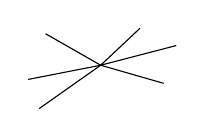
\begin{tikzpicture}[x=1cm,y=1cm,baseline=0cm]
\draw (-0.7,0.4) -- (0,0) -- (0.8,-0.23);
\draw (-0.92,-0.18) -- (0,0) -- (0.96,0.25);
\draw (-0.78,-0.55) -- (0,0) -- (0.5,0.47);
\end{tikzpicture}
\end{adjustbox}

Соотв. решётка содержит 28 элементов

$k=4$ долго (Гельф. и Пономарев): формулировку см. в кн. Манина
[Под строкой: по логике]

Рассм. $r$ элементов $e_1,\ldots,e_r$ и свободная модулярная
решетка, порожденная
[Зачёркнуто: \Incomplete{GELFAND-P001326}{generators-deletion}{Короткая запись перед «этими буквами» не читается.}]
этими буквами.
\Unclear{GELFAND-P001326}{generator-count}{Буква числа образующих и последнего индекса: $r$ / $\tau$.}

(см. Биркгоф, "Теория структур")

операции: сумма $+$ и пересеч. $\cdot$

равные — если по аксиомам преобразуются

$r\geq5$: зад. о тожд. слов неразрешима

Предст. $x\rightsquigarrow\underset{\text{подпр-во}}{\varrho(x)}\subset V$

\begin{equation*}
\varrho(x_1x_2)=\varrho(x_1)\cap\varrho(x_2),\qquad
\varrho(x_1+x_2)=\varrho(x_1)+\varrho(x_2)
\end{equation*}

\underline{\Unclear{GELFAND-P001326}{student-surname}{Рыжкова}}
(дипломница Семенова): можно ли конечным числом аксиом
сформулир. линейную эквивалентность?

Пусть есть 2 предст. $\varrho_j$ в $V_j$, $j=1,2$.

Морфизм $\varphi$ — лин. отобр. $\varphi:V_1\to V_2$, если
$\varphi(\varrho_1(x))\subset\varrho_2(x)$.

Неразложимое предст. — если $V_{\varrho}$ не раскл. в прям. сумму \ldots
\Unclear{GELFAND-P001326}{indecomposable-subscript}{Густо обведённый нижний знак при $V$: $\varrho$.}

Предст. $\varrho$ наз. \underline{предпроективным}, если $\forall$ неразложимого предст. $\varrho(x)$

\Unclear{GELFAND-P001326}{bottom-continuation}{На этом видимая запись обрывается; продолжение в назначенных кадрах отсутствует.}
\SourcePage{GELFAND-P001327}{unlabelled}
$\exists$ лишь конечное число \Unclear{GELFAND-P001327}{upper-line-noun}{наддувов} $\tau\colon\rho\longrightarrow\rho_0$

По Арнольду — это предст. без параметров.

Эл. реш. наз. \underline{препроективно эквив.}, если их не различает ни одно
препроект. предст.

Отождествляем — получим редукцию.

\underline{Задача} (будет сделана) [Под строкой: реально уже сделана]; найти ред. свободной решётки.

\underline{Теор. 1.} \underline{Все препроективные предст.} [Вставлено над строкой: своб.] \underline{реш. с $\Unclear{GELFAND-P001327}{theorem-one-generator}{r}$ \Unclear{GELFAND-P001327}{theorem-one-abbreviation}{обру.} описаны.}

\underline{Теор. 2.} \underline{Препроективные предст. решётки и её редукции совпадают.}

\underline{Опр.} Эл. $a$ реш. наз. \underline{совершенным}, если $\forall$ предст. [Вставлено над строкой: (в пр-ве $V$)] либо
\begin{equation*}
\rho(a)=V\ \text{либо}\ \rho(a)=0
\end{equation*}
(это аналог центра групп. кольца)

Соверш. элементы можно описать.

\SourcePage{GELFAND-P001328}{unlabelled}
\underline{24/XI-86 г.}\qquad \underline{Сем. Гельфанда}

\underline{Зелевинский А.}\qquad \underline{Неприводимые представления $GL(n,\mathbb{C})$}
(по раб. \Unclear{GELFAND-P001328}{header-source-name}{Тадича} и Вогана)

Рассм. предст. группы $GL(n,\mathbb{C})$; мн-во непр. унит. предст. обозн.: $GL(n,\mathbb{C})^{\wedge}$.
[Перед надстрочным $\wedge$ зачёркнут знак: \Unclear{GELFAND-P001328}{dual-cancellation}{$u$}.]

[Вставлено слева над строкой: Теперь] Изв. все унитарные представления этой группы.

(доказано, что найденные

\begin{equation*}
D^u=(\text{мультипл. хар-ры поля }\mathbb{C}),\quad \text{т.е. }D^u\ni\delta\colon
\end{equation*}
\begin{equation*}
\text{(1)}\qquad \delta(z)=\left(\frac{z}{|z|}\right)^k|z|^{i\rho},\quad k\in\mathbb{Z},\ \rho\in\mathbb{R}
\end{equation*}
\begin{equation*}
\text{(2)}\qquad u(\delta,n)(g)=\delta(\det g)\quad\text{— унитарное предст. }GL(n,\mathbb{C}).
\end{equation*}

Доп. семейство представлений
[Слева от следующих двух строк проведена двойная вертикальная черта.]
\begin{equation*}
\pi(u(\delta,n),\alpha),\qquad 0<\alpha<\frac12
\end{equation*}
предст. $GL(2n,\mathbb{C})$ (параб. индуцирование)

\begin{center}
\begin{adjustbox}{max width=\linewidth}
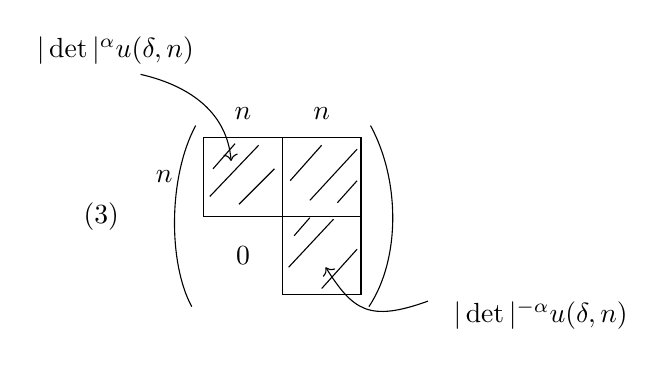
\begin{tikzpicture}[x=1cm,y=1cm]
\node at (-1.3,1) {(3)};
\draw (0,1) rectangle (1,2);
\draw (1,2)--(2,2)--(2,1)--(1,1);
\draw (1,0) rectangle (2,1);
\draw (0.08,1.25)--(0.7,1.9);
\draw (0.12,1.6)--(0.4,1.92);
\draw (0.45,1.15)--(0.9,1.6);
\draw (1.1,1.45)--(1.5,1.9);
\draw (1.35,1.2)--(1.95,1.85);
\draw (1.7,1.17)--(1.95,1.45);
\draw (1.08,0.35)--(1.65,0.96);
\draw (1.15,0.75)--(1.35,0.98);
\draw (1.5,0.08)--(1.95,0.58);
\draw (-0.1,2.15)..controls (-0.45,1.5) and (-0.45,0.4)..(-0.15,-0.15);
\draw (2.12,2.15)..controls (2.5,1.45) and (2.5,0.45)..(2.1,-0.15);
\node at (0.5,0.5) {$0$};
\node at (0.5,2.3) {$n$};
\node at (1.5,2.3) {$n$};
\node at (-0.5,1.5) {$n$};
\node[anchor=east] at (0,3.1) {$|\det|^{\alpha}u(\delta,n)$};
\draw[->] (-0.8,2.8)..controls (-0.15,2.65) and (0.3,2.3)..(0.35,1.7);
\node[anchor=west] at (3.05,-0.25) {$|\det|^{-\alpha}u(\delta,n)$};
\draw[->] (2.85,-0.08)..controls (2.1,-0.35) and (1.9,-0.2)..(1.55,0.35);
\end{tikzpicture}
\end{adjustbox}
\end{center}

и $\pi$ — индуц. этим 1-мерным представлением.
\begin{equation*}
\text{(4)}\qquad\pi(u(\delta,n),\alpha)=\operatorname{Ind}^{GL(2n,\mathbb{C})}
\end{equation*}

И.М.Г. \underline{Опред. индуц. предст.}\qquad $G\supset H$, $\pi(h)$ задано

Рассм. ф-и $f(g)$ на гр. $G$ со знач. в пр-ве предст. $\pi$, такие что $f(hg)=\pi(h)f(g)$

\SourcePage{GELFAND-P001329}{42}
В пр-ве таких ф-й действует $G$ и это предст. наз.
индуцированным.

Функтор ограничения двойственен функтору индуцирования.

\underline{3.} Любое представление [Вставлено под строкой: (непр. унит.)] получается из этих след. образом

Рассм. набор $(n_1,\ldots,n_k)$, $n_1+n_2+\ldots+n_k=n$ и набор
$\sigma_i\in GL(n_i,\mathbb{C})^{\vee}$ одного из 2-х опис. видов

\begin{center}
\begin{adjustbox}{max width=\linewidth}
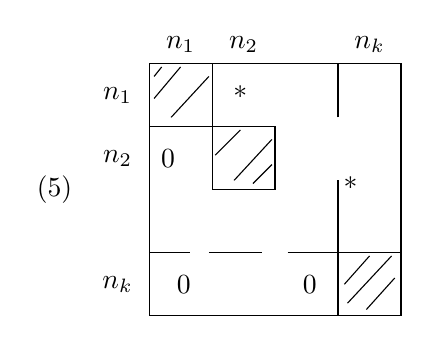
\begin{tikzpicture}[x=0.8cm,y=0.8cm]
\node at (-1.5,2) {(5)};
\draw (0,0) rectangle (4,4);
\draw (0,3)--(1,3)--(1,4);
\draw (1,2) rectangle (2,3);
\draw (3,0)--(3,1)--(4,1);
\draw (3,3.15)--(3,4);
\draw (3,1)--(3,2.15);
\draw (0,1)--(0.65,1);
\draw (0.95,1)--(1.8,1);
\draw (2.2,1)--(3,1);
\draw (0.08,3.45)--(0.5,3.95);
\draw (0.08,3.8)--(0.2,3.95);
\draw (0.35,3.15)--(0.95,3.8);
\draw (1.05,2.55)--(1.45,2.95);
\draw (1.35,2.15)--(1.95,2.8);
\draw (1.65,2.1)--(1.95,2.4);
\draw (3.1,0.5)--(3.5,0.95);
\draw (3.15,0.2)--(3.85,0.95);
\draw (3.45,0.1)--(3.9,0.6);
\node at (1.45,3.55) {$\ast$};
\node at (3.2,2.1) {$\ast$};
\node at (0.3,2.5) {$0$};
\node at (0.55,0.5) {$0$};
\node at (2.55,0.5) {$0$};
\node at (0.5,4.3) {$n_1$};
\node at (1.5,4.3) {$n_2$};
\node at (3.5,4.3) {$n_k$};
\node at (-0.5,3.5) {$n_1$};
\node at (-0.5,2.5) {$n_2$};
\node at (-0.5,0.5) {$n_k$};
\end{tikzpicture}
\end{adjustbox}
\end{center}

Рассм. для такой гр. предст. $\bigotimes\sigma_i$ и индуцируем.

\underline{Теорема}

а) Получ. непривод. и унитарное;

б) $\forall$ непр. унит. им. такой вид

в) эквив. $\Longleftrightarrow$ $\sigma_i$ отлич. перестановкой

\begin{center}— . —\end{center}

$D^u$ = квадр. интегр. представления груп. $GL(k,F)$ для нек-ро $k$

(с квадр. интегр. матр. элементами).

Тогда формулир. теор. (5) остаётся верной $\forall$ поля.

(Раньше было $k=1$.)

\begin{equation*}
u(\delta,n)\in GL(nk,F)^{\wedge}
\end{equation*}

\begin{center}
\begin{adjustbox}{max width=\linewidth}
\begin{tikzpicture}[x=0.85cm,y=0.85cm]
\node at (-1.05,1.3) {(6)};
\draw (0,2)--(0.75,2)--(0.75,2.8);
\draw (0.75,1.2) rectangle (1.55,2);
\draw (1.55,0.4) rectangle (2.35,1.2);
\draw (-0.1,2.85)..controls (-0.85,1.4) and (-0.85,-0.1)..(-0.3,-0.5);
\draw (3.7,2.6)..controls (4.1,1.7) and (4.05,0.3)..(3.65,-0.15);
\node at (0.3,2.45) {$\delta$};
\node at (0.3,1.55) {$0$};
\node at (0.3,0.7) {$0$};
\node at (1.1,0.7) {$0$};
\node at (1.15,2.4) {$\ast$};
\node at (2.6,2.1) {$\ast$};
\node at (0.35,3.2) {$k$};
\node at (1.2,3.2) {$k$};
\node at (2.65,3.2) {$\cdots$};
\node at (4.4,3.2) {$k$};
\node at (-0.5,2.45) {$k$};
\node at (-0.7,1.55) {$k$};
\node[anchor=west] at (5.35,2.3) {$\nu^{\frac{n-1}{2}}\delta\otimes\nu^{\frac n2-1}\delta\ \ldots\ \otimes\nu^{-\frac{n-1}{2}}$};
\draw[->] (5.15,2.3)--(4.3,1.8);
\node[anchor=west] at (-0.3,-1.15) {$u(\delta,n)$ — единств. непривод. фактор представления $\operatorname{Ind}(\ldots)$};
\draw[->] (12.7,-0.85)..controls (13.2,-0.1) and (12.8,0.55)..(12,0.85);
\end{tikzpicture}
\end{adjustbox}
\end{center}
[Показатель у второго $\nu$ вставлен над зачёркнутым: \Unclear{GELFAND-P001329}{second-exponent-cancellation}{неразборчиво}.]

\underline{Вопрос И.М.Г.:} как с другими группами?

\underline{Кириллов}
[Рядом зачёркнуто: \Unclear{GELFAND-P001329}{kirillov-cancellation}{Кир.}]

\underline{Кроме} $GL(n,\mathbb{C})$ \underline{известны ещё все унит. неприв. предст. групп}
\begin{equation*}
b_2=C_2\ ;\qquad G_2\ ;\qquad SU(2,2)\ ;\qquad SU(2,n)
\end{equation*}
\begin{equation*}
SO(5)\sim Sp(4)\qquad\qquad\text{Knapp}
\end{equation*}
(Дюфло)

Кватернионные сделал Vogan

\begin{center}
\begin{adjustbox}{max width=\linewidth}
\begin{tikzpicture}[x=0.75cm,y=0.75cm]
\node[anchor=east] at (-0.55,0.8) {ответ $\approx$};
\draw (0,0)--(0,1)--(1,1)--(1,2.7);
\draw (-0.65,0)--(1,0)--(1,1)--(2.55,1);
\draw (0,-0.75)--(0,0);
\draw (0.05,0.3)--(0.7,0.95);
\draw (0.05,0.7)--(0.3,0.95);
\draw (0.25,0.1)--(0.9,0.75);
\draw (0.7,0.05)--(0.95,0.3);
\draw (1.02,2.1)--(1.55,2.65);
\draw (1.1,1.55)--(2,2.5);
\draw (1.15,1.15)--(2.3,2.15);
\draw (1.65,1.05)--(2.45,1.75);
\draw (2.2,1.05)--(2.55,1.4);
\fill (-1,-0.15) circle (0.045);
\fill (-0.75,-0.38) circle (0.045);
\fill (-0.5,-0.61) circle (0.045);
\fill (-0.25,-0.82) circle (0.045);
\end{tikzpicture}
\end{adjustbox}
\end{center}

\SourcePage{GELFAND-P001330}{unlabelled}
\underline{И.М.Г.} Введем скал. произвед
\begin{equation*}
\int |x_1-x_2|^{-\varrho} f(x_1)\overline{f(x_2)}\,dx_1dx_2
\end{equation*}
При $\varrho<2$ интеграл сходится

$\varrho>2\Rightarrow$ надо аналит. продолжать и форма не будет полож. опред.
\begin{equation*}
\int t^{\widetilde{\varrho}}
\left|\varphi(t)\right|^2\,dt
\end{equation*}
[В обозначении функции $\varphi$ написана поверх \Unclear{GELFAND-P001330}{upper-overwritten-function}{$f$?}.]
Полож. при $\varphi(0)=0$, а иначе (регуляризация) надо еще наложить усл. $\varphi'(0)=0$ и т.д.

Степень расход. $\to$ число минусов

\underline{\underline{Казаков.}}

\underline{Интегралы, к-ые надо сосчитать}
\begin{equation*}
\int d(\Omega)_{U(N)}\exp[\operatorname{tr}\Omega^+p^\mu\Omega p^\mu],\qquad \Omega^+=\Omega^{-1}
\tag{1}
\end{equation*}
[Над второй $\Omega$ зачеркнуто: \Unclear{GELFAND-P001330}{integral-one-cancelled-superscript}{знак $+$?}]
\begin{equation*}
p^\mu=\operatorname{diag}(p_1^\mu,p_2^\mu,\ldots,p_N^\mu),\quad \mu=1,2
\end{equation*}
Интересно и обобщение
\begin{equation*}
\int d(\Omega)_{U(N)}\exp[\operatorname{tr}(\Omega^{-1}p^\mu\Omega q^\mu)].
\tag{2}
\end{equation*}
Без $\mu$: 1-мерное [зачеркнуто: \Unclear{GELFAND-P001330}{one-dimensional-cancellation}{кр.?}] кир. поле (трив. задача)

$\mu=1,2$: 2-мерное кир. поле (не вычислен)
\begin{equation*}
\downarrow
\end{equation*}
сделано другим способом.

По теории возмущ. показывается, что воспроизв. все [вставлено над строкой: планарные] диаграммы
2-мерн. кир. поля. А именно, пишем
\begin{equation*}
\Omega=e^{iA}
\tag{3}
\end{equation*}
и разлаг. по степеням $A$.

Приближение: $\Omega=1$, а потом учит. флуктуации.
\begin{equation*}
(2)=Z(p,q)
\tag{4}
\end{equation*}
Надо напис. меру Хаара и в $d\Omega$ тоже подст. $\Omega=e^{iA}$.

В главном пор. --- гауссов член.

[У правого края кадра, за вертикальной границей листа: \Unclear{GELFAND-P001330}{right-edge-fragments}{обрезанная скобка; фрагмент «(6»; обрезанная скобка}.]

\SourcePage{GELFAND-P001331}{43}
\begin{equation*}
Z=\int\prod_{\mu=1}^{d}d(\Omega_\mu)\exp\left[\beta\sum_{\mu,\nu}\operatorname{tr}\Omega_\mu\Omega_\nu\Omega_\mu^+\Omega_\nu^+\right]
\tag{5}
\end{equation*}
Это эквив. обычной калибр. теории (как ф-и от $\beta$) при $N\to\infty$.
\begin{center}
--- $\cdot$ ---
\end{center}
\underline{Вычисление интегралов}
\begin{equation*}
F(c,g)=\lim_{N\to\infty}\frac{1}{N^2}\log\int d^{N^2}u\,d^{N^2}v\,
\exp\operatorname{tr}\left(-u^2-v^2+2cuv-\frac{g}{N}(u^4+v^4)\right),
\tag{6}
\end{equation*}
\begin{equation*}
u^+=u,\quad v^+=v
\end{equation*}
[Два коротких горизонтальных штриха над словом «графов».]

$F(c,g)$ --- производ. ф-я графов --- покрытий сферы 4-угольниками

\begin{center}
\begin{adjustbox}{max width=\linewidth}
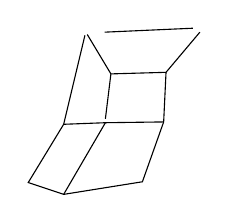
\begin{tikzpicture}[scale=1]
\draw (0.65,2.05)--(0.95,1.55)--(1.65,1.57)--(2.08,2.08);
\draw (0.87,2.08)--(1.99,2.13);
\draw (0.62,2.04)--(0.35,0.91)--(-0.10,0.17)--(0.35,0.02)--(1.35,0.18)--(1.62,0.94)--(1.65,1.57);
\draw (0.95,1.55)--(0.88,0.98);
\draw (0.35,0.91)--(0.88,0.93)--(1.62,0.94);
\draw (0.88,0.93)--(0.35,0.02);
\end{tikzpicture}
\end{adjustbox}
\end{center}
Все 4-уг. раскрашены в 2 цвета (белые и черные)
\begin{equation*}
F(c,g)=\sum T_n^m g^n\quad [\text{зачеркнуто: }\exp]\quad e^{2cm}
\end{equation*}
$T_n^m$ --- число графов, у к-ых длина границы [зачеркнуто: \Unclear{GELFAND-P001331}{graph-definition-cancellation}{раскрашенных?}]
раскрашенных пятен равна $m$; $n$ --- число квадратиков

(длина ребра $\overset{\mathrm{def}}{=}1$)

Это же эквив. \underline{модели} \underline{Изинга}. $\nearrow$

Пусть
\begin{equation*}
u=\Omega_1^+\lambda\Omega_1,\quad v=\Omega_2^+\mu\Omega_2,
\qquad \lambda,\mu\text{ --- диагон. матрицы}
\end{equation*}
Тогда
\begin{equation*}
\begin{aligned}
F(c,g)={}&\lim_{N\to\infty}\frac{1}{N^2}\log\iint
\left(\prod_{i=1}^{N}d\lambda_i\,d\mu_i\right)\Delta^2(\lambda)\Delta^2(\mu)
\exp\left[-\sum_{i=1}^{N}\left[\lambda_i^2+\mu_i^2+\frac{g}{N}(\lambda_i^4+\mu_i^4)\right]\right]\\
&\int d\Omega\,\exp 2c\operatorname{tr}(\Omega^+\lambda\Omega\mu),
\end{aligned}
\tag{7}
\end{equation*}
[Перед формулой справа отдельный знак: \Unclear{GELFAND-P001331}{relative-angle-mark}{4 или исправленная стрелка}.]
\begin{equation*}
\underbrace{\Omega=\Omega_1\Omega_2^+}_{\substack{\text{относит. матр.}\\\text{угл.}}}
\end{equation*}
здесь $\Delta(\lambda)=\prod_{i<j}(\lambda_i-\lambda_j)$

Но:
\begin{equation*}
\int d\Omega\,\exp 2c\operatorname{tr}(\Omega^+\lambda\Omega\mu)
=\Unclear{GELFAND-P001331}{unitary-integral-normalization}{\frac{\det e^{2c\lambda_i\mu_j}}{\Delta(\mu)\Delta(\lambda)}}
\tag{8}
\end{equation*}
Переменных уже $2N$ и действует метод перевала!

[Зачеркнуто: Автоматиче] Получим
\begin{equation*}
\begin{aligned}
F(c,g)={}&\lim_{N\to\infty}\frac{1}{N^2}\log\int\prod_1^N d\lambda_i\,d\mu_i\,\Delta(\lambda)\Delta(\mu)\times\\
&\underbrace{\times\exp\left[-\sum_1^N\left[\lambda_i^2+\mu_i^2+\frac{g}{N}(\lambda_i^4+\mu_i^4)-2c\lambda_i\mu_i\right]\right]}_{\Unclear{GELFAND-P001331}{weight-brace}{w(\lambda_i,\mu_i)}}
\end{aligned}
\tag{9}
\end{equation*}
$\Delta(\lambda)$ антисимм., $\Rightarrow$ автом. происходит антисимметризация

\SourcePage{GELFAND-P001332}{unlabelled}
\begin{equation*}
F(c,g)=\lim_{N\to\infty}\frac{1}{N^2}\log\iint\prod_{i=1}^{N}d\lambda_i\,d\mu_i\,w(\lambda_i,\mu_i)\Delta(\lambda)\Delta(\mu).
\tag{10}
\end{equation*}
Есть полиномы, ортог. с весом $W$ и с высше. \Unclear{GELFAND-P001332}{monic-text}{мерой?}
\begin{equation*}
\Delta(\lambda)=\det(\lambda_i^{j-1})_{i,j=1}^{N}=\det[P_{j-1}(\lambda_i)],
\tag{11}
\end{equation*}
где
\begin{equation*}
P_j(\lambda)=\lambda^j+\sum_{k=0}^{j-1}a_k\lambda^k
\end{equation*}
[В аргументе $P_j$ буква $\lambda$ написана поверх \Unclear{GELFAND-P001332}{polynomial-argument-overwrite}{$z$?}.]

\Unclear{GELFAND-P001332}{orthogonal-opening-mark}{И?} Сист. ортог. полиномов $P_j$ строим так, что
\begin{equation*}
\int_{-\infty}^{\infty}d\lambda\,d\mu\,W(\lambda,\mu)P_i(\lambda)P_j(\mu)=h_i\delta_{ij}
\tag{12}
\end{equation*}
Тогда
\begin{equation*}
\Unclear{GELFAND-P001332}{polynomial-determinant}{P_j(\lambda)=\det\begin{pmatrix}
m_{00}&m_{01}&\cdots&&m_{0i}\\
m_{10}&\cdot&\cdot&\cdot\ \cdot&m_{1i}\\
1&\lambda&\lambda^2&\cdots&\lambda^i
\end{pmatrix}},
\tag{13}
\end{equation*}
где
\begin{equation*}
m_{ij}=\int d\lambda\,d\mu\,w(\lambda,\mu)\lambda^i\mu^j.
\tag{14}
\end{equation*}
На $h_j$ получ. система рекурр. ур-й, в пределе беск. $N$ оказ.
одним ур-ем. Далее,
\begin{equation*}
\iint\prod d\lambda_i\,d\mu_i\,w(\lambda_i,\mu_i)\Delta(\lambda)\Delta(\mu)
=\Unclear{GELFAND-P001332}{norm-product}{\prod_{i=1}^{N}h_i}
\tag{15}
\end{equation*}
Ответ:
\begin{equation*}
\left\{\begin{aligned}
F(c,z)&=\frac{1}{2}\ln\frac{z}{g(z)}+\frac{1}{2g^2(z)}\int_0^z\frac{dt}{t}g^2(t)-\frac{1}{g(z)}\int_0^z\frac{dt}{t}g(t)\\
g\ \text{[зачеркнуто: }\Unclear{GELFAND-P001332}{coupling-cancelled-argument}{(z)\text{?}}\text{]}&=\frac{z}{(1-3z)^2}-c^2z+3c^2z^3
\end{aligned}\right.
\tag{16}
\end{equation*}
Исключая отсюда $z$, получим $F(c,g)$.

(это параметрич. задание ответа)

Это позволяет изучить асимптотику числа графов

([зачеркнуто: \Unclear{GELFAND-P001332}{conclusion-cancellation}{неразборчивый знак}] используем $g'_z(z)=0$ --- особенности)

\SourcePage{GELFAND-P001333}{unlabelled}
\underline{9.2.87г.}\qquad \underline{\underline{Сем. Гельфанда.}}

\underline{\underline{Дон Цагир (Don Zagier)}}

\underline{И.М.Г.} Идея Фалтинга: делать $p$-адич. струны.

Одна работа (задача к след. семинару) Don Zagier.
Дан ориентированный $2N$-угольник, стороны разб. на пары
(каждая склеена с какой-то)
[Вставка над строкой: с самой-собой нельзя]

Отожд. наоборот (со сменой ориентации)
Получ. поверхность рода $g$

\SourceFigure{GELFAND-P001333}{polygon-gluing}{Слева шестиугольник: верхняя и нижняя стороны почти горизонтальны, четыре боковые стороны наклонены. На контуре стрелки; внутри две пересекающиеся прерывистые кривые со стрелками к сторонам. Точное направление части коротких стрелок и их соединение с контуром требуют проверки по источнику.}

[На левом поле:]
\begin{adjustbox}{max width=\linewidth}
\begin{tikzpicture}[baseline=(current bounding box.center)]
\draw (0,0.65) ellipse (0.28 and 0.45);
\node at (0,0.65) {!};
\draw (0,-0.15) ellipse (0.7 and 0.3);
\node at (0,-0.15) {конкурс};
\end{tikzpicture}
\end{adjustbox}

Сколько есть способов склейки, чтобы получилась пов. рода $g$?

Написать ф-лу. (2 способа, отлич. поворотом, считаются разными)
(ф-я от $N$ и $g$).

\begin{adjustbox}{max width=\linewidth}
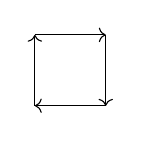
\begin{tikzpicture}[baseline=(current bounding box.center)]
\draw[->] (0,0) -- (0,0.9);
\draw[->] (0,0.9) -- (0.9,0.9);
\draw[->] (0.9,0.9) -- (0.9,0);
\draw[->] (0.9,0) -- (0,0);
\end{tikzpicture}
\end{adjustbox}
можно получить тор и сферу.

Это основа для вычисл. \underline{эйлеровой} хар-ки пр-ва Тейхмюллера!

\underline{D.Z.}\qquad 2 вещи.
\underline{Модулярные формы и специальные значения дзета-функций}

1. Classical Modular forms

2. Special values of zeta-functions

Modular forms. (\underline{parabolic})

\begin{equation*}
\Gamma=SL(2,\mathbb Z)/\{\pm1\},\qquad
H=\{z=x+iy;\ y>0\}
\end{equation*}

$f(z)$ голом. [вставлено над строкой: на $H$],
[зачёркнуто: \Unclear{GELFAND-P001333}{cusp-cancellation}{$O(1)$?}; над зачёркнутым: нуль]
на $\infty$ и

\begin{equation*}
f\left(\frac{az+b}{cz+d}\right)=(cz+d)^k f(z)
\tag{1}
\end{equation*}
\begin{equation*}
a,b,c,d\in\mathbb Z,\qquad
ad-bc=\Unclear{GELFAND-P001333}{determinant-sign}{\pm1}
\end{equation*}

[Справа:]
Нуль на $\infty$ — cusp.
\begin{equation*}
S_k=\{f\},\qquad \dim S_k<\infty
\end{equation*}

\SourcePage{GELFAND-P001334}{69}
Hecke: $\exists$ many

\begin{equation*}
f(z)=\sum_{n=1}^{\infty}a(n)e^{\Unclear{GELFAND-P001334}{fourier-exponent-sign}{-2\pi inz}}
\tag{2}
\end{equation*}
(т.к. из (1) следует, что $f(z+1)=f(z)$)

$\exists$ база, в к-рой $a(n)\in\mathbb Z$

(3) \underline{Пример.}

При $k=2,4,6,8,10,14$ $S_k=\{0\}$ (нет параб. форм)

\underline{Модулярная форма:} $O(1)$ на $\infty$ (а не нуль)

\begin{equation*}
M_k\ni f(z)=\sum_{n=0}^{\infty}a(n)q^n,\qquad q=e^{2\pi iz}
\tag{4}
\end{equation*}

Тогда $\exists$ ряд
[зачёркнуто: \Unclear{GELFAND-P001334}{eisenstein-cancellation}{E\ldots}]
Eisenstein'a

\begin{equation*}
E_k(z)=\frac12\sum_{(c,d)=1}\frac{1}{(cz+d)^{\Unclear{GELFAND-P001334}{eisenstein-exponent}{2}}}
\tag{5}
\end{equation*}

\underline{Упр.:} проверить
[зачёркнуто: \Unclear{GELFAND-P001334}{automorphy-cancellation}{его / это}]
автоморфность.

\begin{align*}
E_4(z)&=1+240(q+9q^2+28q^3+73q^4+\ldots)=\tag{6}\\
&=1+240\sum_{n=1}^{\infty}
\underbrace{\sigma_3(n)}_{\substack{\Vert\\\sum_{d\mid n}d^3}}q^n
\end{align*}

(7) $k$ нечётно $\Rightarrow$ нет параболич. форм (очевидно из знаков)

\begin{equation*}
S_k\ni\Delta(z)=q-24q^2+252q^3+\ldots-6048q^6+\ldots
=\sum\tau(n)q^n
\tag{8}
\end{equation*}
(нет пост. ч. $\Rightarrow$ параб.

\begin{equation*}
24\cdot252=6048
\end{equation*}

\begin{equation*}
\tau(nm)=\tau(n)\tau(m)\quad\text{при }(n,m)=1.
\tag{9}
\end{equation*}

(10) \underline{\underline{Утв.}} $\exists$ базис параб. форм, у к-рых коэфф. облад. св-вом (9)

\begin{equation*}
\frac{E_4}{240}=\frac{1}{240}+\sum_{n=1}^{\infty}\sigma_3(n)q^n,
\qquad \sigma_3(6)=\sigma_3(2)\sigma_3(3)
\tag{11}
\end{equation*}

(12) \underline{Опр.} $f(z)$ наз. формой Гекке (Hecke), если
\begin{equation*}
f=\sum_0^{\infty}a(n)q^n
\end{equation*}
\begin{equation*}
a(nm)=a(n)a(m)\quad\text{при }(n,m)=1
\end{equation*}

(13) \underline{Утв.} Число форм Гекке $=$ разм. подпр-ва и они обр. базис.

\SourcePage{GELFAND-P001335}{unlabelled}
\underline{Д-во.} Опер. Гекке
$T_n\colon$
\begin{adjustbox}{max width=\linewidth}
\begin{tikzcd}
S_k \arrow[loop right]
\end{tikzcd}
\end{adjustbox}
;\quad
$\gamma=\begin{pmatrix}a&b\\c&d\end{pmatrix}$, $f=f(z)$.

(14) Обозначение:
\begin{equation*}
(f\mid\gamma)(z)=
\left(\frac{cz+d}{\sqrt{ad-bc}}\right)^{-k}
f\left(\frac{az+\Unclear{GELFAND-P001335}{slash-numerator}{b}}{cz+d}\right)
\qquad
\text{(действие }SL_2(R)\text{)}
\end{equation*}
[Под $cz+d$ вставлен знаменатель $\sqrt{ad-bc}$ и продлена скобка.]

[Справа под «действие $SL_2(R)$»:] и даже $GL_2^+(R)$.
\begin{equation*}
M_k\ni f\Longleftrightarrow f\mid\gamma=f
\qquad(\gamma\in\Gamma).
\end{equation*}
\begin{equation*}
T_1=1.
\end{equation*}
[Над $f$ в следующей формуле приписано $S_k$ со стрелкой вниз к $f$.]
\begin{equation*}
\tag{15}
T_n(f)(z)=
\Unclear{GELFAND-P001335}{hecke-normalization}{\frac{n^{\frac{k}{2}-1}}{2}}
\sum_{\gamma\in\Gamma\backslash M_n}f\mid\gamma.
\end{equation*}
\begin{equation*}
M_n\subset M(2,Z)
\quad\text{— }\underset{2\times2}{\text{матр.}}\text{ с }\det=n.
\end{equation*}
$n=2\Rightarrow$ есть 3 члена.
\begin{equation*}
\tag{16}
\begin{aligned}
T_2(f)&=2^{\frac{k}{2}-1}
\left[
f\mid\begin{pmatrix}2&0\\0&1\end{pmatrix}
+f\mid\begin{pmatrix}1&0\\0&2\end{pmatrix}
+f\mid\begin{pmatrix}1&1\\0&2\end{pmatrix}
\right]=\\
&=2^{k-1}f(2z)+\frac12f\left(\frac z2\right)
+\frac12f\left(\frac{z+1}{2}\right).
\end{aligned}
\end{equation*}
[У первого $f$ во второй строке зачёркнуты штрихи:
\Unclear{GELFAND-P001335}{hecke-cancelled-factor}{возможно, прежний знаменатель $2$}.]

\underline{Пример:} \underline{$k=12$}. Тогда для $\Delta$, зад. рядом Фурье,
\begin{equation*}
\tag{17}
T_2(\Delta)=2^{11}\sum_{n=1}^{\infty}\tau(n)q^{2n}
+\sum_{n=1}^{\infty}\tau(2n)q^n.
\end{equation*}
Из условия $T_2(\Delta)=\lambda_2\Delta$ находим
$\lambda_2=-24$ и т.\,д.

(18) Соб. знач. $\lambda_n$ всегда есть коэфф. Фурье
(просто получается).

(19) \underline{Опр. 2.} $f$ — форма Гекке
$\Longleftrightarrow T_n(f)=\lambda_nf$, $\forall n$.

Сущ. базиса вытек. из 2-х фактов:
\begin{equation*}
\tag{20}
\text{а) }\ T_nT_m=T_mT_n.
\end{equation*}
б) $S_k$ имеет скал. произв. (Petersson), в к-ром
$T_n$ самосопряжены!

Тогда $\exists$ базис общих соб. векторов.

Всегда:
\begin{equation*}
\tag{21}
\begin{gathered}
a(1)=1\\
a(n)=\lambda_n.
\end{gathered}
\end{equation*}
\begin{equation*}
\tag{22}
\underset{\text{при }(n,m)=1}{T_nT_m=T_{nm}}
\quad\Longrightarrow\quad a(n)a(m)=a(nm).
\end{equation*}
(\underline{Mordell} ввёл опер. Гекке в 1917 г.)

Гекке доказал импликацию (22).

\SourcePage{GELFAND-P001336}{70}
\underline{Вопрос:} вычислить $\operatorname{Tr}(T_n)$
\qquad $T_n\colon$
\begin{adjustbox}{max width=\linewidth}
\begin{tikzcd}
S_k \arrow[loop right]
\end{tikzcd}
\end{adjustbox}

\underline{$k=12$};\quad
$\displaystyle\Delta=\sum_1^\infty\tau(n)q^n$.
\begin{equation*}
\tag{23}
T_n(\Delta)=\tau(n)\Delta,\quad
T_n=(\tau(n)),\quad \operatorname{Tr}T_n=\tau_n.
\end{equation*}
Ф-ла следа даст, в частности, ф-лу для $\tau(n)$.

Скал. произв.:
\begin{equation*}
\tag{24}
(f,g)=\int_{\Gamma\backslash H}
f(z)\overline{g(z)}y^k
\underbrace{dV}_{\frac{dx\,dy}{y^2}\ (\text{инв. мера})},
\qquad f,g\in S_k.
\end{equation*}
([Над зачёркнутым словом вставлено $f(z)\overline{g(z)}y^k$ —;
зачёркнуто:
\Unclear{GELFAND-P001336}{invariance-cancellation}{оно / это}.]
$\Gamma$-инвариантно ($\Rightarrow$ интеграл имеет смысл).)

(25) \underline{Лемма.} Пусть $F(z)$ голом. на $H$ и дост. мала на
$\infty$, $k\geq2$, $z_0\in H$. Тогда
\begin{equation*}
\tag{26}
\int_H\frac{F(z)}{(\bar z-z_0)^k}y^k\,dV=C_kF(z_0),
\end{equation*}
где
\begin{equation*}
C_k=\frac{(-1)^{k/2}\pi}{2^{k-2}(k-1)}
\qquad\text{при }k\text{ чётном}.
\end{equation*}

\underline{Д-во.}
\begin{center}
\begin{adjustbox}{max width=\linewidth}
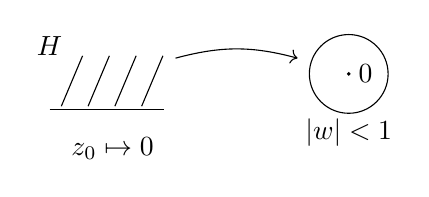
\begin{tikzpicture}
\node at (-0.25,0.8) {$H$};
\draw (-0.25,0) -- (1.2,0);
\draw (-0.1,0.04) -- (0.17,0.68);
\draw (0.24,0.04) -- (0.51,0.68);
\draw (0.58,0.04) -- (0.85,0.68);
\draw (0.92,0.04) -- (1.19,0.68);
\draw[->] (1.35,0.65) to[bend left=15] (2.9,0.65);
\draw (3.55,0.45) circle (0.5);
\fill (3.55,0.45) circle (0.025);
\node[right] at (3.55,0.45) {$0$};
\node at (3.55,-0.3) {$|w|<1$};
\node at (0.55,-0.5) {$z_0\mapsto0$};
\end{tikzpicture}
\end{adjustbox}
\end{center}
\begin{equation*}
w=\frac{z-z_0}{z-\bar z_0}=re^{i\theta},\quad 0\leq r<1,
\qquad z\in R\Rightarrow|w|=1.
\end{equation*}
Получим
\begin{equation*}
\int_0^1
\left[\int_0^{2\pi}\frac{G(w)}{(1-w)^k}\,d\theta\right]
\left(\frac{1-r^2}{\Unclear{GELFAND-P001336}{radial-factor}{2\pi}}\right)^{k-2}r\,dr.
\end{equation*}
$F(z)=G(w)$.
\begin{equation*}
\underbrace{\frac1i\int_{|w|=r}\frac{G(w)}{(1-w)^k}\frac{dw}{w}}_{=\,2\pi G(0)}
\qquad\triangleright
\end{equation*}
[От контурного интеграла проведена стрелка вверх к внутреннему интегралу
в квадратных скобках.]

\begin{equation*}
\tag{27}
K_n(\underset{\uparrow H}{z},\underset{\uparrow H}{z'})
=\frac12
\sum_{\begin{pmatrix}a&b\\c&d\end{pmatrix}\in M_n}
\frac{1}{[(cz+d)z'+(az+b)]^k}
\in S_k\otimes S'_k.
\end{equation*}
(ядро Бергмана)\qquad сход. при $k\geq4$.

[Справа внизу:]
\begin{equation*}
\left(
\text{т.\,к. }\ 
\frac{1}{(cz+d)^k}
\left(\frac{1}{z'+\frac{az+b}{cz+d}}\right)^k
\right)
\end{equation*}
\begin{equation*}
\Unclear{GELFAND-P001336}{kernel-slash-normalization}{=
\frac{1}{(z'+z)^k}\mid\gamma}.
\end{equation*}
% GELFAND-0145: diplomatic transcription of the ten assigned original PNG frames.
% Review coordinates below are original PNG pixels: left, top, right, bottom (right/bottom exclusive).
% scale records raster enlargement only; original scans remain authoritative.
% Review metadata is documentary and introduces no external TeX dependencies.
\SourcePage{GELFAND-P001337}{unlabelled}
% SourcePNG: images/GELFAND-P001337.png; sha256=85f31a8ee6627f8d02475f32e353463c2ef663661df04a846a5599c00409d4b2; dimensions=2408x3448
% ReviewCrop: {"region":"1337-eq28","bbox":[330,105,1740,338],"scale":3}
% ReviewCrop: {"region":"1337-lemma","bbox":[1220,365,1925,535],"scale":3}
% ReviewCrop: {"region":"1337-anyn","bbox":[340,550,1755,795],"scale":3}
% ReviewCrop: {"region":"1337-eq29","bbox":[370,1270,1740,1638],"scale":3}
% ReviewCrop: {"region":"1337-eq30","bbox":[300,1620,1460,1960],"scale":3}
% ReviewCrop: {"region":"1337-eq31","bbox":[140,1985,2160,2585],"scale":3}
% ReviewCrop: {"region":"1337-bottom","bbox":[335,2610,2150,3190],"scale":3}
% ReviewCrop: {"region":"1337-lemma-word","bbox":[1450,390,1655,510],"scale":6}
% ReviewCrop: {"region":"1337-eq28-cancel","bbox":[786,105,936,265],"scale":8}
% ReviewCrop: {"region":"1337-eq29-cancel","bbox":[724,1320,815,1440],"scale":8}
% ReviewCrop: {"region":"1337-fourier","bbox":[370,800,1620,1270],"scale":3}
% ReviewCrop: {"region":"1337-n1","bbox":[350,365,550,470],"scale":6}
% ReviewCrop: {"region":"cross-1337-conditional","bbox":[360,340,535,460],"scale":8}
% ReviewCrop: {"region":"1337-left-stroke","bbox":[105,2970,155,3065],"scale":8}
% ReviewCrop: {"region":"conditional","bbox":[360,340,535,460],"scale":8}
% ReviewCrop: {"region":"lemma-word","bbox":[1420,375,1695,520],"scale":6}
% ReviewCrop: {"region":"lower-margin","bbox":[105,2970,155,3065],"scale":6}
\begin{equation*}
\bigl(f(z),K_n(z,\bar z')\bigr)
=\int_{\Gamma\backslash H}\sum_{\gamma\in M_n}
\frac{f(z)}{(\bar z-z')^k}\mid\gamma\Bigr]y^k\,dV .
\tag{28}
\end{equation*}
[После знака интеграла зачёркнуто:]
\Unclear{GELFAND-P001337}{eq28-cancellation}{возможно, $\sum$; остальные штрихи неразборчивы.}

\begin{equation*}
n=1\quad\Rightarrow\quad\int_H\frac{f(z)}{(\bar z-z')^k}\,dz
\end{equation*}
\Unclear{GELFAND-P001337}{n-one-condition}{Первая буква условия густо обведена: $n$ или $k$ (возможно $\kappa$).}
и надо использ. лемму.

Любое $n$ $\Rightarrow$ получим $n^{1-k}C_kT_n(f)(z)$, т.е.
$K_n$ --- ядро опер. Гекке.

$f_1,\ldots,f_d$ --- базис форм Гекке в $S_k$
\begin{equation*}
f(z)=\sum_{n=1}^{\infty}a_j(n)q^n,
\end{equation*}
\begin{equation*}
a_j(1)=1,\qquad T_n(f_j)=a_j(n)f_j
\end{equation*}
\begin{equation*}
K_n(z,z')=\frac{C_k}{n^{k-1}}\sum_{j=1}^{d}
\frac{a_j(n)}{(f_j,f_j)}f_j(z)f_j(z')
\tag{29}
\end{equation*}
[После знака равенства, перед дробью, зачёркнуто:]
\Unclear{GELFAND-P001337}{eq29-cancellation}{возможно, $\sum$; знак закрыт штриховкой.}

(очевидно из-за диагональности матрицы)

\begin{equation*}
\int_{\Gamma\backslash H}K_n(z,-\bar z)y^k\,dV
=\frac{C_k}{n^{k-1}}\underbrace{\sum_{j=1}^{n}\lambda_j(n)}_{=\operatorname{Tr}T_n}
\tag{30}
\end{equation*}
\Unclear{GELFAND-P001337}{eq30-upper-limit}{Верхний предел суммы: $n$ [так в рукописи].}

Но:
\begin{align*}
K_n(z,-\bar z)
&=\frac12\sum_{\begin{pmatrix}a&b\\c&d\end{pmatrix}\in M_n}
\frac{1}{[c|z|^2+d\bar z-az-b]^k}\\
&=\sum_{t\in\mathbb Z}\sum_{\substack{Q\\\operatorname{disc}Q=t^2-4n}}
\frac{1}{(A|z|^2+Bx+C-ity)^k}
\tag{31}
\end{align*}
\Unclear{GELFAND-P001337}{eq31-coefficient}{Во второй строке перед суммой множитель $1/2$ не написан.}

[Слева от перехода ко второй строке:]
Положим
\begin{equation*}
\begin{aligned}
d+a&=t\\
c&=A\\
d-a&=B\\
-b&=C
\end{aligned}
\end{equation*}
[Под $t\in\mathbb Z$:] след

\begin{equation*}
Q=[A,B,C]=Au^2+Buv+Cv^2
\end{equation*}
\begin{align*}
\operatorname{disc}Q&=t^2-4n=B^2-4AC=\\
&=(d-a)^2+4bc=(d+a)^2-4(ad-bc)
\end{align*}

[На левом поле напротив вычисления дискриминанта --- отдельный короткий вертикальный штрих.]

$K_n(z,-\bar z)y^k$ должна быть $\Gamma$-инвариантна!

\SourcePage{GELFAND-P001338}{71}
% SourcePNG: images/GELFAND-P001338.png; sha256=c6c1c1e932409a0186dcf80866c663ef5d19b461f6484b9ebc3421b170315aa7; dimensions=2408x3448
% ReviewCrop: {"region":"1338-eq32-notes","bbox":[730,135,2145,750],"scale":3}
% ReviewCrop: {"region":"1338-theorem","bbox":[65,2880,2340,3435],"scale":3}
% ReviewCrop: {"region":"1338-middle","bbox":[235,805,1725,2210],"scale":3}
% ReviewCrop: {"region":"1338-eq36","bbox":[65,2280,2250,2870],"scale":3}
% ReviewCrop: {"region":"1338-name-cancel","bbox":[605,2890,935,3010],"scale":5}
% ReviewCrop: {"region":"1338-eq34-cancel","bbox":[1580,1635,1725,1760],"scale":7}
% ReviewCrop: {"region":"1338-eq36-index","bbox":[1080,2435,1190,2580],"scale":10}
% ReviewCrop: {"region":"1338-eq32-condition","bbox":[1520,580,2155,740],"scale":5}
% ReviewCrop: {"region":"1338-discriminant-abbrev","bbox":[1080,395,1265,545],"scale":6}
Получаем
\begin{equation*}
K_n(z,-\bar z)y^k=\sum_{t\in\mathbb Z}H(t^2-4n)(\cdot\,\cdot\,\cdot\,\cdot),
\tag{32}
\end{equation*}
[Стрелка к $H$:] число кв. форм с данным дискр. (class number)

[Стрелка к скобкам с точками:]
$=0$ при $t^2-4n>0$ или $\ne\square$
(не явл. точн. квадратом)
\Unclear{GELFAND-P001338}{eq32-vanishing-condition}{Связка условий: «или» [так в рукописи].}

а это уже конечная сумма!

\begin{equation*}
Q=[A,B,C],\qquad A,B,C\in\mathbb Z
\end{equation*}
\begin{equation*}
Au^2+Buv+Cv^2
\end{equation*}
$\Gamma$ действует:
\begin{equation*}
(Q\circ\gamma)(u,v)=Q\bigl((u,v)\gamma\bigr)
\end{equation*}
[Под словом «действует»:] на мн-ве таких $Q$

Для $t\in\mathbb R$ положим
\begin{equation*}
R_{Q,t}(z)=\frac{y^k}{(A|z|^2+Bx+C-ity)^k}
\tag{33}
\end{equation*}
\begin{equation*}
K_n(z,-\bar z)y^k=\sum_{t\in\mathbb Z}\sum_{\substack{Q\\\operatorname{disc}Q=t^2-4n}}R_{Q,t}(z)
\tag{34}
\end{equation*}
[В конце строки зачёркнуто:]
\Unclear{GELFAND-P001338}{eq34-cancellation}{неразборчивый знак, перечёркнутый несколькими штрихами.}

Поскольку
\begin{equation*}
R_{Q,t}(\gamma z)=R_{Q\circ\gamma,t}(z),
\tag{35}
\end{equation*}
то сумма в (34) автоматически инвариантна

\begin{equation*}
(34)=\sum_{t\in\mathbb Z}\sum_{\substack{[Q]\bmod\Gamma\\\operatorname{disc}Q=t^2-4n}}
\sum_{\sigma\in\Gamma_Q\backslash\Gamma}R_{Q\circ\sigma,t}(z)
\tag{36}
\end{equation*}
\Unclear{GELFAND-P001338}{eq36-summation-index}{Индекс последней суммы переписан поверх другого знака: $\sigma$ или $\gamma$.}

[Под последней суммой со слагаемым проведена скобка с подписью:]
интеграл от этого вычисляется --- это $(\cdot\,\cdot\,\cdot\,\cdot)$ в (32)

Важно, что появляется множитель $H(t^2-4n)$

(37) \underline{Теорема} (Eichler-Selberg trace formula, 1956)

[Под дефисом между фамилиями зачёркнуто:]
\Unclear{GELFAND-P001338}{theorem-name-underwriting}{мелкий знак, возможно $z$ или $2$.}

Пусть $k\ge4$ четно
\begin{align*}
\mathbb Z\ni\operatorname{Tr}\bigl(T_n:S_k\,
\tikz[baseline=-0.5ex]{\draw[->] (0,0) .. controls (0.35,0) and (0.35,0.3) .. (0,0.3);}\bigr)
&=-\frac12\sum_{\substack{t\in\mathbb Z\\|t|\le2\sqrt n}}p_k(t,n)H(t^2-4n)\\
&\qquad-\frac12\sum_{d\mid n}\min\left(d,\frac nd\right)^{k-1}
\tag{38}
\end{align*}
[Под следом, в скобках:]
\begin{equation*}
\begin{pmatrix}
\tau(n)&k=12\\
0&k=8
\end{pmatrix}
\end{equation*}

\SourcePage{GELFAND-P001339}{unlabelled}
% SourcePNG: images/GELFAND-P001339.png; sha256=7895b091b6cd17f78f13182e01ccefcea539516b140b2304d64298a01b09aaac; dimensions=2408x3448
% ReviewCrop: {"region":"1339-number-notes","bbox":[310,1000,2350,1355],"scale":3}
% ReviewCrop: {"region":"1339-legendre","bbox":[1320,1790,1950,1940],"scale":3}
% ReviewCrop: {"region":"1339-check","bbox":[205,2270,1240,3030],"scale":3}
% ReviewCrop: {"region":"1339-end","bbox":[200,3060,1890,3215],"scale":3}
% ReviewCrop: {"region":"1339-famous","bbox":[1515,1000,1900,1120],"scale":6}
% ReviewCrop: {"region":"1339-check-four","bbox":[530,2935,622,3040],"scale":10}
% ReviewCrop: {"region":"1339-check-two","bbox":[520,2720,605,2812],"scale":10}
% ReviewCrop: {"region":"1339-pk","bbox":[285,1720,1090,2110],"scale":4}
% ReviewCrop: {"region":"1339-check-plus","bbox":[510,2665,621,2825],"scale":10}
% ReviewCrop: {"region":"1339-table-half","bbox":[1012,169,1110,312],"scale":10}
% ReviewCrop: {"region":"table-note","bbox":[1335,992,1975,1110],"scale":5}
% ReviewCrop: {"region":"check-four","bbox":[390,2910,690,3030],"scale":6}
\begin{equation*}
\begin{array}{r|rrrrrrrrrrrrrr}
\Delta&0&-1&-2&-3&-4&-5&-6&-7&-8&-9&-10&-11&-12&-13\\
H(\Delta)&-\frac1{12}&0&0&\frac13&\frac12&0&0&1&1&0&0&1&\frac43&0
\end{array}
\end{equation*}
\begin{equation*}
\begin{array}{rrrrrrrrrrrr}
-14&-15&-16&-17&-18&-19&-20&-21&-22&-23&-24&-25\\
0&2&3/2&0&0&1&2&0&0&3&2&0
\end{array}
\end{equation*}
\begin{equation*}
\begin{array}{rrrrrrrr}
-26&-27&-28&-29&-30&-31&-32&-33\\
0&4/3&2&0&0&3&2&0
\end{array}
\end{equation*}

Число классов с точн. до автом. $\Rightarrow$ табл.
\Unclear{GELFAND-P001339}{class-number-table-note}{знаменитый [?]}

[Справа, со стрелкой вверх:]
участвуют только
\begin{equation*}
\Delta=B^2-4AC\equiv0,1\ (\bmod4)
\end{equation*}
иначе $H(\Delta)=0$.

\begin{equation*}
\begin{aligned}
p_2(t,n)&=1\\
p_3&=t\\
p_4&=t^2-n\\
p_5&=t^3-2tn\\
p_6&=t^4-3t^2n+n^2
\end{aligned}
\end{equation*}
\begin{equation*}
p_k(t,n)=\frac{\alpha^{k-1}-\bar\alpha^{k-1}}{\alpha-\bar\alpha}
\end{equation*}
(полин. Лежандра ?)
\Unclear{GELFAND-P001339}{polynomial-name-note}{Название «Лежандра» сопровождено вопросительным знаком в рукописи.}

где $\alpha$ таков, что
\begin{equation*}
\alpha+\bar\alpha=t,\qquad\alpha\bar\alpha=n
\end{equation*}

(39) \underline{Следствие.} $k=4$, $n$ простое. Тогда
\begin{equation*}
-2=\sum_{t^2\le4n}(t^2-n)H(t^2-4n)
\end{equation*}

\underline{$n=5$}\qquad проверяется
\begin{equation*}
\begin{array}{r|l}
t&\\
0&-5\cdot2\\
\pm1&-4\cdot1\cdot2\\
\pm2&-1\cdot3/2\cdot2\\
\pm3&+4\cdot1\cdot2\\
\pm4&+11\cdot4/2\cdot2
\end{array}
\end{equation*}
\Unclear{GELFAND-P001339}{check-four-factor}{В строке $t=\pm4$ дробь выглядит как $4/2$; возможно $1/2$.}

В общей ф-ле Сельберга сумма бесконечна.

\SourcePage{GELFAND-P001340}{72}
% SourcePNG: images/GELFAND-P001340.png; sha256=8f7ef19247efdf421e9313eb6848fd69f4e78e07e0074a19b3603f4b11f2cac5; dimensions=2408x3448
% ReviewCrop: {"region":"1340-title","bbox":[245,25,1850,175],"scale":3}
% ReviewCrop: {"region":"1340-eq40","bbox":[100,165,1450,500],"scale":3}
% ReviewCrop: {"region":"1340-mid","bbox":[295,1080,2200,1740],"scale":3}
% ReviewCrop: {"region":"1340-eq43","bbox":[300,1710,2160,2400],"scale":3}
% ReviewCrop: {"region":"1340-bottom","bbox":[110,2360,2380,3410],"scale":3}
% ReviewCrop: {"region":"1340-phi-label","bbox":[340,1100,650,1260],"scale":6}
% ReviewCrop: {"region":"1340-small","bbox":[1275,1130,1615,1245],"scale":6}
% ReviewCrop: {"region":"1340-splane","bbox":[1550,3010,1840,3155],"scale":6}
% ReviewCrop: {"region":"1340-strip","bbox":[900,1930,1050,2140],"scale":8}
% ReviewCrop: {"region":"parameter-arrow","bbox":[300,160,535,415],"scale":5}
Ряды Эйзенштейна (--- Maass) --- неголоморфные.

\begin{equation}
E(z,s)=\frac12\sum_{(c,d)=1}\frac{y^s}{|cz+d|^{2s}}
\qquad \operatorname{Re}s>1
\tag{40}
\end{equation}
[Под $s$ проведена стрелка вверх от $C$.]
\Unclear{GELFAND-P001340}{eq40-cancelled}{[Справа от (40) зачёркнут короткий неразборчивый фрагмент.]}

\begin{equation}
E(\gamma z,s)=E(z,s),\quad\gamma\in\Gamma.
\qquad\text{(легко)}
\tag{41}
\end{equation}
\begin{equation*}
\Gamma_\infty=\left\{\begin{pmatrix}1&b\\0&1\end{pmatrix},\ b\in Z\right\}
\end{equation*}
Тогда
\begin{equation}
E(z,s)=\sum_{\gamma\in\Gamma_\infty\backslash\Gamma}
\operatorname{Im}(\gamma z)^s
\tag{42}
\end{equation}

Пусть $\Phi$ --- $\Gamma$-инвар. ф-я на $H$ (малая на $\infty$).
Рассм. интеграл
\begin{equation}
\int_{\Gamma\backslash H}E(z,s)\varphi(z)
\underset{\substack{\Vert\\\frac{dx\,dy}{y^2}}}{dV}=
\tag{43}
\end{equation}
[Справа, за двойной вертикальной чертой:]
\begin{gather*}
\varphi(z+1)=\varphi(z)\\
\Downarrow\\
\varphi(z)=\sum_{n\in Z}c_n(y)e^{2\pi i n x}\qquad z=x+iy
\end{gather*}
\begin{equation*}
=\int_{\Gamma_\infty\backslash H}\operatorname{Im}(z)^s\Phi(z)\,dV
=\int_0^\infty\int_0^1\Phi(x+iy)y^{s-2}\,dx\,dy=
\end{equation*}
\SourceFigure{GELFAND-P001340}{strip-sketch}{Под продолжением (43): две вертикальные стороны полосы, четыре косые штриховые линии в верхней части; внизу дуга с несколькими пересекающимися штрихами и нижним отрезком. Точное соединение внутренних штрихов требует сверки с оригиналом.}
\begin{equation*}
=\int_0^\infty c_0(y)y^{s-2}\,dy
\end{equation*}
(Rankin method)

\underline{Предл.}
\begin{equation}
\int_{\Gamma\backslash H}\varphi(z)E(z,s)\,dV
=\int_0^\infty c_0(y)y^{s-2}\,dy
\tag{44}
\end{equation}
[Над формулой, стрелка к $\varphi(z)$:]
$\Gamma$-инвар. с убыванием

[Под формулой, стрелка к $c_0(y)$:]
пост. член в разл. Фурье для $\Phi(z)$.

\underline{Приложение.}

(45) $E(z,s)$ св-ва
① мером. продолжение в $s$-пл.; ($z$ фиксир.)
полюса в $s=1$ и $s=\frac12\rho$,
$\rho$ --- корень $\zeta(\rho)=0$

(других полюсов нет)

\SourcePage{GELFAND-P001341}{unlabelled}
% SourcePNG: images/GELFAND-P001341.png; sha256=20f51f3d1e94a87e517ac619df51b40ca24ad64c305c44ef5d894b63ef8d379b; dimensions=2408x3448
% ReviewCrop: {"region":"1341-top","bbox":[325,0,2310,620],"scale":3}
% ReviewCrop: {"region":"1341-eq46","bbox":[130,595,2120,1165],"scale":3}
% ReviewCrop: {"region":"1341-middle","bbox":[270,1190,2300,2150],"scale":3}
% ReviewCrop: {"region":"1341-bottom","bbox":[160,2150,2300,3400],"scale":3}
% ReviewCrop: {"region":"1341-merom","bbox":[385,610,1225,720],"scale":6}
% ReviewCrop: {"region":"1341-cancel1","bbox":[745,485,1200,605],"scale":6}
% ReviewCrop: {"region":"1341-cancel2","bbox":[1340,800,2050,915],"scale":6}
% ReviewCrop: {"region":"1341-oscillations","bbox":[1100,1340,1825,1465],"scale":6}
% ReviewCrop: {"region":"1341-horocycles","bbox":[825,1600,1860,1720],"scale":6}
% ReviewCrop: {"region":"1341-volume","bbox":[1085,1980,1625,2105],"scale":6}
% ReviewCrop: {"region":"1341-exponent","bbox":[860,2180,1440,2565],"scale":6}
% ReviewCrop: {"region":"1341-cancel3","bbox":[1755,2200,2055,2400],"scale":6}
% ReviewCrop: {"region":"1341-cancel4","bbox":[345,2660,810,2770],"scale":6}
% ReviewCrop: {"region":"1341-substitution","bbox":[1015,705,1360,940],"scale":8}
% ReviewCrop: {"region":"1341-graph","bbox":[360,1020,865,1350],"scale":6}
% ReviewCrop: {"region":"1341-strip","bbox":[315,1545,510,1790],"scale":8}
% ReviewCrop: {"region":"1341-horocycles-tight","bbox":[1185,1610,1850,1710],"scale":10}
② Функц. ур-е
\begin{equation*}
(2\pi)^s\Gamma(s)E(z,s)\quad
\text{инвар. отн. }s\mapsto1-s
\end{equation*}
\Unclear{GELFAND-P001341}{functional-normalization}{[Нормировка функционального уравнения воспроизведена буквально.]}

③
\begin{equation*}
E(z,s)=\frac{3/\pi}{s-1}+O(1)
\qquad\text{(вычет не зависит от }z\text{)}
\end{equation*}
\Unclear{GELFAND-P001341}{cancelled-residue}{[Зачёркнуто; возможное чтение: «(вычет $3/\pi$)».]}

Причина мером.: рассмотрим
\begin{equation}
\frac1{\zeta(2s)}
\sum_{\substack{(m,n)\in Z^2\\\ne(0,0)}}
\frac{y^s}{|mz+n|^{2s}}
\tag{46}
\end{equation}
[Справа:]
Представим:
\begin{equation*}
\left.\begin{aligned}m&=rc\\n&=rd\end{aligned}\right]
(c,d)=1
\end{equation*}
\Unclear{GELFAND-P001341}{common-factor}{[Множитель в двух строках подстановки неуверенно прочитан как $r$; возможно $l$.]}
\Unclear{GELFAND-P001341}{cancelled-explanation}{[Зачёркнутая строка после $\Rightarrow$ неразборчива; справа сохранилось «--- ?».]}

исслед. с пом. ф-лы суммир. Пуассона.

$c_0(y)$ обладает удивит. св-вами!
($\forall$ $\Gamma$-инвар. ф-и $\Phi(z)$!)

\begin{center}
\begin{adjustbox}{max width=\linewidth}
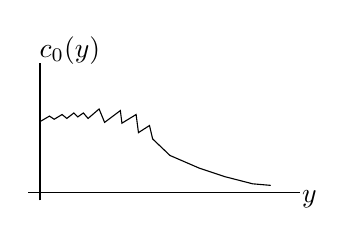
\begin{tikzpicture}[x=1cm,y=1cm]
\draw (-0.15,0)--(3.3,0);
\draw (0,-0.1)--(0,1.65);
\node at (0.38,1.8) {$c_0(y)$};
\node at (3.42,-0.08) {$y$};
\draw (0,0.9)--(0.12,0.97)--(0.18,0.93)--(0.28,0.99)--(0.34,0.94)--(0.43,1.01)--(0.48,0.96)--(0.55,1.01)--(0.61,0.94)--(0.75,1.06)--(0.82,0.89)--(1.02,1.04)--(1.04,0.88)--(1.22,0.99)--(1.25,0.76)--(1.39,0.85)--(1.43,0.68)--(1.65,0.47)--(2.02,0.31)--(2.35,0.20)--(2.7,0.11)--(2.93,0.09);
\end{tikzpicture}
\end{adjustbox}
\end{center}
частота осцилляций задаётся $\rho$ --- нулём
\Unclear{GELFAND-P001341}{zero-map}{$\rho\mapsto\zeta(2\rho)$; возможное чтение первого знака: $s$ вместо $\rho$.}

[Над словами «частота осцилляций», стрелка к ним:]
при $y\to0$.

(см. повед. преобр. Меллина)

\SourceFigure{GELFAND-P001341}{horocycle-sketch}{Слева перед строкой о получении $c_0(y)$: полоса с двумя вертикальными сторонами, большая верхняя дуга с направлением вправо вниз, внутренние нисходящие кривые и несколько нижних горизонтальных линий. В нижней части пересечения и возможные стрелки наложены друг на друга; их точная конфигурация не восстановлена.}
$c_0(y)$ получ. интегрир. по
\Unclear{GELFAND-P001341}{horocycle-word}{пост. орициклам! (возможно: раст. орициклу!)}

Если
\begin{equation*}
c_0(y)\sim\sum a_\lambda y^\lambda,\quad
\text{то}\quad
\int_0^1 y^{\lambda+s-2}\,dy=\frac1{\lambda-1+s}
\quad\Rightarrow\quad
\text{возникает полюс при }s=1-\lambda.
\end{equation*}
Берем $\Phi$ --- хар. ф-ю обл. и потом её размножаем. Получится

[Обведённая вставка со стрелкой к «обл.»:]
с объемом $=\frac13$ полного

\begin{equation}
a_1+\sum a_\rho y^{3/4}
\cos\left(\frac\tau2\log y-\varphi\right)
\tag{47}
\end{equation}
[Под $y^{3/4}$ через две вертикальные черты: $y^{1-\rho/2}$.]
\Unclear{GELFAND-P001341}{eq47-power-note}{[Соотношение степеней в приписке под (47) сохранено как в источнике.]}
\Unclear{GELFAND-P001341}{eq47-cancelled}{[Справа от (47) зачёркнут математический фрагмент; видны знак, похожий на $\tau$, буква $y$ и степень, похожая на $1-\rho$.]}

Асимпт. пересечений определяется нулями $\zeta$-ф-и.

\Unclear{GELFAND-P001341}{cancelled-known}{[Зачёркнуто; возможное чтение: «Известно, что».]}

(48) \underline{Теорема}
Пусть $\Phi(z)$ --- $\Gamma$-инвар.,
$c_0(y)$ --- пост. член для $\Phi$
\begin{equation*}
\Rightarrow\quad\int_0^\infty c_0(y)y^{s-2}\,dy
\end{equation*}
полюса в $s=1,\rho/2$

функц. ур-е $s\mapsto1-s$

\underline{Вычеты:} при $s=1$ это $a_1$ в (47)

\SourcePage{GELFAND-P001342}{73}
% SourcePNG: images/GELFAND-P001342.png; sha256=6ff91e1210544da2d516fe220dfd84907b15a0d7553f66fb6bb16990d5783619; dimensions=2408x3448
% ReviewCrop: {"region":"1342-top","bbox":[30,30,2320,1000],"scale":3}
% ReviewCrop: {"region":"1342-eq52","bbox":[50,980,2300,1620],"scale":3}
% ReviewCrop: {"region":"1342-mid","bbox":[125,1630,2225,2510],"scale":3}
% ReviewCrop: {"region":"1342-bottom","bbox":[20,2420,2360,3440],"scale":3}
% ReviewCrop: {"region":"1342-operator54","bbox":[245,3060,640,3250],"scale":6}
% ReviewCrop: {"region":"1342-psi54","bbox":[855,3050,1060,3230],"scale":6}
% ReviewCrop: {"region":"1342-discriminant","bbox":[1150,1200,1525,1325],"scale":6}
% ReviewCrop: {"region":"1342-minus50","bbox":[720,510,890,605],"scale":8}
% ReviewCrop: {"region":"1342-zero54","bbox":[705,3250,1090,3375],"scale":8}
% ReviewCrop: {"region":"1342-v-int","bbox":[305,2540,985,2935],"scale":6}
% ReviewCrop: {"region":"1342-characterization","bbox":[1290,2535,2330,2670],"scale":6}
% ReviewCrop: {"region":"1342-side","bbox":[1100,2650,2320,3030],"scale":5}
% ReviewCrop: {"region":"1342-caption","bbox":[1310,3280,2230,3435],"scale":5}
% ReviewCrop: {"region":"1342-bottomtext","bbox":[1780,3165,2380,3310],"scale":6}
% ReviewCrop: {"region":"1342-finalleft","bbox":[195,3330,715,3440],"scale":6}
% ReviewCrop: {"region":"1342-graph","bbox":[1390,3180,1820,3310],"scale":6}
\begin{equation}
\frac3\pi\int_{\Gamma\backslash H}\Phi(z)\,dV
=\lim_{y\to0}c_0(y)=c_0(0)
\tag{49}
\end{equation}
Полезность: вместо интегрирования можно считать $c_0(0)$, что легко!

\underline{Приложение.} Пусть
\begin{equation}
\varphi(z)=y^kK_n(z,-\bar z),\quad k\ge4\ \text{чётно},\quad n\ge1
\tag{50}
\end{equation}
\begin{equation}
\int_{\Gamma\backslash H}\Phi(z)\,dV=c_0(0)
\qquad\text{вычисляется!}
\tag{51}
\end{equation}
\Unclear{GELFAND-P001342}{eq51-normalization}{[В (51) коэффициент перед интегралом отсутствует.]}
(но это было известно)

Более интересно:
\begin{equation}
\begin{aligned}
\int_{\Gamma\backslash H}\Phi(z)E(z,s)\,dV
&=\sum_{t\in Z}\int_{\Gamma\backslash H}
\left(\sum_{\substack{Q\\\operatorname{disc}(Q)=t^2-4n}}R_{Q,t}(z)\right)E(z,s)\,dV=\\
&=\sum_{t\in Z}(....)\zeta_{Q(\sqrt{t^2-4n})}(s)
\end{aligned}
\tag{52}
\end{equation}
[Под $(....)$, стрелка вверх:]
нек-ое выражение

\begin{equation*}
\forall\ \text{расшир. поля}\quad
\begin{matrix}K\\\vert\quad2\\Q\end{matrix}
\qquad
\zeta_K(s)=\sum\frac1{N(\,)^{s}}=\zeta(s)L(s)
\end{equation*}
\begin{equation*}
\zeta(\rho)=0\quad\Rightarrow\quad\zeta_K(\rho)=0
\end{equation*}
Получается, что
\begin{equation}
\int_{\Gamma\backslash H}\Phi(z)E(z,\rho)\,dV=0
\quad\text{при условии, что}\quad\zeta(\rho)=0!
\tag{53}
\end{equation}
[Под формулой зачёркнуто: $\zeta(\rho)=0$.]

Введём пр-во всех таких ф-й
\begin{equation*}
V=\{\varphi(z)\text{ на }\Gamma\backslash H\}
\end{equation*}
\begin{equation*}
\int_{\Gamma\backslash H}\psi(z)\varphi(z)=0
\end{equation*}
\Unclear{GELFAND-P001342}{cancelled-integral-domain}{[Под последним интегралом над $\Gamma\backslash H$ зачёркнут короткий неразборчивый предел.]}

[Справа, за двойной вертикальной чертой:]
Это характеризация корней $\rho$!!

(Спектр представления в $V$!)

(опер. Лапласа)

[Ниже и левее:]
Спектр опер. Лапл.

[Стрелка вниз:]
если оно унит., то получается гипотеза Римана.

[Слева, подчёркнуто, стрелка к (54):]
$\Phi$ образуют большой набор

(Отсутствие других нулей не доказано)

\Unclear{GELFAND-P001342}{eq54-operator}{[Петлеобразный знак оператора с индексом $D$ в (54) неуверенно прочитан как $\mathcal{L}_D$.]}
\begin{equation}
(\mathcal{L}_D\Psi)(z)
=\sum_{\substack{A,B,C\in Z\\B^2-4AC=0}}
\Psi\left(\frac{A|z|^2+Bx+C}{y}\right)
\tag{54}
\end{equation}
\Unclear{GELFAND-P001342}{eq54-discriminant}{[Условие под суммой в (54) прочитано буквально: $B^2-4AC=0$.]}
[Под $z$ в левой части стрелка вверх от $\Gamma\backslash H$.]

Автом. $\Gamma$-инвариантна

\begin{center}
\begin{adjustbox}{max width=\linewidth}
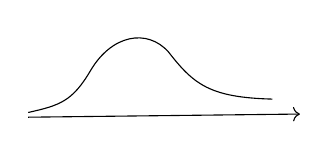
\begin{tikzpicture}[x=1cm,y=1cm]
\draw[->] (0,0)--(3.45,0.04);
\draw (0,0.06)..controls(0.40,0.15)and(0.56,0.20)..(0.79,0.59)
..controls(1.06,1.05)and(1.51,1.13)..(1.78,0.83)
..controls(2.10,0.42)and(2.30,0.25)..(3.10,0.23);
\end{tikzpicture}
\end{adjustbox}
\end{center}
$\Psi$ --- гладкая и убывающая

это --- опис. $W$;\qquad $V=W^\perp$

\SourcePage{GELFAND-P001343}{unlabelled}
% SourcePNG: images/GELFAND-P001343.png; sha256=3c9d3b6fc3f6a3ea17e449232c6851f7a781b968289964ce7f65f0fc5f92f375; dimensions=2408x3448
% ReviewCrop: {"region":"cross-1343-name","bbox":[290,1345,555,1467],"scale":8}
% ReviewCrop: {"region":"cross-1343-cancel","bbox":[1450,1365,1695,1473],"scale":8}
% ReviewCrop: {"region":"cross-1343-psi","bbox":[730,75,812,185],"scale":8}
% ReviewCrop: {"region":"top-formula","bbox":[80,45,1600,260],"scale":3}
% ReviewCrop: {"region":"top-operator","bbox":[525,60,875,230],"scale":6}
% ReviewCrop: {"region":"top-text","bbox":[210,265,1420,430],"scale":3}
% ReviewCrop: {"region":"laplacian","bbox":[325,413,1620,610],"scale":3}
% ReviewCrop: {"region":"heading","bbox":[150,1210,975,1350],"scale":3}
% ReviewCrop: {"region":"task-start","bbox":[150,1350,2220,1485],"scale":3}
% ReviewCrop: {"region":"task-continuation","bbox":[160,1470,2270,1680],"scale":3}
% ReviewCrop: {"region":"speaker","bbox":[145,1690,565,1830],"scale":3}
% ReviewCrop: {"region":"zeta-values","bbox":[40,1815,1990,2380],"scale":2}
% ReviewCrop: {"region":"negative-three","bbox":[1490,2200,1990,2380],"scale":6}
% ReviewCrop: {"region":"moduli","bbox":[50,2370,2250,2720],"scale":3}
% ReviewCrop: {"region":"eisenstein","bbox":[35,2750,2310,3350],"scale":2}
% ReviewCrop: {"region":"coefficient-cancellation","bbox":[195,3050,450,3210],"scale":6}
% ReviewCrop: {"region":"right-edge","bbox":[2363,117,2408,215],"scale":10}
% ReviewCrop: {"region":"task-name","bbox":[290,1345,555,1467],"scale":8}
% ReviewCrop: {"region":"task-cancelled","bbox":[1450,1365,1695,1473],"scale":8}
% ReviewCrop: {"region":"task-triangles","bbox":[755,1475,1030,1580],"scale":6}
% ReviewCrop: {"region":"top-psi","bbox":[740,81,805,189],"scale":10}
% ReviewCrop: {"region":"moduli-cancelled","bbox":[1530,2490,1690,2615],"scale":8}
% ReviewCrop: {"region":"speaker-spelling","bbox":[325,1698,510,1797],"scale":6}
\begin{equation}
\tag{55}
\int_{\Gamma\backslash H}E(z,s)\mathcal{L}_{D}\Psi(z)\,dV
=(*)\zeta_{\mathbb{Q}(\sqrt{D})}(s).
\end{equation}
\Unclear{GELFAND-P001343}{top-operator}{обозначение оператора: $\mathcal{L}_{D}$?}

меняя $D$, получаем $\zeta$-ф-ю Римана

Оператор надо взять стандартный:
\begin{equation*}
\Delta=y^2\left(\frac{\partial^2}{\partial x^2}+\frac{\partial^2}{\partial y^2}\right),
\qquad \Delta(W)\subset W
\end{equation*}

[У правого обреза: \Unclear{GELFAND-P001343}{right-edge}{неразборчивый фрагмент буквы}.]

\bigskip
16/II-87. \underline{Сем. Гельфанда.}

\underline{\underline{Зад.}} (\Unclear{GELFAND-P001343}{task-name}{Казаков?}).
Сколько триангуляций сферы
[зачёркнуто: \Unclear{GELFAND-P001343}{task-cancelled}{неразборчивое слово}]
с закраш. в 2 цвета (бел. и черн.) $\Delta$-ками с фиксир. числом чёрных и белых и
фикс. длине границ (между белым и чёрным).

\underline{\underline{Дон Цагир.}}

\begin{equation}
\tag{1}
\zeta(s)=\sum_{n=1}^{\infty}\frac{1}{n^s},\quad
\text{тогда }\zeta(2)=\frac{\pi^2}{6},\quad \zeta(4)=\frac{\pi^4}{90}
\end{equation}
\begin{equation*}
\zeta(2n)=\frac{(-1)^{n-1}2^{2n-1}B_{2n}}{(2n)!}\pi^{2n}
\end{equation*}
\begin{equation}
\tag{2}
\zeta(0)=-\frac12,\quad \zeta(-1)=-\frac1{12},\quad
\zeta(-2)=0,\quad \zeta(-3)=\frac1{252}
\end{equation}
\Unclear{GELFAND-P001343}{negative-three}{в источнике $\zeta(-3)=1/252$}

\begin{equation}
\tag{3}
\underset{\text{(Harer, Zagier)}}{\zeta(1-2g)=\chi(\mathcal{M}_g)}
\qquad (?)
\end{equation}
$\mathcal{M}_g$ — пр-во модулей
[зачёркнуто: \Unclear{GELFAND-P001343}{moduli-cancelled}{неразборчивое слово}]
пов. рода $g$

$\chi(\mathcal{M}_g)$ — его эйлерова хар-ка.

\Unclear{GELFAND-P001343}{moduli-identity}{равенство (3) с авторским знаком вопроса}

$k=4,6,8,10,\ldots$
\begin{equation}
\tag{4}
E_k(z)=\frac12\sum_{(c,d)=1}\frac{1}{(cz+d)^k}
\end{equation}
\begin{equation}
\tag{5}
\begin{aligned}
\zeta(k)E_k(z)&=\sum_{(m,n)\ne(0,0)}\frac{1}{(mz+n)^k}\\
&=\zeta(+k)+\frac{(2\pi i)^k}{(k-1)!}\sum_{n=1}^{\infty}\sigma_{k-1}(n)q^n,
\end{aligned}
\end{equation}
[В первом $\zeta(k)$ перед $k$ зачёркнуто:
\Unclear{GELFAND-P001343}{coefficient-cancellation}{неразборчивый знак}.]
\Unclear{GELFAND-P001343}{eisenstein-normalization}{в (5) перед суммой по $(m,n)$ множитель не записан}

\SourcePage{GELFAND-P001344}{74}
% SourcePNG: images/GELFAND-P001344.png; sha256=4104cd9ca33eaef3018ac1a86a6eee96d99a79ec53730ed3b718d14c783bcdaf; dimensions=2408x3448
% ReviewCrop: {"region":"cross-1344-coefficient","bbox":[1055,478,1255,550],"scale":8}
% ReviewCrop: {"region":"cross-1344-pi","bbox":[917,440,1008,506],"scale":10}
% ReviewCrop: {"region":"sigma-definition","bbox":[10,75,1340,280],"scale":3}
% ReviewCrop: {"region":"eisenstein-examples","bbox":[130,285,1925,690],"scale":3}
% ReviewCrop: {"region":"e4-coefficient","bbox":[990,295,1290,432],"scale":6}
% ReviewCrop: {"region":"e8-coefficient","bbox":[855,435,1460,585],"scale":6}
% ReviewCrop: {"region":"modular-relations","bbox":[205,683,1920,1086],"scale":3}
% ReviewCrop: {"region":"cancelled-left","bbox":[393,789,560,950],"scale":6}
% ReviewCrop: {"region":"all-even","bbox":[45,1090,1585,1430],"scale":3}
% ReviewCrop: {"region":"hecke-title","bbox":[110,1575,839,1805],"scale":3}
% ReviewCrop: {"region":"cusp","bbox":[211,1810,1695,2180],"scale":3}
% ReviewCrop: {"region":"gamma-derivation","bbox":[204,2180,1810,2828],"scale":2}
% ReviewCrop: {"region":"numerator-cancellation","bbox":[594,2600,768,2707],"scale":8}
% ReviewCrop: {"region":"mellin-formula","bbox":[50,2835,2320,3155],"scale":3}
% ReviewCrop: {"region":"transformation","bbox":[173,3142,1830,3447],"scale":3}
% ReviewCrop: {"region":"e8-arrow","bbox":[322,548,396,613],"scale":10}
% ReviewCrop: {"region":"e8-exponent","bbox":[917,440,1008,506],"scale":10}
% ReviewCrop: {"region":"parabolic-word","bbox":[808,1987,1237,2101],"scale":6}
% ReviewCrop: {"region":"product-e10","bbox":[300,1423,1110,1546],"scale":3}
где $\sigma_{k-1}(n)=\sum_{d\mid n}d^{k-1}$, $q=e^{2\pi iz}$

\begin{equation*}
M_4\ni E_4\zeta(4)=\zeta(4)+\frac{8\pi^4}{3}(q+28q^2+\ldots)
\qquad \text{(вес 4)}
\end{equation*}
\Unclear{GELFAND-P001344}{e4-coefficient}{в источнике $28q^2$}

\begin{equation*}
\underset{\substack{\Uparrow\\M_8}}{E_8}(z)\zeta(8)
=\zeta(8)+\underline{\ldots\pi^8}(q+129q^2+\ldots)
\qquad \text{(вес 8)}
\end{equation*}
\Unclear{GELFAND-P001344}{e8-exponent}{показатель при $\pi$: 8 или 2}
\Unclear{GELFAND-P001344}{e8-coefficient-bar}{под $\ldots\pi^8$ горизонтальная черта; под чертой ничего не записано}

\begin{equation*}
\dim M_8=1;\qquad \dim M_4=1
\end{equation*}
[Зачёркнуто: \Unclear{GELFAND-P001344}{cancelled-left}{неразборчивое обозначение}.]
\begin{equation*}
\Rightarrow E_4^2=cE_8\qquad \text{(веса совпадают)}
\end{equation*}
\begin{equation*}
\zeta(4)=\pi^4/90\quad\Rightarrow\quad\zeta(8)=\pi^8/9450
\end{equation*}

Таким образом:

По $\underset{\substack{\Vert\\\frac{\pi^4}{90}}}{\zeta(4)}$
и $\underset{\substack{\Vert\\\pi^6/945}}{\zeta(6)}$
находятся все $\zeta(2n)$

\begin{equation*}
E_4E_6=cE_{10}\quad\text{и т.д.}
\end{equation*}

$L$-ряды Гекке

Пусть
\begin{equation*}
f(z)\in M_k(SL_2(\mathbb{Z}))
\end{equation*}
\begin{equation*}
f(z)=\sum_{n=0}^{\infty}a_nq^n\qquad \text{модул. форма веса }k
\end{equation*}
\begin{equation*}
a_0=0\Rightarrow f\in S_k\qquad
\begin{gathered}\text{(параболические)}\\\text{cusp form}\end{gathered}
\end{equation*}
\begin{equation*}
L(f,s):=\sum_{n=1}^{\infty}\frac{a_n}{n^s}
\end{equation*}
\begin{equation*}
\Gamma(s)=\lambda^s\int_0^{\infty}y^{s-1}e^{-\lambda y}\,dy
\end{equation*}
\begin{equation*}
\Gamma(s)\sum_{n=1}^{\infty}\frac{a_n}{(2\pi n)^s}
=\int_0^{\infty}y^{s-1}\left(\sum_{n=1}^{\infty}a_ne^{-2\pi ny}\right)dy
\end{equation*}
[В числителе после $a_n$ зачёркнуто:
\Unclear{GELFAND-P001344}{numerator-cancellation}{неразборчивые знаки}.]

\begin{equation}
\tag{6}
\Gamma(s)(2\pi)^{-s}L(f,s)=\int_0^{\infty}y^{s-1}f(iy)\,dy
\end{equation}
\begin{equation*}
\begin{gathered}\text{(если }f\text{ параболическая)}\\f\in S_k\end{gathered}
\end{equation*}
Интеграл справа всегда сходится.

\begin{equation*}
f\left(-\frac1z\right)=z^kf(z),\qquad
f\left(\frac{i}{y}\right)=(-1)^{k/2}y^kf(iy)
\end{equation*}
Отсюда

\SourcePage{GELFAND-P001345}{unlabelled}
% SourcePNG: images/GELFAND-P001345.png; sha256=cf12ba9e59734347d1cf593ece966a89d95c0f11193e63e1756326c7500cf9c9; dimensions=2408x3448
% ReviewCrop: {"region":"cross-1345-decimals","bbox":[315,2360,1340,2600],"scale":5}
% ReviewCrop: {"region":"cross-1345-range","bbox":[1350,2830,1940,2970],"scale":6}
% ReviewCrop: {"region":"cross-1345-cancellations","bbox":[810,848,970,1110],"scale":6}
% ReviewCrop: {"region":"cross-1345-eisenstein","bbox":[260,2668,1250,2850],"scale":5}
% ReviewCrop: {"region":"top-notation","bbox":[265,10,1470,515],"scale":3}
% ReviewCrop: {"region":"theorem-cancellations","bbox":[755,830,1110,1105],"scale":5}
% ReviewCrop: {"region":"theorem-prose","bbox":[230,1120,2270,1355],"scale":3}
% ReviewCrop: {"region":"period-table","bbox":[120,1880,2200,2380],"scale":3}
% ReviewCrop: {"region":"period-constants","bbox":[310,2370,1320,2635],"scale":4}
% ReviewCrop: {"region":"eisenstein-cancellation","bbox":[265,2640,1260,3000],"scale":4}
% ReviewCrop: {"region":"bottom-formula","bbox":[100,2930,2340,3385],"scale":3}
% ReviewCrop: {"region":"table-note","bbox":[1060,2230,1650,2380],"scale":5}
% ReviewCrop: {"region":"cancel-rational-first","bbox":[810,893,928,984],"scale":10}
% ReviewCrop: {"region":"cancel-rational-second","bbox":[810,1005,950,1090],"scale":10}
% ReviewCrop: {"region":"eisenstein-erasure","bbox":[830,2650,983,2820],"scale":8}
% ReviewCrop: {"region":"eq11-limits","bbox":[1360,2810,2010,2950],"scale":4}
% ReviewCrop: {"region":"scalar-note","bbox":[1080,3060,2340,3270],"scale":3}
% ReviewCrop: {"region":"prose-insert","bbox":[230,1100,2270,1350],"scale":3}
\begin{equation*}
(7)\qquad \Gamma(s)(2\pi)^{-s}L(f,s)=(-1)^{k/2}\,(s\to k-s)
\end{equation*}
[Выражение $\Gamma(s)(2\pi)^{-s}L(f,s)$ охвачено снизу скобкой; от неё вниз к $L^*(f,s)$ в (8) проведены две вертикальные черты. Рядом:] (функц. ур-е)
\begin{equation*}
(8)\qquad L^*(f,s)=(-1)^{k/2}L^*(f,k-s)
\end{equation*}

(9)\qquad \underline{Теор.} (Eichler + Shimura + Manin)

Если $f(z)\in S_k(SL_2 Z)$ форма Гекке, то $\exists\,\omega_+,\omega_-\in R$ (зав. только от $f$), такие что
\begin{align*}
L^*(f,n)&=(\text{алг. число})\,\omega_-,\qquad n=2,4,\ldots,k-2,\\
L^*(f,n)&=(\text{алг. число})\,\omega_+,\qquad n=1,3,\ldots,k-1.
\end{align*}
[В первой строке перед «число» зачёркнуто: \Unclear{GELFAND-P001345}{even-cancel}{рац.?}; сверху надписано «алг.». Во второй строке перед «число» зачёркнуто: \Unclear{GELFAND-P001345}{odd-cancel}{рац.?}; сверху надписано «алг.».]

$\omega_-,\omega_+$, вероятно, трансцендентны; это док. не для $SL_2(Z)$, а для других групп (с комплексным \underline{умножением})

\begin{equation*}
(10)\qquad r_n(f)=\int_0^\infty f(iy)y^n\,dy,\qquad n=0,1,\ldots,k-2.
\end{equation*}
[Под $r_n(f)$ черта вниз к слову:] период

\underline{Пример.}
\begin{align*}
\Delta(z)\in S_{12}(SL_2(Z))&=q-24q^2+252q^3+\ldots=\\
&=q\prod_1^\infty(1-q^n)^{24}
\end{align*}
\begin{equation*}
\begin{array}{c|cccccc}
 &10&9&8&7&6&\\
n&0&1&2&3&4&5\\
r_n(\Delta)&\frac{192}{691}\omega_+&\frac{384}{5}\omega_-&\frac{16}{135}\omega_+&40\omega_-&\frac{8}{105}\omega_+&32\omega_-
\end{array}
\qquad r_n=r_{10-n}
\end{equation*}
[Под $32\omega_-$ скобка с подписью:] опр. $\omega_-$

(только отнош. сущ.)
\begin{align*}
\omega_+&=0.021446067\ldots\\
\omega_-&=0.0000482774800\ldots
\end{align*}

\begin{equation*}
(10')\qquad G_k(z)=\underbrace{-\frac{B_k}{2k}}_{\zeta(1-k)}\,E_k(z)\qquad(\text{ряд Эйзеншт.})
\end{equation*}
[Начальная буква в $G_k(z)$ исправлена или обведена: \Unclear{GELFAND-P001345}{eisenstein-initial}{предыдущее начертание $E$?}. Между $-B_k/(2k)$ и $E_k(z)$ зачёркнуто: \Unclear{GELFAND-P001345}{eisenstein-erasure}{неразборчивый множитель; начало $2$?}.]
\Unclear{GELFAND-P001345}{eisenstein-normalization}{под $-B_k/(2k)$ написано $\zeta(1-k)$}

[Справа над (11):]
\begin{equation*}
\frac{k}{2}<n\le k-2
\end{equation*}
\Unclear{GELFAND-P001345}{eq11-range}{$k/2<n\le k-2$}
\begin{equation*}
(11)\qquad -\frac{4n}{B_{2n}}\left(
\underset{\substack{\uparrow\\S_k}}{f},\,
\underset{\substack{\uparrow\\M_{2n}}}{G_{2n}}
\underset{\substack{\uparrow\\M_{k-2n}}}{G_{k-2n}}
\right)
\end{equation*}
а (одна из них параболич. $\Rightarrow$ ск. пр. сход.)
[От «из них» стрелка вниз влево к подынтегральному произведению.]
\begin{equation*}
\left(\text{скал. произв.:}\qquad(f,g)=\int_{\Gamma\backslash H}f(z)\overline{g(z)}y^k\,\frac{dx\,dy}{y^2}\right)
\end{equation*}

\SourcePage{GELFAND-P001346}{75}
% SourcePNG: images/GELFAND-P001346.png; sha256=74ee82e8d18b76b7f511d27717caaeef8f52cc06163d43eceffabed1cc00f6c8; dimensions=2408x3448
% ReviewCrop: {"region":"top-formula","bbox":[80,20,1755,430],"scale":3}
% ReviewCrop: {"region":"gamma-fraction","bbox":[1200,530,2380,780],"scale":3}
% ReviewCrop: {"region":"imaginary-part","bbox":[365,733,1390,930],"scale":4}
% ReviewCrop: {"region":"insertion-prose","bbox":[300,920,2140,1090],"scale":3}
% ReviewCrop: {"region":"integral-transform","bbox":[300,1080,1670,1550],"scale":3}
% ReviewCrop: {"region":"fourier-unfolding","bbox":[320,1560,2370,2235],"scale":3}
% ReviewCrop: {"region":"conclusion","bbox":[250,2250,1610,3120],"scale":3}
% ReviewCrop: {"region":"factorial","bbox":[905,2810,1130,2980],"scale":8}
% ReviewCrop: {"region":"mobius-signs","bbox":[866,748,1070,880],"scale":8}
% ReviewCrop: {"region":"insertion-letter","bbox":[937,930,1151,1045],"scale":8}
% ReviewCrop: {"region":"fourier-conjugate","bbox":[1260,1860,1720,2070],"scale":5}
% ReviewCrop: {"region":"conclusion-factor","bbox":[260,2770,900,3015],"scale":4}
\begin{equation*}
(12)\qquad(11)=\int_{\Gamma\backslash H}f(z)
\sum_{\left(\begin{smallmatrix}\cdot&\cdot\\c&d\end{smallmatrix}\right)\in
\left(\begin{smallmatrix}1&*\\0&1\end{smallmatrix}\right)\backslash SL_2(Z)}
\frac{1}{(c\bar z+d)^{2n}}\,\overline{G_{k-2n}(z)}\,y^k\,dV
\end{equation*}
[Под $\overline{G_{k-2n}(z)}$ скобка; к ней направлена двойная стрелка снизу от дроби:]
\begin{equation*}
\frac{G_{k-2n}(\gamma z)}{(c\bar z+d)^{k-2n}}
\qquad\left(\text{т.к. }G(\gamma z)=(cz+d)^{k-2n}G(z)\right)
\end{equation*}
\Unclear{GELFAND-P001346}{upper-transform-conjugation}{числитель дроби $G_{k-2n}(\gamma z)$ без черты}

\begin{equation*}
\operatorname{Im}(\gamma z)=\operatorname{Im}\left(\frac{az-ib}{cz-id}\right)=\frac{y}{|cz+d|^2}
\end{equation*}
\Unclear{GELFAND-P001346}{mobius-signs}{$(az-ib)/(cz-id)$; возможное чтение знаков как раздельно написанных плюсов}

И можно вставить $\gamma$ \Unclear{GELFAND-P001346}{insertion-letter}{в?; у?} $f$: $f(\gamma z)$, заменив множитель

Получим:
\begin{align*}
&\sum_\gamma\int_{\mathcal F}f(\gamma z)\overline{G_{k-2n}(\gamma z)}\operatorname{Im}(\gamma z)^k\,dV=\\
&=\sum_\gamma\int_{\gamma\mathcal F}f(z)\overline{G_{k-2n}(z)}(\operatorname{Im}z)^k\,dV=\\
&=\int_{z\to z+1\backslash H}f(z)G_{k-2n}(z)y^k\frac{dx\,dy}{y^2}
=\sum_{n=1}^\infty a(n)\overline{b(n)}\int_0^\infty e^{-4\pi ny}y^{k-2}\,dy
\end{align*}
[Область интегрирования $z\to z+1\backslash H$ охвачена снизу скобкой; под ней две черты к:]
\begin{equation*}
\int_0^\infty\int_0^1
\end{equation*}
[От $f(z)$ две вертикальные черты к:]
\begin{equation*}
\sum_{n=1}^\infty a(n)e^{2\pi inz}
\end{equation*}
[От $G_{k-2n}(z)$ две наклонные черты вниз вправо к:]
\begin{equation*}
\sum_{m=0}^\infty b(m)e^{-2\pi im\bar z}
\end{equation*}
\Unclear{GELFAND-P001346}{unfolding-conjugation}{в третьем интеграле $G_{k-2n}(z)$ без черты; в нижнем ряде $b(m)$ без черты}

Итог:
\begin{align*}
f(z)&=\sum_{n=1}^\infty a(n)q^n\in S_k,\\
G(z)&=\sum_{m=0}^\infty b(m)q^m\in M_{k-2n},\qquad n\ge2
\end{align*}
\begin{equation*}
(13)\qquad-\frac{4n}{B_{2n}}\left(f,\underset{k-2n}{G}\cdot\underset{2n}{G_{2n}}\right)
=\frac{(k-1)!}{(4\pi)^{k-1}}\sum_{m=1}^\infty\frac{a(m)b(m)}{m^{k-1}}
\end{equation*}
(свёртка)

\Unclear{GELFAND-P001346}{bottom-factorial}{в числителе $(k-1)!$}
\Unclear{GELFAND-P001346}{bottom-coefficient}{в (13) $a(m)b(m)$ без черты над $b(m)$}

\SourcePage{GELFAND-P001347}{unlabelled}
\begin{equation*}
G=G_{k-2n}(z)=(*)+\sum_{m=1}^{\infty}\sigma_{k-1-2n}(m)q^m.
\end{equation*}
\begin{equation*}
f=\sum_{m=1}^{\infty}a(m)q^m=\text{форма Гекке}.
\end{equation*}
[Зачёркнуто: $=\prod_p[1+\frac{a(p)}{p^s}+$]
\begin{equation*}
\left(\begin{gathered}
a(mm')=a(m)a(m')\quad\text{при }(m,m')=1,\\
a(2^a3^b5^c\ldots)=a(2^a)a(3^b)\ldots
\end{gathered}\right.
\end{equation*}
Тогда
\begin{equation*}
\tag{14}\sum\frac{a(m)}{m^s}
=\prod_p\left[1+\frac{a(p)}{p^s}+\frac{a(p^2)}{p^{2s}}+\ldots\right].
\end{equation*}
\begin{equation*}
a(m)a(n)=\sum_{d\mid m,n}d^{k-1}a\left(\frac{mn}{d^2}\right),
\qquad b(p)=1+p^{k-1-2n}.
\end{equation*}
$\Rightarrow$ ряд вычисляется
\begin{equation*}
\underbrace{\frac{(k-2)!}{(4\pi)^{k-1}}
\sum_{m=1}^{\infty}\frac{a(m)\sigma_{k-1-2n}(m)}{m^{k-1}}}
_{\displaystyle\Vert\quad L(f,k-1)L(f,2n)/\zeta(2n)}
=\underbrace{-\frac{4n}{B_{2n}}(f,\overbrace{G_{k-2n}\cdot G_{2n}})}
_{\displaystyle\Vert\quad\alpha\cdot(f,f)}.
\end{equation*}
[К скобке над $G_{k-2n}\cdot G_{2n}$:]
$\alpha f+\beta f_1+\ldots$, $f_j$ --- базис.
[Под $\alpha\cdot(f,f)$ зачёркнутый знак:]
\Unclear{GELFAND-P001347}{pairing-overwrite}{нечитаемый знак}.
$\Downarrow\quad\alpha\in\overline{\mathbb Q}^{*}$ (алгебрич.)

Все коэфф. ряда Эйзеншт. --- рац. числа.

Итак
\begin{equation*}
L(f,2n)/\zeta(2n)\quad\text{не зав. от }n
\quad\Rightarrow\quad\text{теорема }
\text{\ReaderApparatusRef{1}{1}}\text{ Делиня }D.
\end{equation*}
(Rankin, 1953)
\begin{equation*}
S_{2k}\quad\text{\ReaderApparatusRef{2}{1}}
\quad S_{2k}^{\mathbb Q}=\{f=\sum a(n)q^n;\ a(n)\in\mathbb Q\}.
\end{equation*}
[Под левым $S_{2k}$:]
\Unclear{GELFAND-P001347}{rational-left-margin}{$\eta^2$ / $\text{?}^{2}$}.
\begin{center}
\ReaderDiagramPair{figures/gelfand-0146-d01-gelfand-p001347-original.png}{GELFAND-P001347}{%
\begin{adjustbox}{max width=\linewidth}
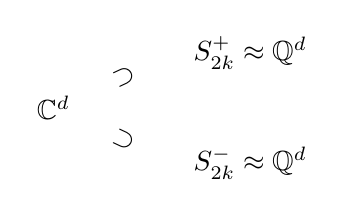
\begin{tikzpicture}
\node at (0,0) {$\mathbb C^d$};
\node at (2.5,.7) {$S_{2k}^{+}\approx\mathbb Q^d$};
\node at (2.5,-.7) {$S_{2k}^{-}\approx\mathbb Q^d$};
\node[rotate=25] at (.9,.4) {$\supset$};
\node[rotate=-25] at (.9,-.4) {$\supset$};
\end{tikzpicture}
\end{adjustbox}
}

\end{center}
(хотя, 3 разные рац. структуры в $S_{2k}$)
\begin{equation*}
S_{2k}^{\pm,\mathbb Q}\otimes\mathbb C=S_{2k}.
\end{equation*}


\ReaderNotesStart{GELFAND-P001347}
\ReaderNote{1}{\Unclear{GELFAND-P001347}{name-prefix}{(?) / (о)}}
\ReaderNote{2}{\Unclear{GELFAND-P001347}{rational-separator}{перечёркнутый или подчёркнутый знак}}
\ReaderNotesEnd
\SourcePage{GELFAND-P001348}{76}
\begin{equation*}
S_{2k}^{+}:=\{f\in S_{2k}\mid\tau_n(f)\in\mathbb Q,\ n=0,2,4,\ldots,k-2\}.
\end{equation*}
\begin{equation*}
S_{2k}^{-}:=\{\text{---||---}\quad n=1,3,5,\ldots\}.
\end{equation*}
\begin{equation*}
k=12,\qquad\dim S_{12}=1.
\end{equation*}
\begin{equation*}
S_{12}^{+}=\{f\mid\tau_0(f),\tau_2(f),\tau_4,\tau_6,\tau_8,\tau_{10}\in\mathbb Q\}.
\end{equation*}
Не очевидно, что размерность сохр!

\underline{Лит-ра}: статья \underline{Kohnen} $+$ \underline{Zagier}

Modular forms with rational coefficients

(conf. Ed. \underline{Rankin} --- книга)

\SourcePage{GELFAND-P001349}{unlabelled}
\underline{2/III--87 г.}\qquad \underline{В. Казаков.}
\underline{Задача о склейках пов. рода $g$ из $2n$-угольника.}

\begin{center}
\ReaderDiagramPair{figures/gelfand-0146-d02-gelfand-p001349-original.png}{GELFAND-P001349}{%
\begin{adjustbox}{max width=\linewidth}
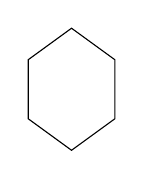
\begin{tikzpicture}[x=1cm,y=1cm]
\draw (0,0.6)--(0.55,1)--(1.1,0.6)--(1.1,-0.15)--(0.55,-0.55)--(0,-0.15)--cycle;
\end{tikzpicture}
\end{adjustbox}
}

\end{center}
$2n$-угольник; склеив \Unclear{GELFAND-P001349}{header-hook}{галочка / $\gamma$}
\Unclear{GELFAND-P001349}{opposite-word}{противоп. / противопол.} ориент. стороны (попарно).

$g$ --- род возникш. мн-зия.
Сколько различных способов, при к-рых получ. пов. рода $g$?
$f_n^g$ --- число таких способов склейки.

(Можно Запретить некоторые склейки.
\underline{Запреты:} 1)
\begin{center}
\ReaderDiagramPair{figures/gelfand-0146-d03-gelfand-p001349-original.png}{GELFAND-P001349}{%
\begin{adjustbox}{max width=\linewidth}
\begin{tikzpicture}[x=1cm,y=1cm]
\node at (-0.5,0) {а)};
\draw (0,0)--(0.75,0.5); \draw (0,0)--(0.55,-0.7);
\fill (0,0) circle (0.035);
\draw[<->] (0.37,0.2) to[bend left=18] (0.37,-0.38);
\node at (1.7,0) {б)};
\draw (2.3,0.15)--(2.8,0.5)--(3.2,0.15);
\draw (2.8,0.5) circle (0.04);
\draw (2.7,-1)--(3.2,-1.05)--(3.45,-0.35);
\draw (3.2,-1.05) circle (0.04);
\draw[<->] (2.45,0.05) to[bend left=15] (2.85,-0.85);
\draw[<->] (3.02,0.1) to[bend right=8] (3.25,-0.65);
\end{tikzpicture}
\end{adjustbox}
}

\end{center}
2) [Зачёркнуто: ИЛИ] Запрещ. только б)\qquad 3) Запр. только а)

Всё сводится к случаю без запретов.)

\SourcePage{GELFAND-P001350}{85}
Произв. ф-я:
\begin{equation*}
(1)\quad f_n(N)=\text{\ReaderApparatusRef{1}{1}}\sum_{g=0}^{\infty}N^{-2g}f_n^g.
\end{equation*}
Тогда
\begin{equation*}
(2)\quad f_n(N)=(2\pi)^{-N^2/2}\int d^{N^2}\varphi\,\frac{\operatorname{tr}}{N}(\varphi^{2n})e^{-N\operatorname{tr}\varphi^2/2}
=\left\langle\frac{\operatorname{tr}}{N}\varphi^{2n}\right\rangle,
\end{equation*}
где $\varphi^+=\varphi$ --- эрмитова матрица $N\times N$.
\begin{center}
\ReaderDiagramPair{figures/gelfand-0146-d04-gelfand-p001350-original.png}{GELFAND-P001350}{%
\begin{adjustbox}{max width=\linewidth}
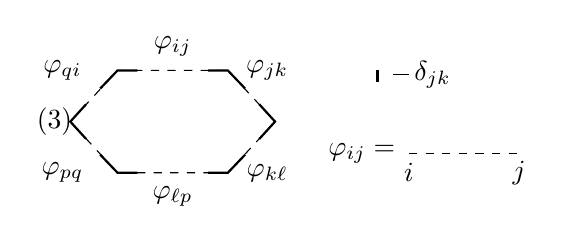
\begin{tikzpicture}[x=1cm,y=1cm]
\node at (-1.5,0) {(3)};
\draw[dashed] (-0.7,0.65)--(0.7,0.65)--(1.3,0)--(0.7,-0.65)--(-0.7,-0.65)--(-1.3,0)--cycle;
\draw[thick] (-0.92,0.42)--(-0.7,0.65)--(-0.45,0.65);
\draw[thick] (0.45,0.65)--(0.7,0.65)--(0.92,0.42);
\draw[thick] (1.1,0.22)--(1.3,0)--(1.1,-0.22);
\draw[thick] (0.92,-0.42)--(0.7,-0.65)--(0.45,-0.65);
\draw[thick] (-0.45,-0.65)--(-0.7,-0.65)--(-0.92,-0.42);
\draw[thick] (-1.1,-0.22)--(-1.3,0)--(-1.1,0.22);
\node at (0,0.95) {$\varphi_{ij}$}; \node at (1.2,0.65) {$\varphi_{jk}$};
\node at (1.2,-0.65) {$\varphi_{k\ell}$}; \node at (0,-0.95) {$\varphi_{\ell p}$};
\node at (-1.4,-0.65) {$\varphi_{pq}$}; \node at (-1.4,0.65) {$\varphi_{qi}$};
\draw[thick] (2.6,0.5)--(2.6,0.65);
\draw (2.8,0.6)--(3.0,0.6); \node at (3.3,0.6) {$\delta_{jk}$};
\node at (2.4,-0.4) {$\varphi_{ij}=$}; \draw[dashed] (3,-0.4)--(4.4,-0.4);
\node at (3,-0.65) {$i$}; \node at (4.4,-0.65) {$j$};
\end{tikzpicture}
\end{adjustbox}
}

\end{center}
Легко проверить, что
\begin{equation*}
(4)\quad \langle\varphi_{ij}\varphi_{k\ell}\rangle=\frac1N\delta_{i\ell}\delta_{jk},
\end{equation*}
или
\begin{center}
\ReaderDiagramPair{figures/gelfand-0146-d05-gelfand-p001350-original.png}{GELFAND-P001350}{%
\begin{adjustbox}{max width=\linewidth}
\begin{tikzpicture}[x=1cm,y=1cm]
\node at (-0.7,0) {$(4')$};
\draw (0.15,0.6)--(0,0.3)--(0.15,0); \draw (2.65,0.6)--(2.8,0.3)--(2.65,0);
\draw[dashed] (0.4,0.6)--(2.4,0.6); \draw[dashed] (0.4,0)--(2.4,0);
\node at (0.25,0.85) {$i$}; \node at (2.45,0.85) {$j$};
\node at (0.25,-0.25) {$\ell$}; \node at (2.45,-0.25) {$k$};
\node at (3.2,0.3) {$=$}; \draw[thick] (3.7,0.6)--(3.7,0); \draw[thick] (4.4,0.6)--(4.4,0);
\node at (3.7,0.85) {$i$}; \node at (3.7,-0.25) {$\ell$}; \node at (4.4,0.85) {$j$}; \node at (4.4,-0.25) {$k$};
\node at (6,0.8) {\underline{Обозначение:}};
\draw[thick] (5.7,0.35)--(5.6,-0.2); \node at (5.85,0.45) {$i$}; \node at (5.8,-0.3) {$k$}; \node at (6.5,0) {$=\delta_{ik}$};
\end{tikzpicture}
\end{adjustbox}
}

\end{center}
\begin{center}
\ReaderDiagramPair{figures/gelfand-0146-d06-gelfand-p001350-original.png}{GELFAND-P001350}{%
\begin{adjustbox}{max width=\linewidth}
\begin{tikzpicture}[x=1cm,y=1cm]
\node at (-2.6,0) {(5)};
\draw[dashed] (-0.6,0.7)--(0.6,0.7)--(1.2,0)--(0.6,-0.7)--(-0.6,-0.7)--(-1.2,0)--cycle;
\node at (-0.65,0.95) {$i_3$}; \node at (-1.5,0) {$i_2$};
\node at (-0.65,-1) {$i_1$}; \node at (0.65,-1) {$i_{2n}$};
\end{tikzpicture}
\end{adjustbox}
}

\end{center}
(6) \underline{Теор. Вика:} Пусть есть $2n$ гауссовых величин $\xi_1,\xi_2,\ldots,\xi_{2n}$. Тогда
([Зачёркнутая запись: \Incomplete{GELFAND-P001350}{wick-word}{короткая зачёркнутая запись под густыми штрихами; точное чтение не установлено}] [Вставлено сверху: линейные] ф-ии от $\varphi_{ik}$)
\begin{equation*}
\langle\xi_1\xi_2\cdots\xi_{2n}\rangle
=\sum_{P(i_1,\ldots,i_{2n})}\langle\xi_{i_1}\xi_{i_2}\rangle\langle\xi_{i_3}\xi_{i_4}\rangle\cdots.
\end{equation*}
[Под суммой зачёркнуто: \Incomplete{GELFAND-P001350}{cancel-index-first}{короткая прежняя строка индексов; начальный индекс похож на $i_2$, чтение не установлено}.]
Перестановки [зачёркнуто: $i_1,i_2,\ldots,i_{2n}$] $1,2,\ldots,2n$.
Сумма по всем разб. на пары.
\begin{center}
\ReaderDiagramPair{figures/gelfand-0146-d07-gelfand-p001350-original.png}{GELFAND-P001350}{%
\begin{adjustbox}{max width=\linewidth}
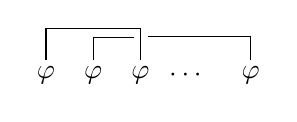
\begin{tikzpicture}[x=1cm,y=1cm]
\node at (0,0) {$\varphi$}; \node at (0.6,0) {$\varphi$}; \node at (1.2,0) {$\varphi$}; \node at (2.6,0) {$\varphi$};
\node at (1.8,0) {$\cdots$};
\draw (0,0.2)--(0,0.6)--(1.2,0.6)--(1.2,0.2);
\draw (0.6,0.2)--(0.6,0.48)--(1.12,0.48);
\draw (1.3,0.5)--(2.6,0.5)--(2.6,0.2);
\end{tikzpicture}
\end{adjustbox}
}

\end{center}
(\underline{Упражнение}: \Unclear{GELFAND-P001350}{exercise-word}{доказать? / оказать? / докажите? / окажите?})

Более общая теорема: пусть $\xi$ --- гаусс. величина, тогда
\begin{equation*}
(7)\quad \langle\xi f(\xi)\rangle=\langle\xi\xi\rangle\left\langle\frac{\partial f}{\partial\xi}\right\rangle.
\end{equation*}
\begin{equation*}
(8)\quad \langle\xi_i f(\xi)\rangle=\sum_j\langle\xi_i\xi_j\rangle\left\langle\frac{\partial f}{\partial\xi_j}\right\rangle.
\end{equation*}


\ReaderNotesStart{GELFAND-P001350}
\ReaderNote{1}{\Unclear{GELFAND-P001350}{sum-prefix}{зачёркнутый одиночный знак}}
\ReaderNotesEnd
\SourcePage{GELFAND-P001351}{unlabelled}
С пом. (7), (8) легко док. \underline{теор. Вика}
(\Unclear{GELFAND-P001351}{induction-word}{воспользовавш.? по $\xi$-числу?}).
\begin{center}
\ReaderDiagramPair{figures/gelfand-0146-d08-gelfand-p001351-original.png}{GELFAND-P001351}{%
\begin{adjustbox}{max width=\linewidth}
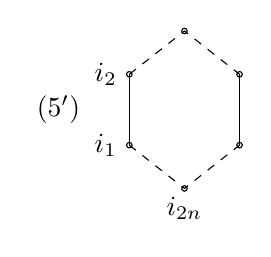
\begin{tikzpicture}[x=1cm,y=1cm]
\node at (-1.6,0) {$(5')$};
\draw[dashed] (-0.7,0.45)--(0,1)--(0.7,0.45);
\draw[dashed] (-0.7,-0.45)--(0,-1)--(0.7,-0.45);
\draw (-0.7,0.45)--(-0.7,-0.45); \draw (0.7,0.45)--(0.7,-0.45);
\draw (0,1) circle (0.035); \draw (0,-1) circle (0.035);
\draw (-0.7,0.45) circle (0.035); \draw (-0.7,-0.45) circle (0.035);
\draw (0.7,0.45) circle (0.035); \draw (0.7,-0.45) circle (0.035);
\node at (-1,0.45) {$i_2$}; \node at (-1,-0.45) {$i_1$}; \node at (0,-1.25) {$i_{2n}$};
\end{tikzpicture}
\end{adjustbox}
}

\end{center}
Интеграл (2) вычислим с пом. теор. Вика. Ясно, что
\begin{equation*}
(9)\quad \langle\operatorname{tr}\varphi^{2n}\rangle=
\langle\varphi_{i_1i_2}\varphi_{i_2i_3}\cdots\varphi_{i_{2n}i_1}\rangle.
\end{equation*}
[Между равенством и скобкой зачёркнуто: $\sum$.]
Теперь применим теор. Вика.
По ней надо стороны спаривать! (у многоугольника $(5')$)

Склейка.
\begin{center}
\ReaderDiagramPair{figures/gelfand-0146-d09-gelfand-p001351-original.png}{GELFAND-P001351}{%
\begin{adjustbox}{max width=\linewidth}
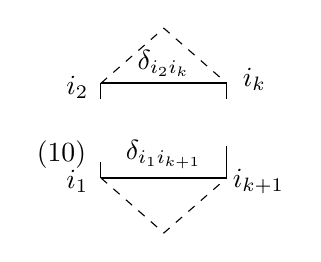
\begin{tikzpicture}[x=1cm,y=1cm]
\node at (-1.3,0) {(10)};
\draw[dashed] (-0.8,0.9)--(0,1.6)--(0.8,0.9); \draw[thick] (-0.8,0.9)--(0.8,0.9);
\draw (-0.8,0.9)--(-0.8,0.7); \draw (0.8,0.9)--(0.8,0.7);
\node at (-1.1,0.85) {$i_2$}; \node at (1.15,0.95) {$i_k$}; \node at (0,1.15) {$\delta_{i_2i_k}$};
\draw[thick] (-0.8,-0.3)--(0.8,-0.3);
\draw (-0.8,-0.3)--(-0.8,-0.1); \draw (0.8,-0.3)--(0.8,0.1);
\draw[dashed] (-0.8,-0.3)--(0,-1)--(0.8,-0.3);
\node at (-1.1,-0.35) {$i_1$}; \node at (1.2,-0.35) {$i_{k+1}$}; \node at (0,0) {$\delta_{i_1i_{k+1}}$};
\end{tikzpicture}
\end{adjustbox}
}

\end{center}
[Справа от (10) зачёркнуто: $\varphi$ \Unclear{GELFAND-P001351}{cancel-phi}{нечитаемый второй зачёркнутый знак}.]
$\varphi$-мы (4) обеспечивают правильную ориентацию при склейке
(из-за эрмитовости!!)
(По-другому выбрав матрицу, можно получить неориентир. пов.)
\begin{center}
\ReaderDiagramPair{figures/gelfand-0146-d10-gelfand-p001351-original.png}{GELFAND-P001351}{%
\begin{adjustbox}{max width=\linewidth}
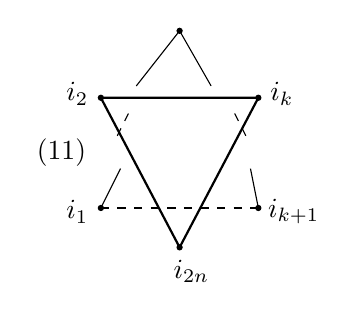
\begin{tikzpicture}[x=1cm,y=1cm]
\node at (-1.5,0) {(11)};
\draw[thick] (-1,0.7)--(1,0.7)--(0,-1.2)--cycle;
\fill (-1,0.7) circle (0.04); \fill (1,0.7) circle (0.04); \fill (0,-1.2) circle (0.04);
\draw (-0.55,0.85)--(0,1.55)--(0.4,0.85); \fill (0,1.55) circle (0.04);
\draw[dashed] (-0.65,0.5)--(-0.8,0.2); \draw[dashed] (0.7,0.5)--(0.85,0.2);
\draw (-0.75,-0.2)--(-1,-0.7); \draw (0.9,-0.2)--(1,-0.7);
\draw[dashed] (-1,-0.7)--(1,-0.7); \fill (-1,-0.7) circle (0.04); \fill (1,-0.7) circle (0.04);
\node at (-1.3,0.75) {$i_2$}; \node at (1.3,0.75) {$i_k$};
\node at (-1.3,-0.75) {$i_1$}; \node at (1.45,-0.75) {$i_{k+1}$}; \node at (0.15,-1.5) {$i_{2n}$};
\end{tikzpicture}
\end{adjustbox}
}

\end{center}
Замкнутые петли $\longrightarrow$ св-во символа Кронекера,
т.е. всегда $N$! Например,
\begin{equation*}
N=\delta_{i_2i_k}\,\delta_{i_ki_{2n}}\,\delta_{i_{2n}i_2}.
\end{equation*}
$\forall$ замкн. цикл даёт $N$!

(12) \underline{Число замкн. циклов = числу вершин в склеив. замкн. фигуре.}

(13) Вклад каждого возможного склеивания (диаграммы)
\begin{equation*}
=N^{-(\#\text{ рёб.})+(\#\text{ вершин})-1}=N^{-2g}.
\end{equation*}
(из-за $\frac N2\operatorname{tr}\varphi^2$ в $\exp$)

\SourcePage{GELFAND-P001352}{86}
Вычислим интеграл (2). Приведём к \Unclear{GELFAND-P001352}{header-word}{диаг.? / сим.? / соб.?} виду:
\begin{equation*}
(14)\quad \varphi_{ij}=\sum_k\Omega^+_{ik}\lambda_k\Omega_{kj},\qquad \Omega\text{ --- унит. матрица}.
\end{equation*}
\begin{equation*}
(15)\quad d^{N^2}\varphi=\left(\prod d\lambda_i\,[\Delta(\lambda)]^2\right)d\Omega,
\end{equation*}
где
\begin{equation*}
\Delta(\lambda)=\prod_{i>j}(\lambda_i-\lambda_j).
\end{equation*}
[Слева зачёркнут номер: \Unclear{GELFAND-P001352}{cancel-number}{$(14)$ / $(16)$}.]
[Справа в рамке: См. Г. \underline{Вейль}: Класс. группы, их инвар. и предст.]
(мера Дайсона).

([Над началом списка: Brezin(?)], Itzykson, Zuber, \underline{Parisi},)
[От Parisi черта вниз:] \underline{метод стох. квантования}

кв. величина $\longmapsto$ марк. процесс.
Среднее вычисляется с пом. уср. по траекториям.
[Слева: работает здесь. Стрелка вниз к (16).]
\begin{equation*}
\begin{aligned}
(16)\quad f_n(N)&\sim\int\prod\left(d\lambda_i\,e^{-N\lambda_i^2/2}\right)\Delta^2(\lambda)
\left(\frac1N\sum_{i=1}^{N}\lambda_i^{2n}\right)=\\
&=\text{\ReaderApparatusRef{1}{1}}
\int\prod\left(d\lambda_i\,e^{-N\lambda_i^2/2}\right)\Delta^2(\lambda)\lambda_1^{2n}\\
&\sim\int\prod\left(d\lambda_i\,e^{-\lambda_i^2/2}\right)\Delta^2(\lambda)\lambda_1^{2n}.
\end{aligned}
\end{equation*}
[От второго равенства черта вниз: симм. по $\lambda_j$.]
(перем. $\lambda_i$ --- выносим \Unclear{GELFAND-P001352}{cancel-rescale}{зачёркнутый одиночный знак} $\sqrt N$ в $\lambda_i$)
\begin{equation*}
(17)\quad \Delta(\lambda)=\det\|(\lambda_\ell)^k\|_{k,\ell}=\det\|H_k(\lambda_\ell)\|.
\end{equation*}
$H_k$ --- любой полином степ. $k$ со старш. коэфф. $1$.
Выберем $H_k$ полиномами Эрмита!!
(с некот. масштабом, чтобы старш. к-тфф. $=1$)
(хорошо, т.к. $H_k$ и $H_\ell$ ортогональны)

Отсюда:
\begin{equation*}
(18)\quad f_n(N)\sim\frac1C\int\prod_{i=1}^{N}\left(d\lambda_i\,e^{-\lambda_i^2/2}\right)\lambda_1^{2n}
\left[\sum_p\prod_{k=1}^{N}H_k(\lambda_{p_k})(-1)^{\operatorname{sgn}(p)}\right]^2=
\end{equation*}
[Под $p$: перестан.]
(Parisi придумали и Bessis приём с полиномами Эрмита)
При возвед. в квадрат: $\forall$ перем. $\lambda_{p_k}$ встреч. ровно $2$ раза.


\ReaderNotesStart{GELFAND-P001352}
\ReaderNote{1}{\Unclear{GELFAND-P001352}{cancel-prefactor}{зачёркнутый одиночный знак перед интегралом}}
\ReaderNotesEnd
\SourcePage{GELFAND-P001353}{unlabelled}
\begin{equation*}
=\sum_{k=0}^{N-1}\frac{\int d\lambda\,e^{-\lambda^2}[H_k(\lambda)]^2\lambda^{2k}}
{\int d\lambda\,e^{-\lambda^2}(H_k(\lambda))^2}.
\end{equation*}
Из справочника (напр. Абрамовица):
\begin{equation*}
(19)\quad \int d\lambda\,e^{i\lambda x}e^{-\lambda^2}[H_k(\lambda)]^2
=\underbrace{\sqrt\pi\,2^n n!}_{\text{сократится со знаменателем}}
e^{-x^2/4}\underbrace{L_n(x^2/2)}_{\text{полин. Лагерра}}.
\end{equation*}
В итоге получим [стрелка к (20)]:
\begin{equation*}
(20)\quad \sum_{n=0}^{\infty}\frac{(-x^2/2)^n}{(2n)!!}f_n(N)
=e^{-x^2/4}\sum_{i=0}^{N-1}L_i(x^2/2)
=e^{-x^2/4}\underbrace{L^1_{N-1}(x^2/2)}_{\text{присоед. полиномы Лагерра}}.
\end{equation*}
Нас здесь \Unclear{GELFAND-P001353}{asympt-word}{наиболее? / интерес.?} асимпт. при $N\to\infty$. Составим произв. ф-ю:
[Зачёркнуто перед (21): $F(x,t)$\Unclear{GELFAND-P001353}{cancel-21}{последний одиночный знак}.]
\begin{equation*}
(21)\quad f_n(t)=\sum_N t^N f_n(N).
\end{equation*}
Для неё ответ:
\begin{equation*}
(22)\quad f_n(t)=\frac{(2n)!}{n!}\frac{(t+1)^n}{(1-t)^{n+2}}.
\end{equation*}
Нас интерес. разлож. в \underline{ряд} по \underline{$t$}.
\underline{Захаревич: ответ (по D. Zagier'у)}
\begin{equation*}
(23)\quad \sum_{g=0}^{\infty}\frac{(n+1)!(n-2g)!}{(2n)!}\,f_g^n x^g
=\left(\frac{\sqrt{x/2}}{\operatorname{th}\sqrt{x/2}}\right)^{n+1}.
\end{equation*}
[На левом поле отдельно: (]
(при $n-2g<0$ надо домножить на $(2n)!$ и перенести в правую часть)
$f_g^n(n-2g)!$ тем самым опред. и при $2g>n$(!).

\underline{Вариант:}
\underline{2 другие комбинат. задачи} (рассматривались Казаковым и Мигдалом).
\tikz{\node[draw,circle,inner sep=1pt] {1};} Как замостить $2n$-уг. $k$ тр-ками, чтобы возникающая поверхность имела род $g$.
[Зачёркнутая строка: Число \Unclear{GELFAND-P001353}{cancel-variant-line}{скл.?}.]
\begin{center}
\ReaderDiagramPair{figures/gelfand-0146-d11-gelfand-p001353-original.png}{GELFAND-P001353}{%
\begin{adjustbox}{max width=\linewidth}
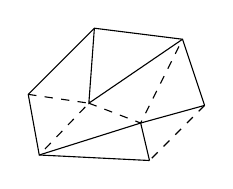
\begin{tikzpicture}[scale=1.4]
\draw (-.60,.10)--(0,.70)--(.80,.60)--(1,0);
\draw (.50,-.50)--(-.50,-.45)--(-.60,.10);
\draw[dashed] (1,0)--(.50,-.50);
\draw (0,.70)--(-.05,.02)--(.80,.60);
\draw (-.50,-.45)--(.42,-.16)--(1,0);
\draw (.42,-.16)--(.50,-.50);
\draw[dashed] (-.60,.10)--(-.05,.02)--(-.50,-.45);
\draw[dashed] (-.05,.02)--(.42,-.16)--(.80,.60);
\end{tikzpicture}
\end{adjustbox}
}

\end{center}
(разреш. пришивать ручки!)
(Симплиц. комплекс заданного рода) $f_k^{2n}(g)$ (Bessis).
(Число Триангуляций \Incomplete{GELFAND-P001353}{cancel-bottom-word}{неразобранное зачёркнутое слово} пов. рода $g$ с $k$-ти треугол., [ниже слева продолжение:] $2n$-угольниками)

\SourcePage{GELFAND-P001354}{87}
(1971--79 г. Itzykson и др.)
\tikz{\node[draw,circle,inner sep=1pt] {2};}
\begin{center}
\ReaderDiagramPair{figures/gelfand-0146-d12-gelfand-p001354-original.png}{GELFAND-P001354}{%
\begin{adjustbox}{max width=\linewidth}
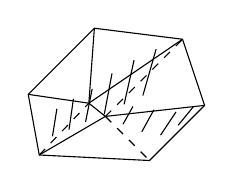
\begin{tikzpicture}[scale=1.4]
\draw (-.60,.10)--(0,.70)--(.80,.60)--(1,0)--(.50,-.50)--(-.50,-.45)--(-.60,.10);
\draw (0,.70)--(-.05,.02)--(.80,.60);
\draw (-.50,-.45)--(.10,-.10)--(1,0);
\draw (-.60,.10)--(-.05,.02)--(.10,-.10);
\draw[dashed] (.10,-.10)--(.50,-.50);
\draw[dashed] (.10,-.10)--(.80,.60);
\draw[dashed] (-.50,-.45)--(-.05,.02);
\draw (-.38,-.28)--(-.34,-.03);
\draw (-.23,-.22)--(-.19,.06);
\draw (-.08,-.15)--(-.02,.15);
\draw (.09,-.08)--(.16,.29);
\draw (.27,.01)--(.36,.41);
\draw (.44,.09)--(.56,.51);
\draw (.26,-.17)--(.35,-.01);
\draw (.43,-.24)--(.54,-.04);
\draw (.60,-.27)--(.74,-.06);
\draw (.76,-.18)--(.90,-.01);
\end{tikzpicture}
\end{adjustbox}
}

\end{center}
То же, но раскрашиваем и фиксир. склейку границы, раскр. бел. и чёрный цвет.

\SourcePage{GELFAND-P001355}{unlabelled}
\underline{9/III--87.} Сем. Гельфанда.
\underline{И. М. Г.} Есть работа, в к-рой сказано следующее; рассм.
\begin{equation*}
z\longmapsto\frac{\alpha z+\beta}{\gamma z+\delta},\qquad
\alpha,\beta,\gamma,\delta\in\mathbb Z,
\end{equation*}
[После $\mathbb Z$ зачёркнуто: \Unclear{GELFAND-P001355}{cancel-after-z}{нечитаемая короткая математическая запись}.]
в полупл., $\operatorname{Im}z>0$; $\alpha\delta-\gamma\beta>0$.
[Зачёркнуто перед Есть: \Unclear{GELFAND-P001355}{cancel-before-exists}{в кр-ве?}.]
Есть мн-ва ненулевой промежут. хаусд. меры,
к-рые возникают в связ. с \underline{осн. серией}.

\underline{Гипотеза}: факторы возникают у предст. $\infty$-мерных групп.
В физике возник. факторы типа $\overline{III}_{\infty}$,
среди них \Unclear{GELFAND-P001355}{physics-ending}{ровно 1 непрерывности?}.

\underline{\Unclear{GELFAND-P001355}{list-heading}{Заболезненности?}}:
а) \Unclear{GELFAND-P001355}{list-first-word}{фракторы? / фракталы?};
б) атракторы; в) хаос; хаусдорфовые меры и \Unclear{GELFAND-P001355}{list-series}{осн. серии? / беск. серии?};
г) характеристические функции.

\underline{Бейлинсон А.}
\underline{Основные факты о $\zeta$-функции Римана и её обобщениях.}
\begin{equation*}
\zeta(s)=\sum_{n=1}^{\infty}\frac1{n^s}.
\end{equation*}
1. Эйлерово произведение:
\begin{equation*}
\zeta(s)=\prod_p(1-p^{-s})^{-1}.
\end{equation*}
2. Аналитическое продолжение: простой полюс при $s=1$, в ост. точках голоморфна.

3. Функциональное уравнение. Введём ещё такую $\zeta$-ф-ю:
\begin{equation*}
\zeta^*(s)=\underbrace{\pi^{-s/2}\Gamma(s/2)}_{\text{Эйлеров множитель с номером }\infty}\zeta(s),
\end{equation*}
тогда $\zeta^*(s)$ инвар. отн. замены $s\to1-s$.
(в отличие от $p$-метрии)

[На левом поле: \underline{Зам. 1.} \underline{Кириллова}.]
\Unclear{GELFAND-P001355}{bottom-prefix}{$\pi$ / $\Pi$}
[Зачёркнуто: \Unclear{GELFAND-P001355}{bottom-cancel}{нечитаемый короткий знак}.]
множитель --- \Unclear{GELFAND-P001355}{bottom-word}{семей? / семья? / слой?} $s$-мерных мер.

\SourcePage{GELFAND-P001356}{unlabelled}
\begin{equation*}
\mathbb R^*\qquad t^{-s}\qquad e^{-t^2}.
\end{equation*}
$\Gamma$ возникает как пр. Меллина.
\begin{equation*}
\mathbb Q_p^*\qquad |t|^s\qquad\underbrace{\text{хар. ф-я }(\mathbb Z_p\setminus0)}_{\text{откр. подгруппа}}\subset\mathbb Q_p^*.
\end{equation*}
её аналог в $\mathbb R^*$ \Unclear{GELFAND-P001356}{analogue-abbrev}{уд. / уб.} гауссовой \underline{exp}.

4. Тривиальные нули: из функц. ур-я ясно, что $\zeta(s)$ имеет нули
(1 кратные) при $s=-2k$, $k\in\mathbb Z$, $k>0$ (из-за $\Gamma$-множителя).
[Ниже короткая зачёркнутая группа: \Unclear{GELFAND-P001356}{cancel-under-four}{нечитаемая короткая зачёркнутая группа}.]

5. Рациональные значения:
\begin{equation*}
\zeta(1-n)=-\frac{B_n}{n}.
\end{equation*}
(в отриц. точках)
[Перед $(t\,d/dt)^n$ зачёркнуто: \Unclear{GELFAND-P001356}{cancel-before-derivative}{нечитаемая короткая зачёркнутая группа}.]
\begin{equation*}
\zeta(-n)=\sum k^n=\left.\left(t\frac d{dt}\right)^n\frac1{1-t}\right|_{t=1}\qquad\star.
\end{equation*}
(точнее, надо взять знач. 1-го регул. члена)

6. Формулы регуляторов: $\forall n$, $\exists$ естеств. подгруппа в $\mathbb R$,
$\Gamma_n\subset\mathbb R$, такая что
[Зачёркнута строка: $\zeta(1-2n)=(\operatorname{vol}\mathbb R/\Gamma_n)\cdot(\text{рац. число})$.]
\begin{equation*}
\zeta'(-2n)=(\operatorname{vol}\mathbb R/\Gamma_n)\cdot(\text{рац. число}).
\end{equation*}
$\Gamma_n$ --- образ $K_{4n+1}(\mathbb Z)$ в $\mathbb R$.

7. Арифметич. св-ва чисел Бернулли: $p$-адич. св-ва $\zeta(1-n)$.
\begin{equation*}
\zeta(s)(1-p^{-s})
\end{equation*}
\begin{equation*}
\zeta(1-n)(1-p^{-1+n})=\int_{\mathbb Z_p^*}x^{1-n}\,d\mu,
\end{equation*}
где $d\mu$ --- естеств. мера на $\mathbb Z_p^*$ (со знач. в $\mathbb Z_p$).
[Слева от следующей строки зачёркнуто: \Unclear{GELFAND-P001356}{cancel-left-units}{знак, похожий на E}.]
\begin{equation*}
\mathbb Z_p^*=(1+p\mathbb Z_p)\times\sqrt[p-1]{1},\qquad ((p-1)\text{-ые корни}).
\end{equation*}
Мн-во характеров \Unclear{GELFAND-P001356}{character-word}{сил?} $\mathbb Z_p^*$ состоит из $(p-1)$ компонент.

8. Гипотеза Римана.

9. Связь с распределением простых чисел.
\SourcePage{GELFAND-P001357}{91}
% Прямой просмотр исходного PNG 2408 x 3448; OCR не применялось.
% Координаты: (left, top, right, bottom), пиксели оригинала, начало (0,0)
% в левом верхнем углу; правый и нижний пределы не включаются.
% Масштабы ниже относятся только к просмотру; новых пикселей источника нет.
% review top-heading: bbox=(205, 25, 1110, 140); nearest-neighbour x3
% review top-definition: bbox=(185, 140, 1150, 430); nearest-neighbour x3
% review euler-product: bbox=(280, 430, 1670, 600); nearest-neighbour x3
% review closure-line: bbox=(175, 585, 2160, 795); nearest-neighbour x2
% review embedding-line: bbox=(185, 755, 1355, 900); nearest-neighbour x3
% review invariance: bbox=(255, 890, 1950, 1010); nearest-neighbour x3
% review inertia-heading: bbox=(235, 1000, 950, 1260); nearest-neighbour x3
% review trivial-action: bbox=(350, 1250, 1230, 1430); nearest-neighbour x3
% review rings-diagram: bbox=(1380, 1030, 2080, 1435); nearest-neighbour x3
% review inertia-diagram: bbox=(175, 1410, 1380, 1830); nearest-neighbour x2
% review frobenius-note: bbox=(1010, 1640, 2075, 1990); nearest-neighbour x3
% review ramification: bbox=(210, 1950, 2000, 2215); nearest-neighbour x3
% review bibliography: bbox=(180, 2210, 1730, 2360); nearest-neighbour x3
% review local-factor: bbox=(235, 2340, 1330, 2500); nearest-neighbour x3
% review example1-heading: bbox=(180, 2480, 1080, 2620); nearest-neighbour x3
% review example1-text: bbox=(195, 2580, 2200, 2750); nearest-neighbour x3
% review galois-character: bbox=(195, 2730, 1310, 3010); nearest-neighbour x3
% review dirichlet-series: bbox=(275, 2990, 1660, 3265); nearest-neighbour x3
% review inertia-margin: bbox=(180, 1605, 455, 1840); nearest-neighbour x6
% review frobenius-leader: bbox=(995, 1680, 1195, 1850); nearest-neighbour x7
% review cancellations-top: bbox=(415, 240, 525, 410); nearest-neighbour x8
% review cancellations-closure: bbox=(195, 610, 455, 810); nearest-neighbour x6
% review ramification-word: bbox=(590, 1970, 790, 2065); nearest-neighbour x6
% review ramification-ending: bbox=(1575, 1955, 1930, 2065); nearest-neighbour x5
% review inertia-margin-text: bbox=(195, 1615, 400, 1745); nearest-neighbour x8
% review inertia-root: bbox=(305, 1660, 396, 1773); nearest-neighbour x10
% review bibliography-title: bbox=(1030, 2215, 1730, 2345); nearest-neighbour x4
% review sum-index: bbox=(510, 3120, 741, 3225); nearest-neighbour x7
% review galois-character-verb: bbox=(510, 2738, 1145, 2845); nearest-neighbour x4
% review embedding-arrow: bbox=(928, 780, 1053, 859); nearest-neighbour x9
% review compare-field-word: bbox=(890, 592, 1090, 704); nearest-neighbour x6
% review inertia-margin-final: bbox=(182, 1518, 450, 1845); nearest-neighbour x4
% review page-label: bbox=(2230, 46, 2384, 198); nearest-neighbour x5
% review almost-all-compare: bbox=(785, 1948, 979, 2072); nearest-neighbour x6
% review lower-border: bbox=(0, 3230, 2408, 3448); nearest-neighbour x1

\underline{Обобщения $\zeta$-ф-и Римана.}

$L$-ф-и Артина \quad $L(\rho,s)$

\begin{equation*}
\rho:\operatorname{Gal}\overline{\mathbb{Q}}/\mathbb{Q}
\underset{\text{непрер.}}{\longrightarrow} GL(n,\mathbb{C})
\end{equation*}
[Между $\operatorname{Gal}$ и $\overline{\mathbb{Q}}/\mathbb{Q}$ зачёркнуто:
\Unclear{GELFAND-P001357}{cancellation-galois}{неразборчивые знаки}.]

\begin{equation*}
L(\rho,s)=\prod_p L_p(\rho,s),\qquad p\text{ — простое число}
\end{equation*}

[Зачёркнуто:
\Unclear{GELFAND-P001357}{cancellation-closure-word}{неразборчивое слово}.]
$\overline{\mathbb{Q}}_p$ — алг. замык. поля $\mathbb{Q}_p$, фикс. вложение
$\overline{\mathbb{Q}}\subset\overline{\mathbb{Q}}_p\quad\Rightarrow$

[Под началом строки зачёркнуто:
\Unclear{GELFAND-P001357}{cancellation-closure-formula}{$\mathbb{Q}_p/\mathbb{Q}$ или $\overline{\mathbb{Q}}_p/\mathbb{Q}$}.]

$\Rightarrow$ вложение
$\operatorname{Gal}\overline{\mathbb{Q}}_p/\mathbb{Q}_p
\hookrightarrow\operatorname{Gal}\overline{\mathbb{Q}}/\mathbb{Q}$

инвар. определён только класс сопряженности этих отобр.

Группа инерции:
\begin{equation*}
I\hookrightarrow\operatorname{Gal}\overline{\mathbb{Q}}_p/\mathbb{Q}_p
\end{equation*}
трив. действ. на $\overline{\mathbb{F}}_p=\overline{\mathbb{Z}/p\mathbb{Z}}$

% Правая схема: верхняя правая вершина не соединена видимой стрелкой;
% вертикальных стрелок между рядами в оригинале нет.
\begin{center}
\begin{adjustbox}{max width=\linewidth}
\begin{tikzcd}[column sep=large,row sep=large]
\overline{\mathbb{Z}/p\mathbb{Z}} &
\overline{\mathbb{Z}}_p \arrow[l] &
\overline{\mathbb{Q}}_p \\
\mathbb{Z}/p\mathbb{Z} &
\mathbb{Z}_p \arrow[l] \arrow[r,hook] &
\mathbb{Q}_p
\end{tikzcd}
\end{adjustbox}
\end{center}

\begin{center}
\begin{adjustbox}{max width=\linewidth}
\begin{tikzcd}[column sep=large,row sep=large]
I \arrow[r,hook] &
\operatorname{Gal}\overline{\mathbb{Q}}_p/\mathbb{Q}_p
  \arrow[r,hook] \arrow[d] &
\operatorname{Gal}\overline{\mathbb{Q}}/\mathbb{Q} \\
& \operatorname{Gal}\overline{\mathbb{Z}/p\mathbb{Z}}=\widehat{\mathbb{Z}} &
\end{tikzcd}
\end{adjustbox}
\end{center}

[На левом поле, выноска к $I$:] оставл. на месте $\sqrt[N]{1}$,
$(N,p)=1$

\SourceFigure{GELFAND-P001357}{frobenius-mark}{Под $\widehat{\mathbb{Z}}$, перед словом «образующая», виден короткий вертикальный штрих над наклонной чертой: возможно, подчёркнутое $1$, возможно, выносной знак.}

образующая $\mathrm{Fr}_p$ (элем. Фробениуса $x\mapsto x^p$)

$\rho$ непрер. $\Rightarrow$ для п.в. $p$ кроме кон. числа
$\rho|_I$ тривиально.

Неразветвленные $p$: $\rho(I_p)=1$

\underline{Лит-ра:} \underline{Касселс, Фрелих} “Алг. теория чисел”

\begin{equation*}
L_p(\rho,s)=\det\bigl(1-\rho(\mathrm{Fr}_p)p^{-s}\bigr)^{-1}
\end{equation*}

\underline{Пример 1.} $L$-ф-и Дирихле

$\rho$ — 1-мерные предст. зад. характерами Дирихле
$\chi:(\mathbb{Z}/N\mathbb{Z})^*\longrightarrow\mathbb{C}^*$

По нему строится хар. гр. Галуа
\begin{equation*}
\operatorname{Gal}\overline{\mathbb{Q}}/\mathbb{Q}
\longrightarrow (\mathbb{Z}/N\mathbb{Z})^*
\overset{\chi}{\longrightarrow}\mathbb{C}^*
\end{equation*}

\begin{equation*}
L(\chi,s)=\sum_{(n,N)=1}\frac{\chi(n)}{n^s}
=\prod_{(p,N)=1}\bigl(1-\chi(p)p^{-s}\bigr)^{-1}
\end{equation*}

\SourcePage{GELFAND-P001358}{unlabelled}
% Прямой просмотр исходного PNG 2408 x 3448; OCR не применялось.
% Координаты: (left, top, right, bottom), пиксели оригинала, начало (0,0)
% в левом верхнем углу; правый и нижний пределы не включаются.
% Масштабы ниже относятся только к просмотру; новых пикселей источника нет.
% review example2-heading: bbox=(230, 20, 1140, 285); nearest-neighbour x3
% review induced-text: bbox=(265, 280, 2200, 425); nearest-neighbour x3
% review induced-formula-left: bbox=(445, 405, 1265, 580); nearest-neighbour x3
% review dedekind-formula-right: bbox=(1200, 420, 2275, 730); nearest-neighbour x3
% review properties-top: bbox=(130, 650, 1410, 990); nearest-neighbour x3
% review product-property: bbox=(150, 980, 1210, 1140); nearest-neighbour x3
% review continuation: bbox=(270, 1140, 1220, 1340); nearest-neighbour x3
% review hypothesis: bbox=(220, 1335, 2150, 1605); nearest-neighbour x3
% review functional-equation: bbox=(190, 1625, 1525, 1880); nearest-neighbour x3
% review equation-note: bbox=(170, 1850, 1710, 2160); nearest-neighbour x3
% review continuation-first-words: bbox=(470, 1150, 1185, 1248); nearest-neighbour x4
% review hypothesis-parenthesis: bbox=(730, 1435, 1940, 1535); nearest-neighbour x3
% review epsilon-note-text: bbox=(790, 1890, 1695, 2000); nearest-neighbour x4
% review epsilon-arguments: bbox=(805, 1758, 1050, 1880); nearest-neighbour x8
% review final-line: bbox=(180, 2030, 760, 2150); nearest-neighbour x5
% review continuation-word: bbox=(493, 1147, 663, 1228); nearest-neighbour x8
% review parenthesis-word: bbox=(875, 1440, 1060, 1516); nearest-neighbour x8
% review page-label-area: bbox=(2130, 0, 2408, 340); nearest-neighbour x3
% review hypothesis-adjectives: bbox=(565, 1344, 1170, 1468); nearest-neighbour x4
% review parenthesis-context: bbox=(715, 1400, 1235, 1570); nearest-neighbour x4
% review parenthesis-whole-word: bbox=(910, 1440, 1135, 1538); nearest-neighbour x6
% review lower-frame: bbox=(0, 2110, 2408, 3448); nearest-neighbour x1

\underline{Пример 2.} \quad $K/\mathbb{Q}\subset\overline{\mathbb{Q}}$

[На правом верхнем поле:]
\Unclear{GELFAND-P001358}{upper-right-mark}{одиночный вертикальный штрих; $1$?}

\begin{equation*}
\operatorname{Gal}\overline{\mathbb{Q}}/K
\subset\operatorname{Gal}\overline{\mathbb{Q}}/\mathbb{Q}
\end{equation*}

Берём индуцир. представление и тогда соотв. $L$-ф-я — это $\zeta_K(s)$

\begin{equation*}
\begin{aligned}
L(\operatorname{Ind}_{K/\mathbb{Q}},s)
&=\zeta_K(s)
=\prod_{\substack{p\text{ — простые}\\\text{идеалы в }K}}
\bigl(1-N(p)^{-s}\bigr)^{-1}\\
&=\sum_{\substack{\text{целые}\\\text{идеалы }I\\\text{в }K}}N(I)^{-s}
\end{aligned}
\end{equation*}

\underline{Св-ва}

0. $L(\rho,s)$ однозначно определяет $\rho$

! $K$ \underline{\underline{не}} восстанавливается по $\zeta_K(s)$

\begin{equation*}
L(\rho_1\oplus\rho_2,s)=L(\rho_1,s)L(\rho_2,s)
\end{equation*}

1. \underline{Аналитич. продолжение}

$L$-ф-и \Unclear{GELFAND-P001358}{analytic-word}{поля / п.в.}
голом. продолжаются.

Все мероморфно продолжаются

\underline{Гипотеза.} $\forall$ неприв. нетрив. $\rho$:
$L(\rho,s)$ голоморфно по $s$.

[Вставка под строкой:]
(если \Unclear{GELFAND-P001358}{parenthetical-mark}{$\rho$ / отдельный дугообразный штрих}
\Unclear{GELFAND-P001358}{parenthetical-verb}{пропущ. / неразборчивое сокращение}
через $GL(n,\mathbb{C})$ — ф-я Артина)

Для $l$-адич. представлений сама мероморфность неизвестна

2. Функц. ур-е. Изв. для $L$-ф-й Артина

\begin{equation*}
L^*(\rho,s)=\varepsilon(\rho s)L^*(\rho^*,1-s)
\end{equation*}
[Запись множителя:
\Unclear{GELFAND-P001358}{epsilon-separator}{$\varepsilon(\rho s)$ / $\varepsilon(\rho,s)$}.]

[Под множителем $\varepsilon(\rho s)$ проведена нижняя квадратная скобка; подпись:]
важная $\mathrm{const}$ содержится здесь
(Гаусс. суммы)

Трив. нули и т. д.

\end{document}
